\documentclass[a4paper,11pt]{article}
\usepackage{algpseudocode}
\usepackage{amsmath}
\usepackage{amssymb}
\usepackage{arydshln}
\usepackage{cite}
\usepackage{color, colortbl}
\usepackage{csvsimple}
\usepackage{float}
\usepackage{graphicx}
\usepackage{indentfirst}
\usepackage{listings}
\usepackage{longtable}
\usepackage[margin=2cm]{geometry}
\usepackage{mathtools}
\usepackage{pdfpages}
\usepackage{pdflscape}
\usepackage{url}
\usepackage{verbatim}

\usepackage{tikz}
\usetikzlibrary{matrix,chains,positioning,decorations.pathreplacing,arrows,calc}

\usepackage[labelformat=simple]{subcaption}% http://ctan.org/pkg/subcaption
\renewcommand\thesubfigure{(\alph{subfigure})}% Allow sub-figure reference to be correctly printed

% \bibliography{mybib}

\definecolor{Green}{rgb}{0.6,1,0.6}
\definecolor{Amber}{rgb}{1,1,0.4}
\definecolor{Red}{rgb}{1,0.6,0.6}

\def\changemargin#1#2{\list{}{\rightmargin#2\leftmargin#1}\item[]}
\let\endchangemargin=\endlist 

\setlength\parindent{24pt}

\usepackage{fancyhdr}
\pagestyle{fancyplain}
\fancyhf{}
\lhead{\fancyplain{}{M.Sc.\ Individual Project Report}}
\rhead{\fancyplain{}{\today}}
\cfoot{\fancyplain{}{\thepage}}

\title{Classification of Pipe Weld Images with Deep Neural Networks\\\Large{--- Final Report ---}}
\author{Dalyac Alexandre\\
       ad6813@ic.ac.uk\\ \\
       \small{Supervisors: Professor Murray Shanahan and Mr Jack Kelly}\\
       \small{Course: CO541, Imperial College London}
}

\begin{document}

\maketitle

\begin{abstract}

{
Automatic image classification experienced a breakthrough in 2012 with the advent of GPU implementations of deep convolutional neural networks (CNNs). These models distinguish themselves by learning features, convolving them to achieve feature equivariance, making use of max pooling operations to achieve robustness to cluttered backgrounds, and a hierarchical structure to enable the learning of complex features with high generalisation performance. This has motivated ControlPoint LLP, a gas \& water infrastructure monitoring company, to explore whether deep learning could be used to automate one of its business services: inspecting photos of polyethylene pipe weld installations to ascertain weld quality. The company reports having previously explored automation with existing businesses, but that the semantic complexity of the visual characteristics to recognise made the task technologically infeasible. \\

After framing the task, this report provides an overview of supervised deep learning, followed by an in-depth explanation of the workings of a deep convolutional neural network, which despite its performance, gathers criticism for its tendency to be used as a black box. The rest of the report goes over the research that was carried out. The first two are mathematical analyses, one of which proposes an explanation for the recent success of the Rectified Linear Unit as the chief activation function of CNNs, the other an explanation for the success of early stopping as a regularisation technique\footnote{Both came about as the result of seeking to understand, with limited assistance, aspects of training deep neural networks; it is uncertain whether existing research exceeds them.}. The next sections are applied and specific to the main task: understanding why learning failed during the first attempts; finding the optimal way to use transfer learning, exploring ways of tackling class imbalance -- including a novel cost function justified by statistical theory which delivered up to 9 additional percentage points in performance; moving away from the common `AlexNet' CNN architecture to conserve spatial information; and final performance results across all tasks.
}
\end{abstract}

\clearpage
\tableofcontents

\clearpage

\section{Acknowledgements}

Many thanks to Prof Murray Shanahan for having been the chief supervisor of this research project; it would not have been possible to pursue it otherwise. 

Thanks to Jack Kelly, the second supervisor of this project, for having created it. Were it not for Jack Kelly, ControlPoint would not have heard of deep learning as a potential technological solution, and I would not have been able to carry out exciting, meaningful research for a real world problem. Jack Kelly shaped not just the research project but a significant portion of my year at Imperial College, by providing guidance towards teaching material on deep learning, encouragement to pursue it, and a group project to apply it. I owe him the discovery of a new passion.

Thanks to Razvan Ranca for precious strategic advice on which experiments to choose for the exploration of hypotheses, help with C++, feedback on the report, as well as musical and caffeine tricks for staying up all night. I look excitingly forward to the times ahead cofounding a machine learning startup together.

Thanks to Alexandre de Brebisson for his great insights into convnet architecture that helped me make sense of experimental results, and the great conversations we had sharing our passion for deep learning.

The Google+ Deep Learning community was perhaps the 2nd most precious resource for this project, after arXiv and before stackoverflow. It provided a large and steady stream of useful resources, comments and guidance. It also seemed like a revolutionary way to be in touch with the world's leading researchers such as Prof Yann LeCun and Prof Yoshua Bengio. I owe particular thanks to Dr Soumith Chintala for his comments on transfer learning and Prof Francisco Zamora-Martinez for his on class imbalance.

\clearpage
\section{Introduction}

\subsection{Explaining the Problem}

The problem consists in building a classifier of pipe weld images capable of detecting the presence of multiple characteristics in each image. Practically speaking, the reason for why this task involves multiple tags per image is because the quality of a pipe weld is assessed not on one, but 17 characteristics, as shown below.

\begin{table}[h]
   \centering
    \begin{tabular}{|l|c|}
    \hline
    Characteristic                 & Penalty Value  \\ \hline
    No Ground Sheet  & ~  5 \\
    No Insertion Depth Markings  & ~ 5 \\
    No Visible Hatch Markings  & ~ 5 \\
    Other  & ~  5 \\
    Photo Does Not Show Enough Of Clamps  & ~ 5 \\
    Photo Does Not Show Enough Of Scrape Zones  & ~ 5 \\
    Fitting Proximity  & ~  15 \\
    Soil Contamination Low Risk  & ~ 15 \\
    Unsuitable Scraping Or Peeling  & ~ 15 \\
    Water Contamination Low Risk  & ~ 15 \\
    Joint Misaligned  & ~  35 \\
    Inadequate Or Incorrect Clamping  & ~ 50 \\
    No Clamp Used  & ~  50 \\
    No Visible Evidence Of Scraping Or Peeling  & ~ 50 \\
    Soil Contamination High Risk  & ~ 50 \\
    Water Contamination High Risk  & ~ 50 \\
    Unsuitable Photo  & ~ 100 \\
    \hline
    \end{tabular}
    \caption {Code Coverage for Request Server}
\end{table} 

At this point, it may help to explain the procedure through which these welds are made, and how pictures of them are taken. The situation is that of fitting two disjoint polyethylene pipes with electrofusion joints \cite{control-point}, in the context of gas or water infrastructure. Since the jointing is done by hand, in an industry affected with alleged `poor quality workmanship', and is most often followed by burial of the pipe under the ground, poor joints occur with relative frequency \cite{control-point}. Since a contamination can cost up to £100,000 \cite{control-point}, there exists a strong case for putting in place protocols to reduce the likelihood of such an event. ControlPoint currently has one in place in which, following the welding of a joint, the on-site worker sends one or more photos, at arm's length, of the completed joint. \\

\begin{figure}[h!]       
    \fbox{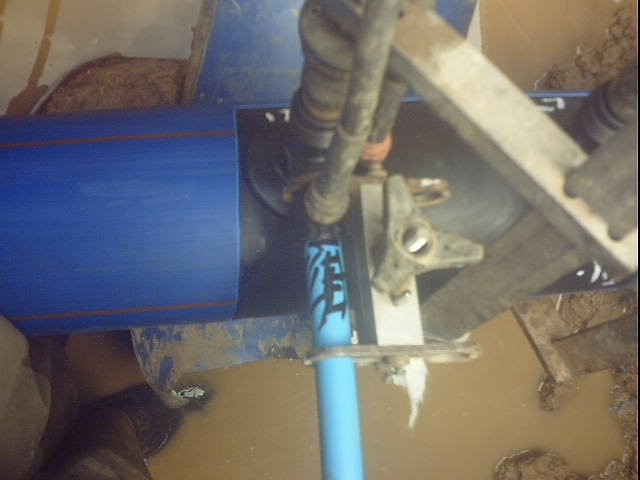
\includegraphics[scale=0.22]{images/soilcontam2.jpg}}   
    \hspace{5px}
    \fbox{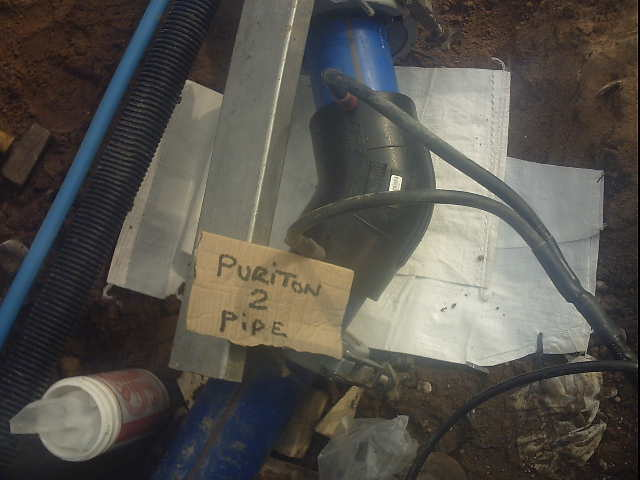
\includegraphics[scale=0.22]{images/watercontam1.jpg}}
    \hspace{5px}
    \fbox{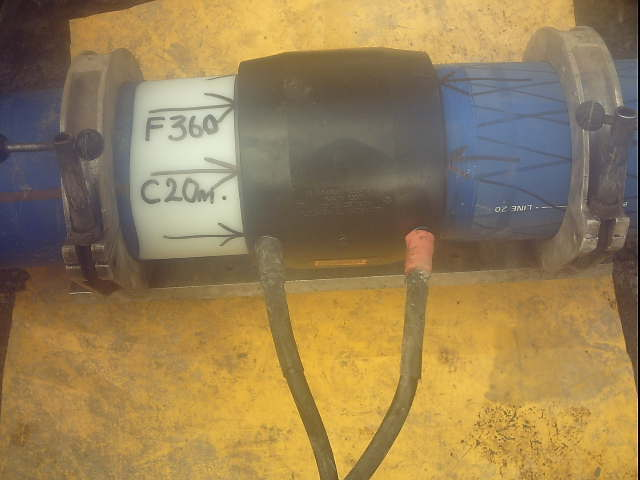
\includegraphics[scale=0.22]{images/perfect2.jpg}}
    \caption{soil contamination risk, water contamination risk, no risk}
    \label{materialflowChart}
\end{figure}


These images are then manually inspected at the ControlPoint headquarters and checked for the presence of the adverse characteristics listed above. The joint is accepted and counted as finished if the number of penalty points is sufficiently low (the threshold varies from an installation contractor to the next, but 50 and above is generally considered as unacceptable). Although these characteristics are all outer observations of the pipe fitting, they have shown to be very good indicators of the quality of the weld \cite{control-point}. Manual inspection of the pipes is not only expensive, but also delaying: as images are queued for inspection, so is the completion of a pipe fitting. Contractors are often under tight operational time constraints in order to keep the shutting off of gas or water access to a minimum, so the protocol can be a significant impediment. Automated, immediate classification would therefore bring strong benefits.

\subsection{Formalising the problem: Multi-Instance Multi-Label Supervised Learning}

The problem of learning to classify pipe weld images from a labelled dataset is a Multi-Instance Multi-Label (MIML) supervised learning classification problem \cite{MIML}: \\

%\begin{changemargin}{1cm}{1cm}  
\indent Given an instance space $\mathcal{X}$, a set of class labels $\mathcal{Y}$, a dataset $\{(X_{1},Y_{1}),(X_{2},Y_{2}), ..., (X_{n},Y_{n})\}$,\\ 
\indent learn a function $f : 2^{\mathcal{X}} \rightarrow 2^{\mathcal{Y}}$ where\\  
\indent \indent $X_{i} \subseteq \mathcal{X}$ is a set of instances $\{x_{1}^{(i)}, x_{2}^{(i)}, ..., x_{p_{i}}^{(i)}\}$\\   
\indent \indent $Y_{	i} \subseteq \mathcal{Y}$ is the set of classes $\{y_{1}^{(i)}, y_{2}^{(i)}, ..., y_{p_{i}}^{(i)}\}$ such that $x_{j}^{(i)}$ is an instance of class $y_{j}^{(i)}$ 
\indent \indent $p_{i}$ is the number of class instances (i.e.\ labels) present in $X_{i}$.\\
%\end{changemargin}


This differs from the traditional supervised learning classification task, formally given by: \\ 

\indent Given an instance space $\mathcal{X}$, a set of class labels $\mathcal{Y}$, a dataset $\{(x_{1},y_{1}),(x_{2},y_{2}), ..., (x_{n},y_{n})\}$,\\ 
\indent learn a function $f : \mathcal{X} \rightarrow \mathcal{Y}$ where\\  
\indent \indent $x_{i} \in \mathcal{X}$ is an instance \\   
\indent \indent $y_{	i} \in \mathcal{Y}$ is the class of which $x_{i}$ is an instance.\\

In the case of MIML, not only are there multiple instances present in each case, but the number of instances is unknown. MIML has been used in the image classification literature when one wishes to identify all objects which are present in the image \cite{MIML}. Although in this case, the motivation is to look out for a specific set of pipe weld visual characteristics, the problem is actually conceptually the same; the number of identifiable classes is simply lower. \\


\subsection{Challenges specific to the Pipe Weld Classification Task}

A number of significant challenges have arisen from this task: multi-tagging, domain change, small dataset size (by deep learning standards) and class imbalance. Before going into them, an overview of the data is given below. \\

\subsubsection{Data Overview}
% \subsubsection{Visual Inspection}
% \subsubsection{Analysis}
% \paragraph{ANOVA}
% \paragraph{t-SNE}


ControlPoint recently upgraded the photographical equipment with which photos are taken (from 'Redbox' equipment to 'Bluebox' equipment), which means that the resolution and finishing of the photos has been altered. There are 113,865 640x480 'RedBox' images. There are 13,790 1280x960 'BlueBox' images. Label frequencies for the Redbox images are given below.

\begin{table}[h!]
   \centering
    \begin{tabular}{|l|c|c|}
    \hline
    Characteristic                              & ~ Redbox Count  & ~ Bluebox Count \\ \hline
    Fitting Proximity                           & ~  1,233        & ~ 32      \\
    Inadequate Or Incorrect Clamping            & ~ 1,401         & ~ 83      \\
    Joint Misaligned                            & ~ 391           & ~ 35      \\
    No Clamp Used                               & ~ 8,041         & ~ 1,571   \\
    No Ground Sheet                             & ~  30,015       & ~ 5,541   \\
    No Insertion Depth Markings                 & ~ 17,667        & ~ 897     \\
    No Visible Evidence Of Scraping Or Peeling  & ~ 25,499        & ~ 1,410   \\
    No Visible Hatch Markings                   & ~ 28,155        & ~ 3,793   \\
    Other                                       & ~  251          & ~ 103     \\
    Photo Does Not Show Enough Of Clamps        & ~ 5,059         & ~ 363     \\
    Photo Does Not Show Enough Of Scrape Zones  & ~ 21,272        & ~ 2,545   \\
    Soil Contamination High Risk                & ~ 6,541         & ~ 3       \\
    Soil Contamination Low Risk                 & ~ 10            & ~ N/A     \\
    Soil Contamination Risk                     & ~ ?             & ~ 529     \\
    Unsuitable Photo                            & ~ 2             & ~ N/A     \\
    Unsuitable Scraping Or Peeling              & ~ 2,125         & ~ 292     \\
    Water Contamination High Risk               & ~ 1,927         & ~ 9       \\
    Water Contamination Low Risk                & ~ 3             & ~ 7       \\
	Water Contamination Risk                    & ~ ?             & ~ 296     \\
     \hline
    Perfect (no labels)                         & ~ 49,039        & ~ 4,182   \\
    \hline
    \end{tabular}
    \caption {Count of Redbox images with given label}
\end{table} 


\subsubsection{Semantic Complexity}

Certain visual characteristics are semantically more complex than normal object classes, because ControlPoint has rules for what counts to raise a flag depending on the nature of the joint. For example, in the case of clamp detection, for tapping-T joints, for the Redbox images, the glint of a slim portion of a clamp is sufficient to judge it present. \\

\begin{figure}[h!]
	\centering
	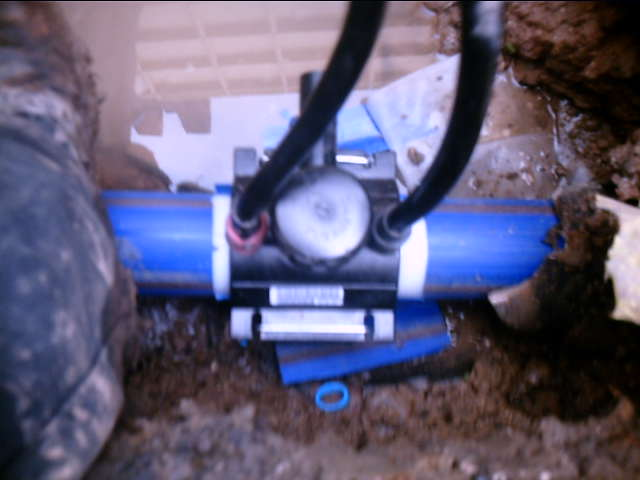
\includegraphics[width=0.35\linewidth]{images/tapping-T.jpg}
	\caption{The clamp wraps around under the pipe - the glint of a metal rod gives it away}
\end{figure}

Worse still, sometimes the presence of clamps `does not count': these are cases for which the purpose of the clamp is other than to secure the welding. Therefore, if such a clamp is present, but the clamp that serves to secure the weld is absent, then the image is assigned the `No Clamps' label. For example, bottom left, a clamp can clearly be seen, but it's not a weld clamp. So this image should have a `No Clamps' flag raised (sadly, it doesn't). Bottom right: the thin metallic clamp that is fastened on the vertical pipe is not the clamp we're interested in. The glint from the thin metallic rod going along the thick, horizontal pipe tells us that a tapping-T clamp is present, even though that clamp is hidden underneath the pipe. 

\begin{figure}
    \centering
    \begin{minipage}[b]{\textwidth}
      \begin{subfigure}{.5\textwidth} 
        \centering
        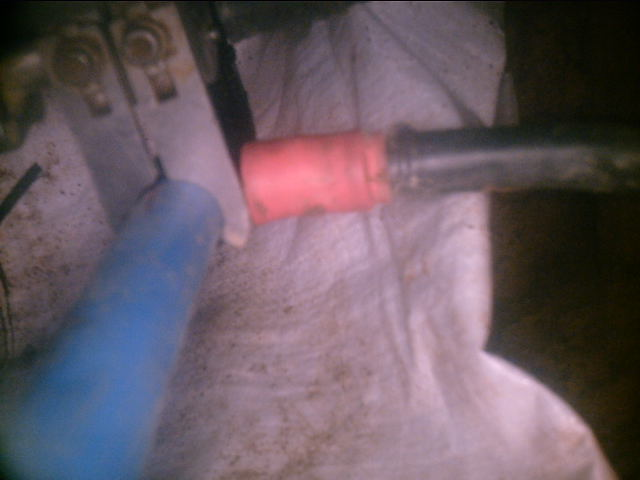
\includegraphics[scale=0.3]{images/truly_confusing_1.jpg}
        % Add \par\vspace*{20pt} here and...
        \caption{The clamp is not a weld clamp}\label{fig:2a}
      \end{subfigure}%
      \begin{subfigure}{.5\textwidth} 
        \centering
        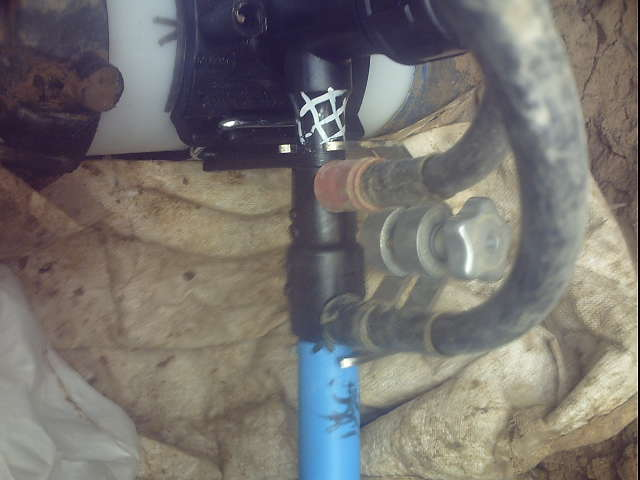
\includegraphics[scale=0.3]{images/truly_confusing_2.jpg}
        % ...here to lower the subcaptions and...
        \caption{The clamp on the vertical rod is not a weld clamp}\label{fig:2b}
      \end{subfigure} \par \vspace*{20pt} % ...remove them from here
    \end{minipage}%
\end{figure}


\subsubsection{Domain Change}

%This makes learning very difficult, as a class can be pictured as a disjoint set of subclasses, some of which fine-grained, and that one subclass could trigger a false positive of another class.\\

Domain change can be lethal to computer vision algorithms: for example, a feature learned (at the pixel level) from the 640x480 Redbox images could end up being out of scale for the 1280x960 Bluebox images. However, this simple example is not relevant to a CNN implementation, since the largest networks can only manage 256x256 images, so Bluebox and Redbox images will both be downsized to identical resolutions. However, of greater concern is the difference in image sharpness between Redbox and Bluebox images, as can be seen below. It remains to be seen how a CNN could be made to deal with this type of domain change.

\begin{figure}
    \centering
    \begin{minipage}[b]{\textwidth}
      \begin{subfigure}{.5\textwidth} 
        \centering
        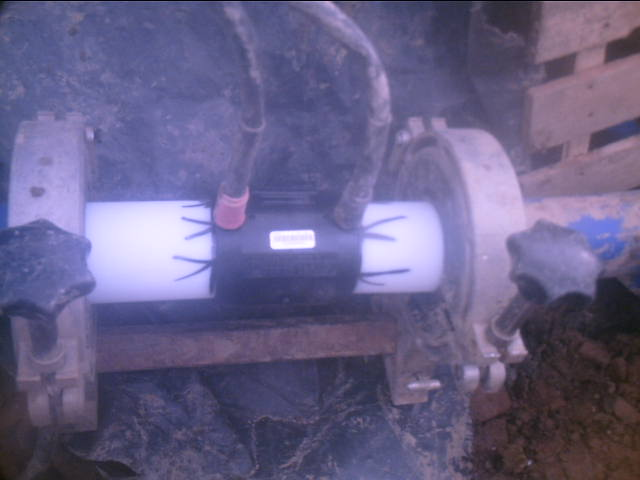
\includegraphics[scale=0.34]{images/perfect3.jpg}
        % Add \par\vspace*{20pt} here and...
        \caption{A Redbox photo}\label{fig:2a}
      \end{subfigure}%
      \begin{subfigure}{.5\textwidth} 
        \centering
        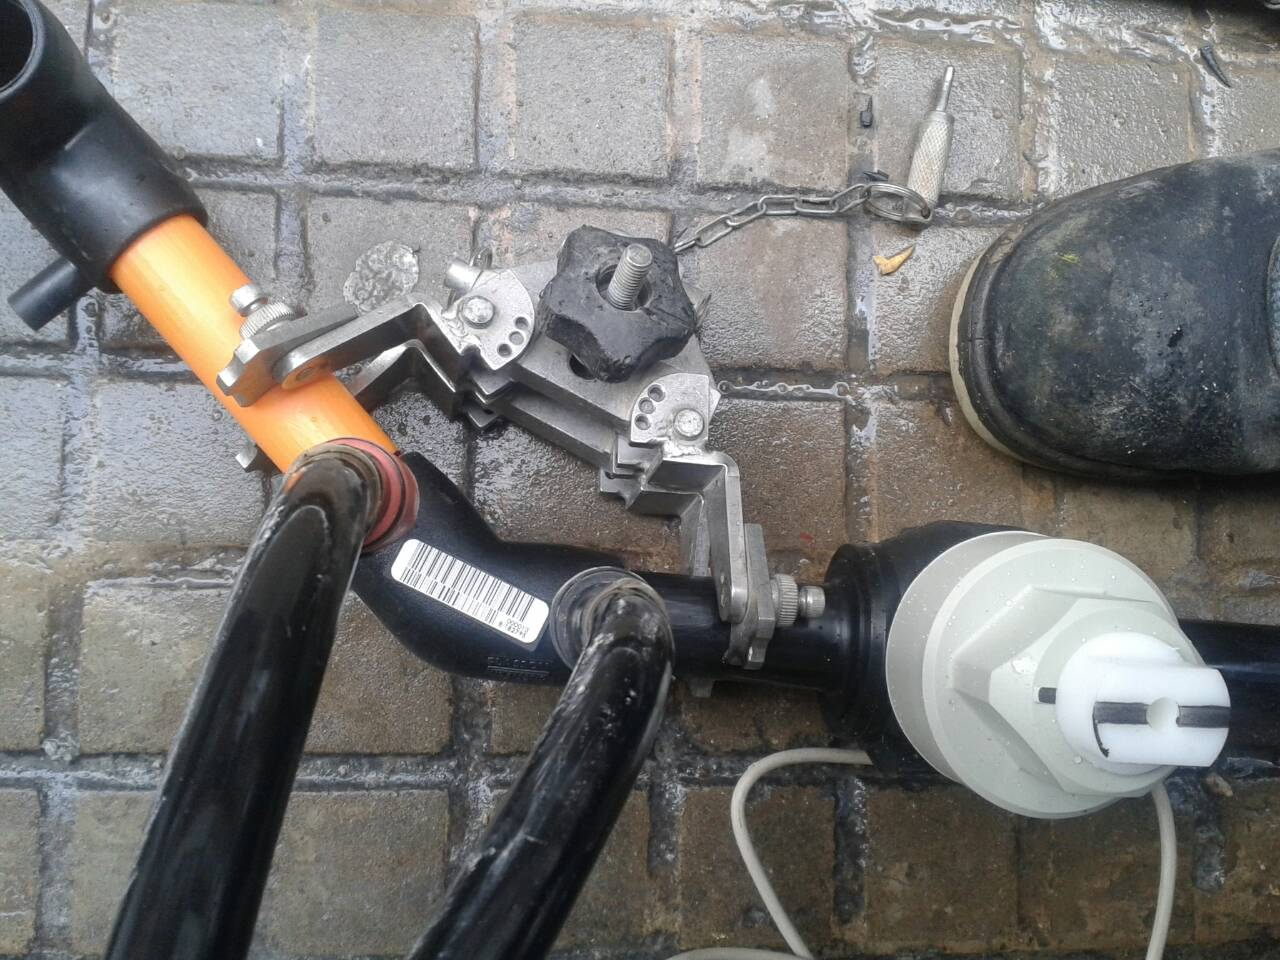
\includegraphics[scale=0.17]{images/niceBluebox_100974.jpg}
        % ...here to lower the subcaptions and...
        \caption{A Bluebox photo}\label{fig:2b}
      \end{subfigure} \par \vspace*{20pt} % ...remove them from here
    \end{minipage}%
\end{figure}

Nevertheless, evidence has been found to suggest that deep neural networks are robust to it: an experiment run by Donahue et al on the \textit{Office} dataset \cite{office}, consisting of images of the same products taken with three different types of photographical equipment (professional studio equipment, digital SLR, webcam) found that their implementation of a deep convolutional neural network produced similar feature representations of two images of the same object even when the two images were taken with different equipment, but that this was not the case when using SURF, the currently best performing set of hand-coded features on the \textit{Office} dataset \cite{surf}. \\


\subsubsection{Small Dataset Size}

Alex Krizhevsky's record-breaking CNN was trained on 1 million images \cite{krizhevsky}. Such a large dataset enabled the training of a 60-million parameter neural network, without leading to overfit. In this case, there are 'only' 5,000, and 43\% of them are images of `perfect' welds, meaning that these are label-less. Training a similarly sized network leads to overfit, but training a smaller network could prevent the network from learning sufficiently abstract and complex features for the task at hand. A solution to consider is that of transfer learning \cite{transfer-learning}, which consists in importing a net which has been pretrained in a similar task with vast amounts of data, and to use it as a feature extractor. This would bring the major advantage that a large network architecture can be used, but the number of free parameters can be reduced to fit the size of the training set by `freezing' backpropagation on the lower layers of the network. Intuitively, it would make sense to freeze the lower (convolutional) layers and to re-train the higher ones, since low-level features (such as edges and corners) are likely to be similar across any object recognition task, but the way in which these features are combined are specific to the objects to detect.

\subsubsection{Class Imbalance}

The dataset suffers from a similar adverse characteristic to that of medical datasets: pathological observations are significantly less frequent that healthy observations. This can make mini-batch training of the network especially difficult. Consider the simple case of training a neural network to learn the following labels: No Clamp Used, Photo Does Not Show Enough Of Clamps, Clamp Detected (this label is not in the list, but can be constructed as the default label). Only 8\% of the Redbox images contain the first label, and only 5\% contain the second label, so if the partial derivatives of the error are computed over a batch of 128 images (as is the case with the best implementations \cite{krizhevsky},\cite{transfer-learning}, \cite{decaf}), one can only expect a handful of them to contain either of the first two labels. Intuively, one may ask: how could I learn to recognise something if I'm hardly ever shown it?\\



\clearpage

\section{Literature Review}

\subsection{Supervised Learning}

Learning in the case of classification consists in using the dataset $\mathcal{D}$ to find the hypothesis function $f^{h}$ that best approximates the unknown function $f^{*} : 2^{\mathcal{X}} \rightarrow 2^{\mathcal{Y}}$ which would perfectly classify any subset of the instance space $\mathcal{X}$. Supervised learning arises when $f^{*}(x)$ is known for every instance in the dataset, i.e.\ when the dataset is labelled and of the form $\{(x_{1},f^{*}(x_{1})),(x_{2},f^{*}(x_{2})), ..., (x_{n},f^{*}(x_{n}))\}$. This means that $|\mathcal{D}|$ points of $f^{*}$ are known, and can be used to fit $f^{h}$ to them, using an appropriate cost function $\mathcal{C}$. $\mathcal{D}$ is therefore referred to as the \textit{training set}. 

Formally, supervised learning therefore consists in finding

\begin{equation}
\label{learning: optimisation equation}
  f^{h} = \operatornamewithlimits{argmin}\limits_{\mathcal{F}}\operatorname{\mathcal{C}}(\mathcal{D})
\end{equation}
  
where $\mathcal{F}$ is the chosen target function space in which to search for $f^{h}$ . \\

\subsection{Approximation vs Generalisation}

It is important to note that supervised learning does not consist in merely finding the function which best fits the training set - the availability of numerous universal approximating function classes (such as the set of all finite order polynomials) would make this a relatively simple task \cite{univ-approx}. The crux of supervised learning is to find a hypothesis function which fits the training set well \textit{and} would fit well to any subset of the instance space, including unseen data. Approximation and generalisation together make up the two optimisation criteria for supervised learning.\\

\subsection{Models of Neurons}

Learning a hypothesis function $f^{h}$ comes down to searching a target function space for the function which minimises the cost function. A function space is defined by a parametrised function equation, and a parameter space. Choosing a deep convolutional neural network with rectified linear neurons sets the parametrised function equation. By explaining the architecture of such a neural network, this subsection justifies the chosen function equation. As for the parameter space, it is $\mathbb{R^{P}}$ (where P is the number of parameters in the network); its continuity must be noted as this enables the use of gradient descent as the optimisation algorithm (as is discussed later). \\

Before we consider the neural network architecture as a whole, let us start with the building block of a neural network: the neuron (mathematically referred to as the \textit{activation function}). Two types of neuron models are used in current state-of-the-art implementations of deep convolutional neural networks: the rectified linear unit and the softmax unit (note that the terms `neuron' and `unit' are used interchangeably). In order to bring out their specific characteristics, we shall first consider two other compatible neuron models: the binary threshold neuron, which is the most intuitive, and the hyperbolic tangent neuron, which is the most analytically appealing. It may also help to know what is being modelled, so a very brief look at a biological neuron shall first be given.

\paragraph{Multipolar Biological Neuron}

\begin{figure}[h!]
	\centering
	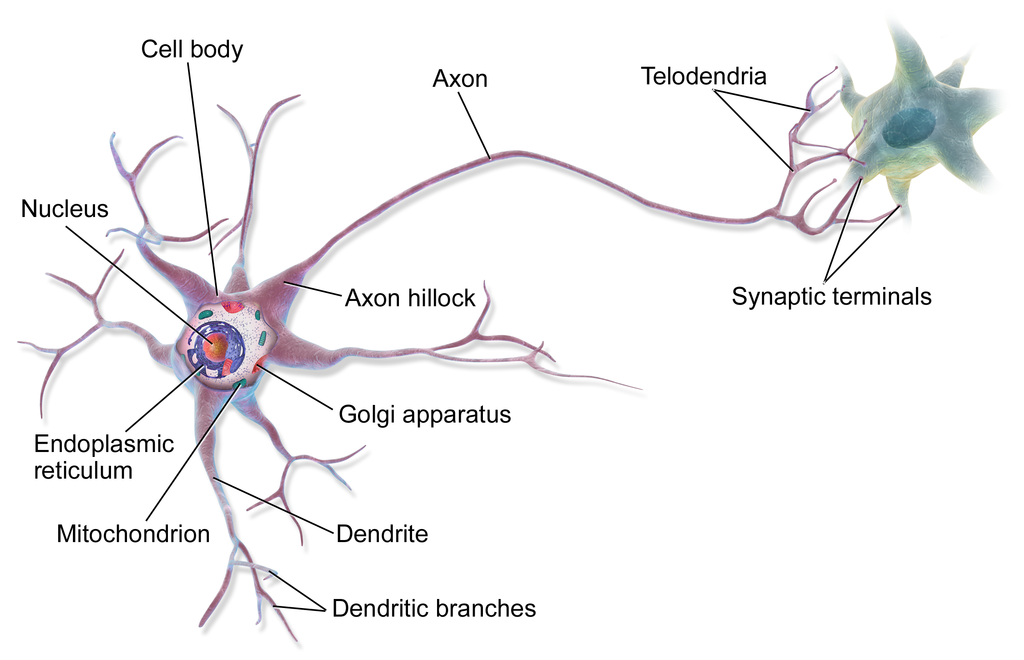
\includegraphics[scale=0.3]{images/Biological_Neuron.png}
	\caption{a multipolar biological neuron}
\end{figure}

A multipolar neuron receives electric charges from neighbouring incoming neurons through its dendritic branches, and sends electric charges to its neighbouring outgoing neurons through its axon. Neurons connect at synapses, which is where the tip of the telodendria of one neuron is in close vicinity of the dendritic branch of another neuron. Because a single axon feeds into all of the telodendria but mutiple dendritic branches feed into the axon hillock, a neuron receives multiple inputs and sends out a single output. Similarly, all of the neuron models below are functions from a multidimensional space to a unidimensional one.\\

\paragraph{Binary Threshold Neuron}
\begin{equation}
y = \begin{cases} 1 & \mbox{if } M <= b + \sum\limits_{i=1}^k x_{i}\cdot w_{i}  \text{ , where } M \text{ is a threshold parameter} \\ 
				  0 & \mbox{otherwise} \end{cases}
\end{equation} \\

Intuitively, $y$ takes a hard decision, just like biological neurons: either a charge is sent, or it isn't. $y$ can be seen as producing spikes, $x_{i}$ as the indicator value of some feature, and $w_[i]$ as a parameter of the function that indicates how important $x_{i}$ is in determining $y$. Although this model is closer than most most to reality, the function is not differentiable, which makes it impossible to use greedy local optimisation learning algorithms - such as gradient descent - which need to compute derivatives involving the activation functions.

\paragraph{Logistic Sigmoid Neuron} 
\begin{equation}
\label{sigmoid neuron}
y = \frac{1}{1 + \exp(-z)} \text{, where } z = \sum\limits_{i=1}^k x_{i}\cdot w_{i}
\end{equation}

Like the binary threshold neuron, the output domain of this neuron is bounded by 0 and 1. But this time, the function is fully differentiable. Moreover, it is nonlinear, which helps to increase performance \cite{DL-book}. To see why, the graph plot below lends itself to the following intuition: if the input x is the amount of evidence for the components of the feature that the neuron detects, and y is the evidence for the feature itself, then the marginal evidence for the feature is decreasing with the amount of evidence for its components (in absolute value terms). 

\begin{figure}[h!]
	\centering
	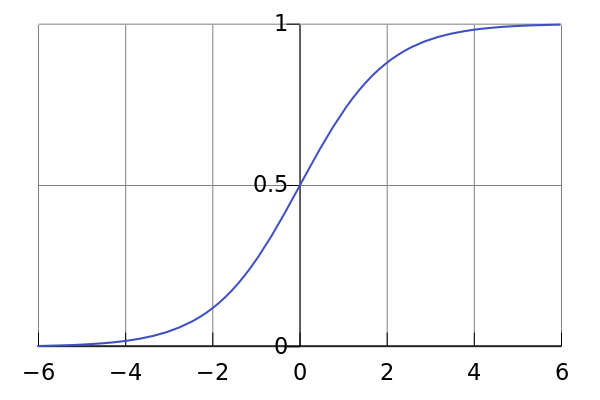
\includegraphics[scale=0.3]{images/sigmoid.png}
	\caption{single-input logistic sigmoid neuron}
\end{figure}

This is like saying that to completely convince y of the total presence or absence of the feature, a lot of evidence is required. However, if there is not much evidence for either case, then y is more lenient. 
A disadvantage of this neuron model is that it is computationally expensive to compute.
                
\paragraph{Rectified Linear Neuron}
\begin{equation}
\label{relu}
y = \max\{0, b + \sum\limits_{i=1}^k x_{i}\cdot w_{i}\}
\end{equation}

As can be seen in the graph plot below, the rectified linear neuron is neither fully differentiable (not at $0$), nor bounded above. Moreover, it only has two slopes, so its derivative with respect to $x_{i}$ can only be one of two values: $0$ or $w_{i}$. Although this may come as a strong downgrade in sophistication compared to the logistic sigmoid neuron, it is so much more efficient to compute (both its value and its partial derivatives) that it enables much larger network implementations\cite{krizhevsky}. Until now, this has more than offset the per-neuron information loss - and saturation risks - of the rectifier versus the sigmoid unit \cite{rectifier}. \\

ReLU introduces a non-linearity with its angular point (a smooth approximation to it is the softplus $f(x) = \log(1 + e^x)$). \\

Explain also the no neighbouring cancellations in pooling. \\

\begin{figure}[h!]
	\centering
	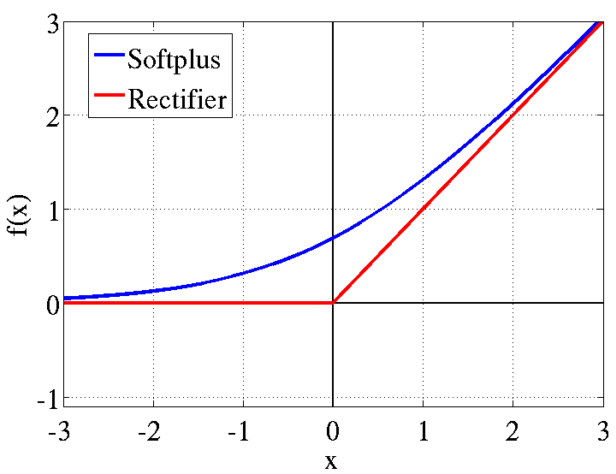
\includegraphics[scale=0.3]{images/rectifier.png}
	\caption{single-input rectified linear neuron}
\end{figure}

\paragraph{Softmax Neuron}
\begin{equation}
\label{}
y_{j} = \frac{\exp(z_{j})}{\sum\limits_{i=1}^k\exp(z_{i})} \text{, where } z_{j} = \sum\limits_{i=1}^k x_{i}\cdot w_{i,j} + b
\end{equation}

The equation of a softmax neuron needs to be understood in the context of a layer of $k$ such neurons within a neural network: therefore, the notation $y_{j}$ corresponds to the output of the $j^{th}$ softmax neuron, and $w_{i,j}$ corresponds to the weight of $x_{i}$ as in input for the $j^{th}$ softmax neuron. A layer of softmax neurons distinguishes itself from others in that neighbouring neurons interact with each other: as can be seen from the equation, the input vectors of all the softmax neurons $z_{1}, z_{2}, ..., z_{k}$ serve to enforce $\sum\limits_{i=1}^k y_{i} = 1$. In other words, the vector $(y_{1}, y_{2}, ..., y_{k})$ defines a probability mass function. This makes the softmax layer ideal for classification: neuron $j$ can be made to represent the probability that the input is an instance of class $j$. Another attractive aspect of the softmax neuron is that its derivative is quick to compute: it is given by $\frac{dy}{dz} = \frac{y}{1-y}$. Note that the name `softmax' comes from the fact that competition between the neurons of a softmax layer results in a sort of smooth indicator function for the max: if a softmax neuron's input is maximal across the inputs of the softmax layer, then the maximum is present there and not anywhere else; the output for that softmax neuron will be close to 1 and the output for the other neurons will be close to zero.\\


\subsection{Feed-forward Architecture}

A feed-forward neural network is a representation of a function in the form of a directed acyclic graph, so this graph can be interpreted both biologically and mathematically. A node represents a neuron as well as an activation function $f$, an edge represents a synapse as well as the composition of two activation functions $f \circ g$, and an edge weight represents the strength of the connection between two neurons as well as a parameter of $f$. The figure below (taken from \cite{DL-book}) illustrates this.

\begin{figure}[h!]
	\centering
	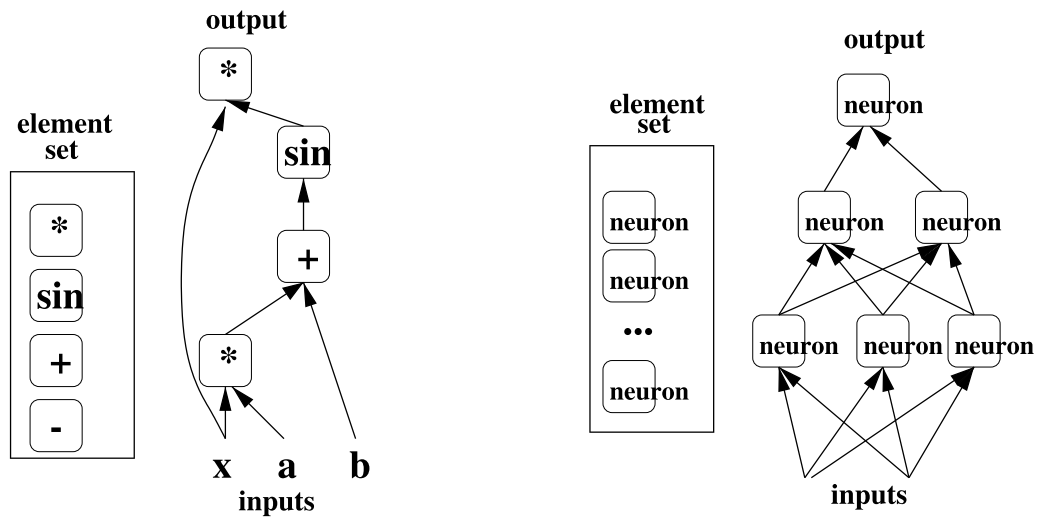
\includegraphics[scale=0.3]{images/NN_math_rep.png}
	\caption{graphical representation of $y = x*sin(a*x+b)$ (source: Bengio 2009)}
\end{figure}

The architecture is feed-forward in the sense that data travels in one direction, from one layer to the other. This defines an input layer (at the bottom) and an output layer (at the top) and enables the representation of a mathematical function.

\paragraph{Shallow Feed-Forward Neural Networks: the Perceptron} 

A feed-forward neural net is called a perceptron if there exist no layers between the input and output layers. The first neural networks, introduced in the 1960s \cite{DL-book}, were of this kind. This architecture severely reduces the function space: for example, with $g_{1}: x \rightarrow sin(s)$, $g_{2}: x,y \rightarrow x*y$, $g_{3}: x,y \rightarrow x+y$ as activation functions (i.e.\ neurons), it cannot represent $f(x) \rightarrow x*sin(a*x+b)$ mentioned above \cite{DL-book}. This was generalised and proved in \textit{Perceptrons: an Introduction to Computation Geometry} by Minsky and Papert (1969) and lead to a move away from artificial neural networks for machine learning by the academic community throughout the 1970s: the so-called `AI Winter' \cite{Russel & Norvig}. 

\paragraph{Deep Feed-Forward Neural Networks: the Multilayer Perceptron} 

The official name for a deep neural network is Multilayer Perceptron (MLP), and can be represented by a directed acyclic graph made up of more than two layers (i.e.\ not just an input and an output layer). These other layers are called hidden layers, because the `roles' of the neurons within them are not set from the start, but learned throughout training. When training is successful, each neuron becomes a feature detector. At this point, it is important to note that feature learning is what sets machine learning with MLPs apart from most other machine learning techniques, in which features are specified by the programmer \cite{DL-book}. It is therefore a strong candidate for classification tasks where features are too numerous, complex or abstract to be hand-coded - which is arguably the case with pipe weld images.\\ 

\begin{figure}[h!]
	\centering
	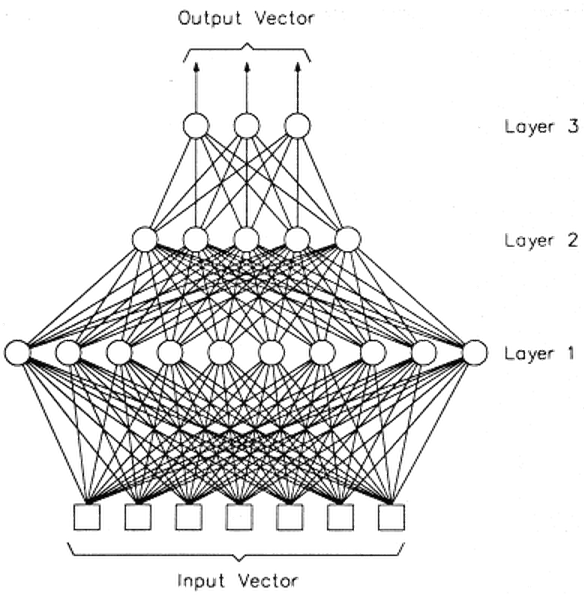
\includegraphics[scale=0.4]{images/MLP.png}
	\caption{Multi Layer Perceptron with 2 hidden layers}
\end{figure}

Mathematically, it was proved in 1989 that MLPs are universal approximators \cite{MLP-univ-approx}; hidden layers therefore increase the size of the function space, and solve the initial limitation faced by perceptrons. \\

Intuitively, having a hidden layer feed into another hidden layer above enables the learning of complex, abstract features, as a higher hidden layer can learn features which combine, build upon and complexify the features detected in the layer below. The neurons of the output layer can be viewed as using information about features in the input to determine the output value. In the case of classification, where each output neuron corresponds to the probability of membership of a specific class, the neuron can be seen as using information about the most abstract features (i.e.\ those closest to defining the entire object) to determine the probability of a class membership. \\

\subsection{Justifying Depth}

To make the case for deep architectures, consider a model with the same number of parameters but fewer layers (i.e.\ a greater number of neurons per layer). (Goodfellow et al 2013) \cite{goodfellow_street_view} ran experiments to compare and found that depth is better: intuitively, if neurons are side by side, they cannot use the computation of their neighbour, whereas with depth, the neurons above can make use of the work done by the neurons below. \\	

\begin{figure}[h!]
	\centering
	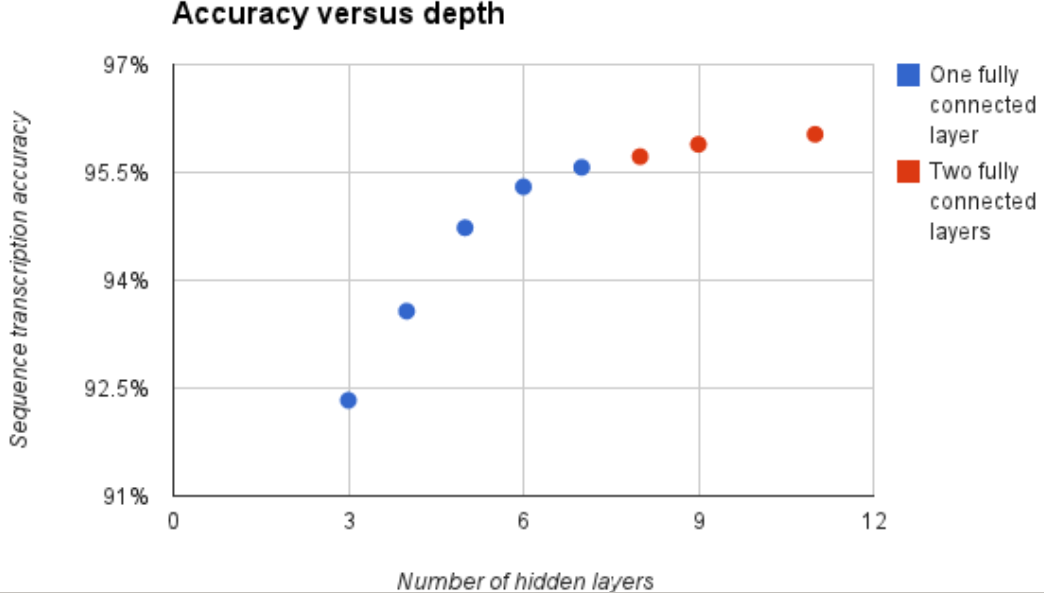
\includegraphics[scale=0.3]{images/more_layers_better.png}
	\caption{LeNet7 architecture: each square is a kernel}
\end{figure}

As a formalisation of the intuition given above, (Bengio 2009) \cite{DL-book} advances that having multiple layers creates a \textbf{distributed representation} of the data, rather than a \textbf{local representation}. Consider for example the one-hot encoding of the integer set $\{0, .., n-1\}$, consisting of n-bit vectors where the i-th bit is 1 if the vector represents the integer i. This encoding is sparse, because every element of the set is represented by a vector of n-1 zeros and one 1. Moreover, it is local, because the k-th vector entry marks the presence of a feature that is present in only a single element, the integer k. On the other hand, the binary representation of the integers ${0, .., n-1}$ is a dense distributed representation, because it requires only $log_2(n)$ bits, and the k-th vector entry marks the presence of a feature that is shared by multiple elements of the set: whether or not not the integer is $\geq 2^k$. The binary representation is richer and more powerful than the one-hot representation because its features are not mutually exclusive: each class (i.e.\ each integer) is represented by a combination of features rather than a unique one. It is in this sense that the representation is distributed, and that the features are general. \\

(Bengio 2009) \cite{DL-book} details the belief that a deep architecture incites such representations, since, by having a neuron feed into multiple neurons of another hidden layer above, the feature it learns will be used by several feature detectors (or eventually, class detectors) above. The crucial benefit of this is generalisation: features learned from data in a specific region of the input space (a.k.a\ data space) are used in other regions of the input space, even if little to no data from this region is present to learn from. It is in this sense that the representation is general, not local. \\

However, it may seem `risky' to be imposing the use of features in regions of the input space that are unknown. `As usual in ML, there is no real free lunch' \cite{Bengio_G+}. Indeed, one can think of this as imposing a prior on the function space to be searched, that is of the form: the observed data can be explained by a number of underlying factors which can be learned without seeing all of their configurations. If the prior is true for the classes we are learning, the gains are large. Successes in deep learning seem to indicate that this prior covers many tasks that humans deal with \cite{Bengio_G+}. This prior is particularly powerful when learning from high dimensional data, where the curse of dimensionality means that a vast majority of the configurations are missing from the training set. \\

\clearpage

\subsection{Backpropagation}

Now that the architecture of a deep neural network has been motivated, the question remains of how to train it. Mathematically: now that the function space has been explained, the question remains of how this space is searched. In the case of feed-forward neural networks and supervised learning, this is done with gradient descent, a local (therefore greedy) optimisation algorithm. Gradient descent relies on the partial derivatives of the error (a.k.a\ cost) function with respect to each parameter of the network; the backpropagation algorithm is an implementation of gradient descent which efficiently computes these values.
  
\subsubsection{Compute Error-Weight Partial Derivatives}

Let $t$ be the target output (with classification, this is the label) and let $y = (y_{1}, y_{2}, ..., y_{P})$ be actual value of the output layer on a training case. (Note that classification is assumed here: there are multiple output neurons, one for each class).

The error is given by 
\begin{equation}
E = \mathcal{C}(t-y)
\end{equation}

where $\mathcal{C}$ is the chosen cost function. The error-weight partial derivatives are given by

\begin{equation}
\frac{\partial{E}}{\partial{w_{ij}}} = \frac{\partial{E}}{\partial{y_{i}}} \cdot \frac{\partial{y_{i}}}{\partial{net}} \cdot \frac{\partial{net}}{\partial{w_{ij}}}
\end{equation}

Since in general, a derivative $\frac{\partial{f}}{\partial{x}}$ is numerically obtained by perturbing $x$ and taking the change in $f(x)$, the advantage with this formula is that instead of individually perturbing each weight $w_{ij}$, only the unit outputs $y_{i}$ are perturbed. In a neural network with $k$ fully connected layers and $n$ units per layer, this amounts to $\Theta(k \cdot n)$ unit perturbations instead of $\Theta(k \cdot n^{2})$ weight perturbations \footnote{the bound on weight perturbations is no longer tight if we drop the assumption of fully connected layers}. Therefore, backpropagation scales linearly with the number of neurons. \\

\subsubsection{Update Weight Values with Gradient Descent}

The learning rule is given by:

\begin{equation}
 w_{i,t+1} = w_{i,t+1} + \tau \cdot \frac{\partial{E}}{\partial{w_{i,t}}}
 \label{eqn:learning_rule}
\end{equation}

Visually, this means that weight values move in the direction that will (locally) reduce the error quickest, i.e.\ the direction of steepest (local) descent on the error surface is taken. Notice that given the learning rule, gradient descent converges (i.e.\ $w_{i,t+1}$ equals $w_{i,t+1}$) when the partial derivative reaches zero. This corresponds to a local minimum on the error surface. In the figure below, two training sessions are illustrated: the only difference is the initialisation of the (two) weights, and the minima attained in each case are not the same. This illustrates a strong shortcoming with backpropagation: parameter values can get stuck in poor local minima.

\begin{figure}[h!]
	\centering
	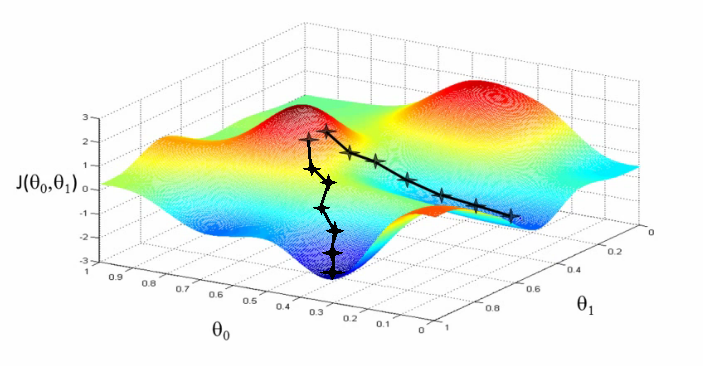
\includegraphics[scale=0.8]{images/local_minima.png}
	\caption{an error surface with poor local minima}
\end{figure}


\subsubsection{Stochastic Gradient Descent}

In practice, in order to ensure use precise weight updates, the partial derivatives are obtained by averaging over a number of training cases (which are often said to be grouped in `mini batches'). This is called Stochastic Gradient Descent \cite{DL-book}, and is also referred to as `mini batch training'.

% \paragraph{cost functions}
% MSE, cross-entropy for softmax

\subsection{Overfit}

As mentioned previously, learning is not a mere approximation problem because the hypothesis function must generalise well to any subset of the instance space. A downside to using highly expressive models such as deep neural networks is the danger of overfit: training may converge to a function that, despite having zero error over the training set (i.e.\ perfectly fits the training set), performs poorly on unseen data. Overfit can be easily understood with the regression example of fitting a polynomial to a set of points sampled uniformly with noise from a curve, as shown below. 

\begin{figure}[h!]
	\centering
	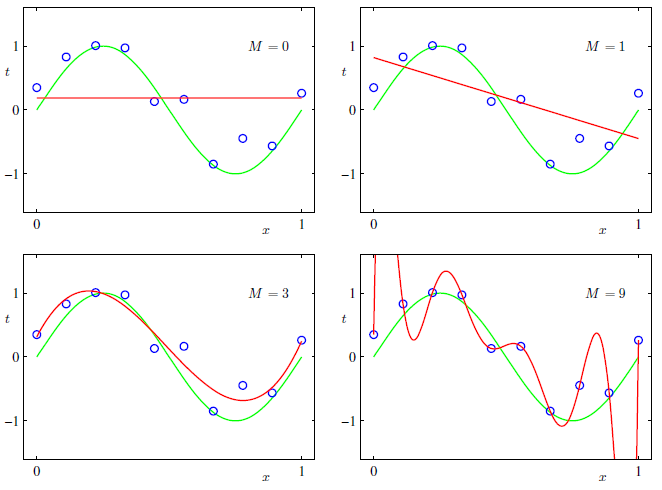
\includegraphics[scale=0.8]{images/overfit.png}
	\caption{Overfit as polynomial order increases (source: Bishop 2010)}
\end{figure}

$M$ is the order of the polynomial used and governs the expressiveness of the model. Clearly, the fit of the model increases with $M$, but one can see that for the case $M = 9$, the given polynomial fits the true (green) function poorly: in other words, the model generalises poorly. How well the model generalises can be evaluated by measuring the fit an another sample of points. \\

\subsubsection{Cross Validation}

This is the intuition behind cross validation, which consists in separating the labelled dataset into a training set, a validation set and a test set. The partial derivatives are computed from the error over the training set, but the function that is retained at the end of training is the one that minimises the error over the validation set, and its performance is measured on the test set. The distinction between the test set and the validation set is to obtain a stochastically impartial measure of performance: since the function is chosen to minimise the error over the validation set, there could be some non-negligible overfit to the validation set which can only be reflected by assessing the function's performance on yet another set. \\

In practice, \textbf{early stopping} is the form of cross validation used: training continues while the validation error decreases, and terminates as soon as it begins to rise (even if the training error is still decreasing). One may realise that a non negligible assumption underlies this: convexity of the time series of the validation error, i.e.\ once the validation error has reached a minimum, then this is the global minimum. This property is always observed in practice \cite{ML-book}, but one may wonder why. Section `Analyis 2' of the report proposes a mathematical explanation of this. \\

\subsubsection{Data Augmentation}

Consider the polynomial overfit figure above: the points on the fitted curve which are furthest away from the true curve are those which lie far away (in terms of X axis distance) from the sampled points. If the sample contained points with those X coordinates, the fitted polynomial would not have scored as low an error, and would not have been the polynomial of best fit. In other words, more data would have reduced overfit. This is what underlies artificial data augmentation, introduced by (Ciresan et al 2011) \cite{data-aug}, which consists in applying label preserving transformations to the training set, i.e.\ `affine (translation, rotation, scaling, horizontal shearing) and elastic deformations'. This was reported to bring the test error rate on MNIST (a benchmark dataset for image classification consisting of 100,000 28x28 greyscale images of handwritten digits, where each digit defines a class) down from 0.40\% to 0.27\%. \\

\subsubsection{Dropout}

Dropout is a regularisation technique for deep neural networks introduced by (Hinton et al 2012) \cite{dropout} which consists in preventing co-adaptation of feature detectors by randomly turning off a fixed proportion $k \in (0,1)$ of neurons at every training iteration, but using the entire network (with weights scaled down by $k$) at test time. As shown below, this technique has been shown to improve performance on the MNIST image classification benchmark task, though this increase is only significant when compared to models where neither data augmentation, convolutional layers or unsupervised pre-training are used (for which the best published record is 160 errors). \\

\begin{figure}[h!]
	\centering
	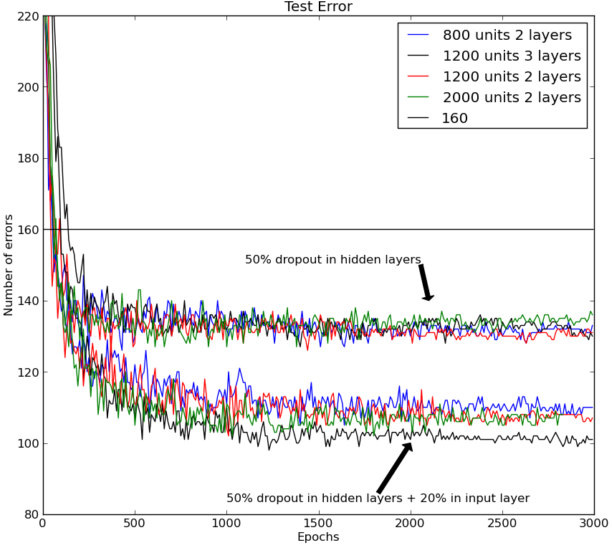
\includegraphics[scale=0.4]{images/dropout.png}
	\caption{source: (Hinton et al 2012)}
\end{figure}

Dropout reduces over-fitting by being equivalent to training an exponential number of models that share weights in reasonable time: there exists an exponential number of different dropout configurations for a given training iteration, so a different model is almost certainly trained every time. At test time, the average of all models is used, which can be seen as a powerful ensemble method. \\

\clearpage

\subsection{Deep Convolutional Neural Networks}

A convolutional neural network is a deep feed-forward neural network with at least one convolutional layer. A convolutional layer differs from a traditional fully connected layer in that it imposes specific operations on the data before and after the data is fed through the activation functions. These specific operations are taken from the pre deep learning era of computer vision, and are detailed in this subsection. \\

Before diving into the details, a notable point to bear in mind is that these operations impose a prior on the underlying structure of the observed data: translation invariance of the features. Consider the following image of a geranium: a good (albeit complex) feature to classify this image would be the blue flower, regardless of the location of the blue flower. This feature could appear anywhere on the image; therefore, if the network can learn it, it should then sweep the entire image to look for it. It is in this sense that the pixel feature is `convolved' over the image. \\

\begin{figure}[h!]
	\centering
	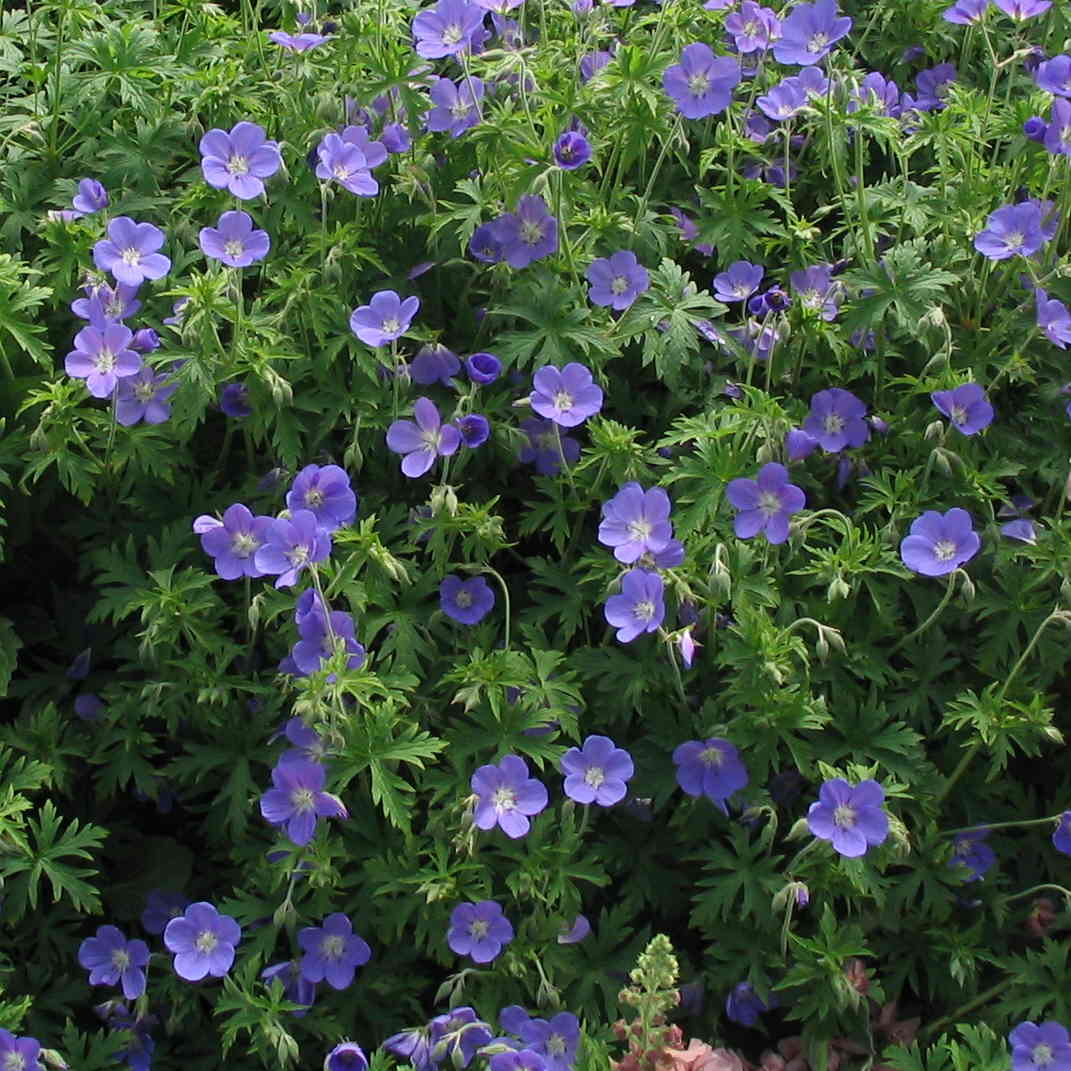
\includegraphics[scale=0.2]{images/geranium.jpg}
	\caption{LeNet7 architecture: each square is a kernel}
\end{figure}

The following subsection is an explanation of the computation that occurs in a convolutional layer. Users of Convolutional Neural Networks for classification tasks are sometimes accused of using them as a black box without understanding them; therefore, this section is crucial in establishing an in-depth understanding of how they function and why they might be so successful. \\

The architecture from (Krizhevsky et al 2012)'s record-breaking image classification model -- which has since been frequently reused for natural scale image classification tasks with CNNs \cite{rectifier} \cite{goodfellow_street_view} \cite{decaf} \cite{fergus_tutorial} \cite{colah} \cite{zeiler_fergus} \cite{transfer-learning} \cite{caffe-website}  -- is summarised below. The softmax layer and fully connected layers having already been covered in section 3, the subsequent subsection is explains what remains: the inner workings of a convolutional layer. \\

\begin{figure}[h!]
	\centering
	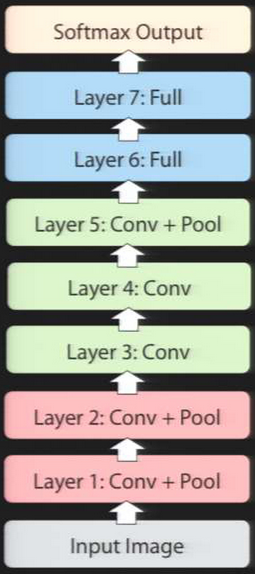
\includegraphics[scale=0.3]{images/alexnet_architecture_simple.png}
	\caption{Architecture of CNN from (Krizhevsky et al 2012)}
\end{figure}

A\footnote{A large portion of the content from this subsection on explaining the operations in a convolutional layer is heavily inspired from Prof Robert Fergus's NIPS 2013 tutorial \cite{fergus_tutorial}.} convolution layer has a pixel feature i.e. filter which is convolved over the entire image, followed by a non-linearity, followed by a spatial feature, optionally followed by a normalisation between feature responses. This structure is similar to hand-crafted features in computer vision such as SIFT and HOG \cite{SIFT}. The key difference is that each operation is learned, i.e.\ optimised to maximise performance on the training set. \\

\subsubsection{Pixel Feature}

A\footnote{This subsection on explaining sliding kernels is heavily inspired from a blog post by Christopher Colah \cite{colah}.} $k \times k$ pixel feature, also referred to as sliding kernel or sliding filter, is defined as a $k \times k$ matrix $\mathcal{W}$ that is applied to $k \times k$ windows $\mathcal{X}$ of the image by performing  the matrix dot product $\sum_{i=0}^{k-1} \sum_{j=1}^{k} x_{ij} \cdot w_{ij}$. An example with $k=3$ is shown below.

\begin{figure}[h!]
	\centering
	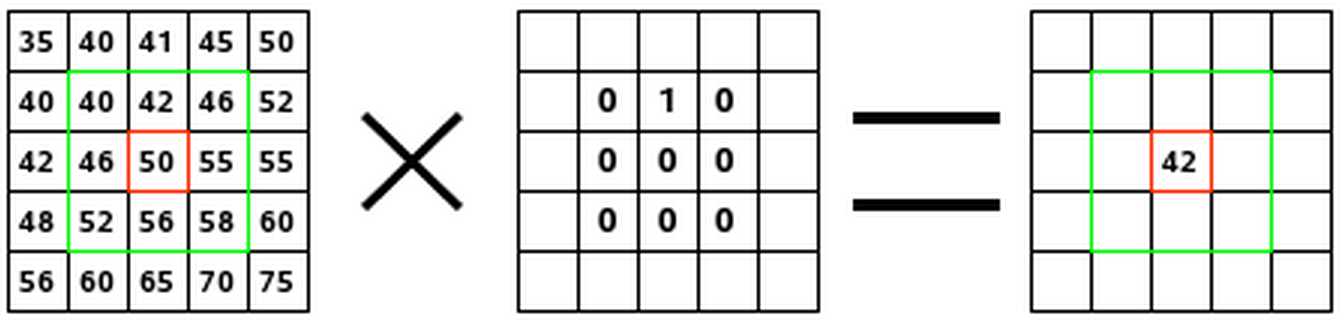
\includegraphics[scale=0.3]{images/window_x_kernel.png}
	\caption{Selecting a pixel window and applying a kernel to it (source: convmatrix Gimp documentation)}
\end{figure}

Notice that this is equivalent to the vector product component of the generic neural network inputs combination $z = b + \sum\limits_{i=0}^{n-1} x_{i}\cdot w_{i}$, where the pixel matrix representation of the entire image is flattened into the vector $\textbf{x}$, the weights of the kernel are flattened into a portion of the weight vector $\textbf{w}$, and all weights corresponding to a pixel that is not part of the window are set (and fixed) to zero. Fixing many weights to zero imposes a strong prior on the network and significantly reduces the function space, making it easier to search for good functions. The crucial aspect of CNNs is that, by representing these kernels as weight vectors of the network, a large set of optimal features can be learned over the dataset without having to handcraft them, as were for example SIFT and HOG \cite{SIFT}. \\

By convolving the kernel over the image, one obtains a feature response map (referred to as kernel map in computer vision jargon):

\begin{figure}[h!]
	\centering
	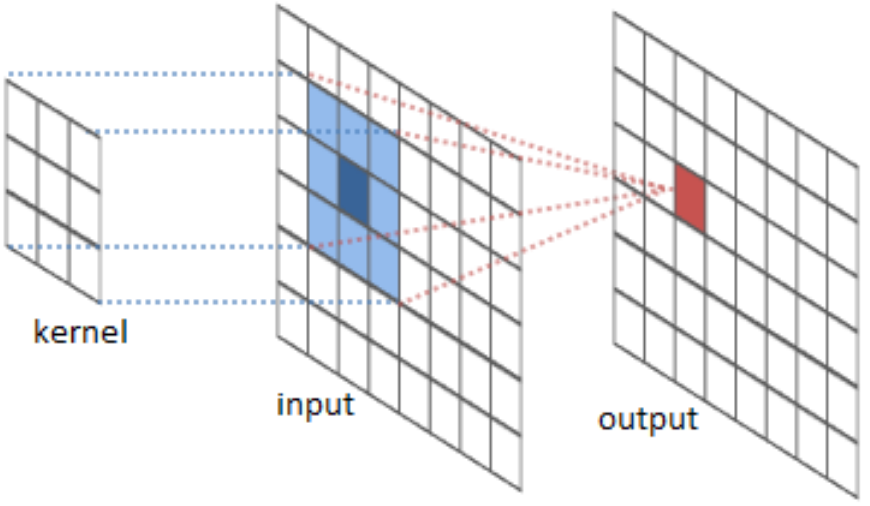
\includegraphics[scale=0.3]{images/kernel_map.png}
	\caption{Producing a kernel map (source: River Trail documentation)}
\end{figure}

Another advantage of such pixel features is that one can make sense of what the weights represent i.e.\ what the network is learning. For example, consider the following image, sliding kernel and resulting kernel map:

\begin{figure}[h]       
    \fbox{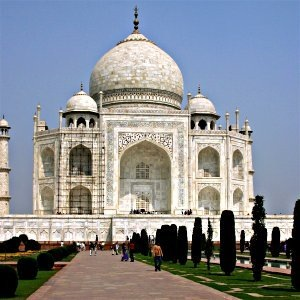
\includegraphics[scale=0.9]{images/taj_mahal.jpg}}   
    \hspace{30px}
    \fbox{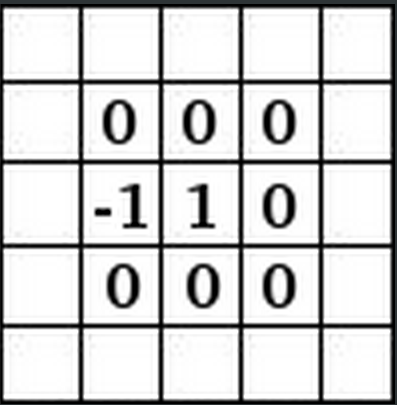
\includegraphics[scale=0.15]{images/kernel_edge_enhance.png}}
    \hspace{30px}
    \fbox{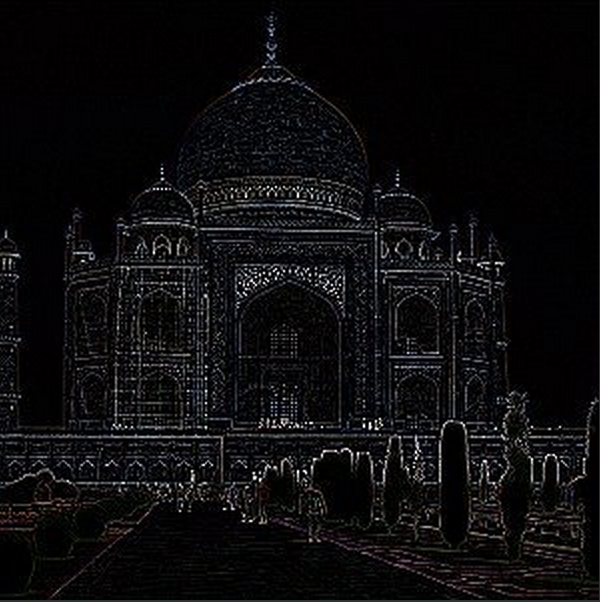
\includegraphics[scale=0.23]{images/kernel_edge_enhance_result.png}}
    \caption{Image, kernel and resulting kernel map (source: convmatrix Gip documentation}
    \label{materialflowChart}
\end{figure}

A zero value is obtained when pixel $(1,0)$ and pixel $(1,1)$ have the same value, which is likely to be the case, hence why most of the kernel map is black. The dot product is maximised when pixel $(1,0)$ is of a much lower value than pixel $(1,1)$, which occurs most often when the window is on a vertical edge separating a dark region to the left from a light region to the right. Therefore, an intuitive representation for the kernel matrix is the pixel window below \footnote{the pixel representation indeed has more pixels than the kernel has entries. but one can see that the dot product is maximal when the kernel is applied in the upper middle area of the pixel representation}, which has become a popular way of representing `deep learning [computer vision] features' \cite{zeiler_fergus}. One therefore realises that this feature visualisation technique does not show a set of weights learned by the network, but the pixel window which maximises the dot product between them and the set of learned weights.

\begin{figure}
    \centering
    \begin{minipage}[b]{\textwidth}
      \begin{subfigure}{.5\textwidth} 
        \centering
        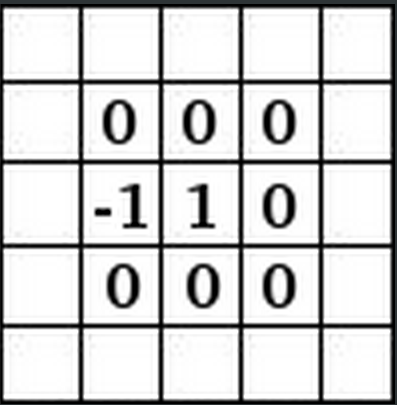
\includegraphics[scale=0.15]{images/kernel_edge_enhance.png}
        % Add \par\vspace*{20pt} here and...
        \caption{Kernel}\label{fig:2a}
      \end{subfigure}%
      \begin{subfigure}{.5\textwidth} 
        \centering
        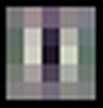
\includegraphics[scale=0.4]{images/kernel_edge_detector.png}
        % ...here to lower the subcaptions and...
        \caption{(Approximate) intuitive representation}\label{fig:2b}
      \end{subfigure} \par \vspace*{20pt} % ...remove them from here
    \end{minipage}%
\end{figure}

In order to impose convolution i.e.\ application of the same kernel over the entire image, the learning rule \eqref{eqn:learning_rule} given in section 3.3.2 is modified to:

\begin{equation}
 w_{i,t+1} = w_{i,t+1} + \tau \cdot \sum_{j \in \mathcal{K}}	\frac{\partial{E}}{\partial{w_{j,t}}}
\label{eqn:conv_learning_rule}
\end{equation}

Where $\mathcal{K}$ is the index set for all neurons intended to apply the kernel to a different location on the image. This learning rule ensures that the i-th weight of all such neurons are updated by the same value. At initialisation, each i-th weight is also set to the same value. The result is that the weight vectors for all these neurons are identical throughout training, i.e.\ the corresponding kernel is convolved over the entire image. \\
 
\subsubsection{Non-linear Activation}

Going to be applied to each output of the feature map independently, no interaction between the elements in the feature map. it's here because the kernel convolution is a linear operation, and we want non-linearity. the currently best performing known activation is the ReLU (extensively discussed in section 5 of the report). an important element is the bias, which in the case of the ReLU allows to choose the input threshold at which the neuron turns off. the bias is the same across every neuron of the feature map. \\

\subsubsection{Pooling aka Spatial Feature}

Take a $k \times k$ spatial neighbourhood of the feature map, and compute some summary statistic over it (average or max). The most common operations are average and max. Max is the currently best performing pooling operation, and this is theoretically backed by (Boureau et al 2010). The intuition behind the theoretical analysis can be illustrated by the following example: given a pixel feature, a $3 \times 3$ spatial neighbourhood to pool over and two different images, consider the case where image A has the feature present in a single location of the neighbourhood (activation output is 1 for this location, 0 elsewhere), whereas image B does not (activation outputs are 0 across all locations of the neighbourhood). Since the feature map seeks to discriminate inputs based on the presence of its feature, we would wish for the pooling operation to assign starkly different values to images A and B. With max pooling, A receives pooled value 1 and B receives pooled value 0; with average pooling, A receives a mere $\frac{1}{9}$ and B receives 0. Therefore, max is better. \\

In general, a potential advantage of average over max is that it conserves more information; on the other hand, it will dilute an activation that is strong in a single location of the given neighbourhood and weak in the others. In the worst case, opposing activations will cancel each other out, and result in the pooled value as that for a neighbourhood with zero activations (however, note that this does not occur with ReLUs since they are not antisymmetric). \\

The key contribution of max pooling is robustness to noise and invariance to small transformations, since the same max pooling output is obtained regardless of where in the neighbourhood the maximal feature activation occurs, and regardless of what is present elsewhere in the neighbourhood. At higher convolutional layers, the resulting invariance can be spectacular. For example, below are kernel maps for a certain feature of the 5-th convolutional layer of a net from (Zeiler and Fergus 2013) \cite{zeiler_fergus}, computed for 9 different input images from the same class ("human"), which obtain similar pooled activation values. One may be struck by the fact that they receive similar pooled activation values, since one can tell that the similarities between the kernel maps are complex and would be difficult to describe in terms of "small transformations". \\

\begin{figure}
    \centering
    \begin{minipage}[b]{\textwidth}
      \begin{subfigure}{.5\textwidth} 
        \centering
        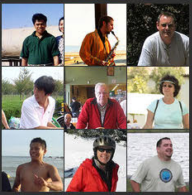
\includegraphics[scale=0.7]{images/high_level_invariance_orig.png}
        % Add \par\vspace*{20pt} here and...
        \caption{9 input images of the "human" class}\label{fig:2b}
      \end{subfigure}%
      \begin{subfigure}{.5\textwidth} 
        \centering
        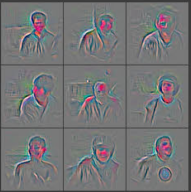
\includegraphics[scale=0.7]{images/high_level_invariance.png}
        % ...here to lower the subcaptions and...
        \caption{9 corresponding kernel maps with similar pooling outputs}\label{fig:2a}
      \end{subfigure} \par \vspace*{20pt} % ...remove them from here
    \caption{source: (Zeiler and Fergus 2013)}
    \end{minipage}%
\end{figure}

By stacking n convolutional layers with $k \times k$ pooling operations, the output of a pooling neuron on the n-th layer has a $k^n \times k^n$ receptive field over the image. Choosing the number of convolutional layers is therefore a matter of finding n such that $k^{2n}$ equals the dimensionality of the input set, i.e.\ such that the highest convolutional layer can recognise complex features spanning the entire image, which is when total translation invariance is achieved. \\

\subsubsection{Contrast Normalisation}

Pick a single location of the output, have a little spatial neighbourhood around that, and perform the linear transformation on all the output values in this neighourhood that results in the best fit of a zero mean, unit standard deviation Gaussian. These transformations are used in image processing to handle images where contrast intensity varies across different areas of the image. The neighbourhood can be defined geographically over isolated kernel maps, or across kernel maps. This normalisation achieves a rescaling of the features at each layer. For example, if in a certain neighbourhood output values are all low and in another neighbourhood all output values are high, this may be due to photographical factors (e.g.\ different expositions to light) which have nothing to do with the underlying objects of interest; local contrast normalisation will pull up the values of the low value neighbourhood and reduce those of the high value neighbourhood to put both neighbourhoods on an equal footing for the next layer to receive unbiased data. \\


\subsection{Local vs Global Optimisation}

Gradient descent is a local optimisation algorithm in that it ends when the first local minimum has been met. This is a major shortcoming when the error surface -- defined by the deep architecture and the dataset -- has minima that vary significantly in depth. However, empirical evidence suggests that this is not the case for convolutional neural networks \cite{DL-book}. Given a sufficiently large labelled dataset, the performance difference reached by a CNN trained with backpropagation with and without unsupervised pretraining on another dataset is negligible \cite{rectifier}. 

One can imagine that the requirement of a large enough dataset is to obtain a sufficiently precise approximation of the `true' error surface, i.e.\ the error surface that would be obtained by integrating the gradient over all possible configurations of the class. But the theoretical explanation for depth similarities across local minima remain a mystery. The question was asked by this author to Yann LeCun at a conference for students in Paris on 12th June 2014. The answer was that: 

\textit{`The optimisation is simple because there are results from random matrix theory that seem to suggest that when you build those systems, the function you are trying to optimise is akin to a high degree polynomial on the sphere, with lots of monomials. The properties of the critical points which are saddle points are relatively well analysed by people who have traditionally worked on things like spin glass theory. What is known is that the minima are clustered within a very small narrow band of energies, so if you have a process that's going to find a minimum, it will find one that will be as good as any minimum. The likelihood of being trapped in a bad minimum is small because there are exponentially more good minima than bad ones. Of course, there is an even larger number of saddle points, so you have to figure out how to avoid saddle points; but you don't get trapped by saddle points, you only get slowed down by them`} \cite{labex-bezout}.

No papers regarding this research were found. When the question was reposted to the Google+ Deep Learning community, Yann LeCun answered that \textit{`This work is not yet published. Stay tuned'}.

\clearpage

The objective of the literature review until now has been to serve as a preamble, in order to understand the models which were used throughout the project. The two subsections that follow are more specific and relate to challenges encountered when training classifiers for ControlPoint. The papers discussed were read in an ad hoc manner, so their relevance will become clearer later on in the Experiments sections that bear the same name. Therefore, especially in the case of the class imbalance literature, deeper examination of the papers is left for then. \\

\subsection{Transfer Learning}

Transfer learning consists in initialising the weights of layers of a network to those of dimensionally identical layers of a network trained in a supervised fashion on a similar task. Until 2013, the established approach consisted in transferring the weights of a Deep Belief Net trained (in an unsupervised fashion) on a `source' unlabelled dataset \cite{microsoft-book}. However, the 2014 paper "CNN Features off-the-shelf: an Astounding Baseline for Recognition" by Razavian et al shows that transferring the weights of OverFeat -- a model that is identical to AlexNet in architecture and winner of the ILSVRC 2013 challenge \cite{transfer-learning} -- to initialise the training of classifiers on 11 well known computer vision recognition tasks, establishes state-of-the-art results on 10 of them\cite{off-the-shelf}.

The transfer models are obtained by training linear Support Vector Machines on the feature space defined by the bottom seven layers of OverFeat. The subsection below is therefore a rapid overview of the mathematics that underlie the training of a linear SVM. 

\subsubsection{Linear Support Vector Machines}

The hinge loss learns the linear decision boundary for classifying inputs which minimises the number of mis-classifications and maximises the \textit{margin}, which is defined as the smallest distance between the decision boundary and any of the training cases \cite{ML-book}. Mathematically, the decision boundary is the hyperplane defined by the equation $\textbf{w}^T \phi(\textbf{x}) + b = 0$ where the parameters $\textbf{w}$ and $b$ are solution to:

\begin{equation}
arg\max\limits_{\textbf{w},b}\{\frac{1}{||\textbf{w}||} \min\limits_{1 \leq i \leq n}\{t_i (\textbf{w}^T \phi(\textbf{x}_i)+b)\}\}
\end{equation}

Where $n$ is the size of the training set, $t_i \in \{-1,1\}$ is the label for training case $\textbf{x}_i$, $\phi$ is the function represented by the first seven layers of the transferred model, and $\textbf{w},b$ define the linear computation that produces classification predictions, namely: \\

$\textbf{w}^T \phi(\textbf{x}) + b > 0 \rightarrow $predicted label value is 1 \\
$\textbf{w}^T \phi(\textbf{x}) + b < 0 \rightarrow $predicted label value is -1 \\

The intuition behind the mathematical formula is that the distance from a point $\textbf{x}_1$ to a hyperplane defined by the equation $h(\textbf{x}) = \textbf{w}^T \phi(\textbf{x}) + b = 0$ is given by $\frac{|h(\textbf{x}_1)|}{||\textbf{w}||}$. In the case of classification, when the decision boundary correctly separates the entire trainin set, $|h(\textbf{x}_1)| = t_1 h(\textbf{x}_1)$. $\min\limits_{1 \leq i \leq n}\{t_i (\textbf{w}^T \phi(\textbf{x}_i)+b)\}$ finds the points closest to the decision boundary. 

Solving this optimisation problem with brute force would be intractable \cite{ML-book}, but it can be shown that it is equivalent to the following constrained optimisation problem:

\begin{equation}
arg\min \limits_{\textbf{w},b} ||w||^2 \text{, subject to } \forall 1 \leq i \leq n, t_i(\textbf{w}^T \phi(\textbf{x}_i)+b) = 1
\end{equation} \\


\subsection{Class Imbalance}

\paragraph{Definition}

The literature \cite{imbalance} \cite{maloof} \cite{zhou} \cite{f-measure} has defined class imbalance as the situation where the sample distribution of classes is significantly non-uniform, i.e.\ where there exists a class of significantly smaller size than another. However, as will be seen later, this definition does not necessarily make class imbalance detrimental to learning. A definition for `dangerous class imbalance' will be given with the aim of being the largest set of conditions that are necessary for class imbalance to be detrimental to training classifiers with stochastic gradient descent and standard cost functions. \\

The literature on deep learning with class imbalance was found to be scarce. Zhou and Liu in `Training cost sensitive neural networks with methods addressing the class imbalance problem' (2005) \cite{zhou} experiment with \textbf{under-sampling}, textbf{over-sampling} and \textbf{threshold-moving} to deal with class imbalance, and find threshold-moving to perform best.

`F-measure as the error function to train neural networks' by Pastor-Pellicer et al, 2013 \cite{f-measure}, does not make use of these techniques and instead introduces a cost function for binary classifiers which is the harmonic mean of precision and recall. Deep neural networks are trained on it as well as on the Mean Squared Error for 3 image-cleaning tasks with levels of class imbalance below those experimented with in this report. The image-cleaning task is framed as a classification task where the probability of ink in each pixel of the clean image is to be predicted given the noisy image. MSE as a cost function for training deep neural network classifiers is known to train slower and converge to the same performance as when the cross entropy error is used \cite{coursera}. 

The authors find that `both training techniques perform quite well' on the basis that `a well cleaned image gives good results on both metrics'. This seems to merely state that the error computed on a correctly classified input is low in absolute terms, for both cost functions. An analytical comparison of the cost functions by rescaling input domain and output range, such as the one between softmax cross entropy and hinge loss in (Bishop 2010) \cite{ML-book} and in the previous section, is not included. An empirical comparison of the cost functions by evaluating a model trained on each against a common performance metric such as percentage classification accuracy is not provided either. It appears that this cost function does not deliver significant performance gains.

\clearpage

\section{Analysis 1: ReLU Activation}

\subsection{Motivations}

Differentiable, symmetric, bounded activation functions that introduce a non-linearity smoothly over the entire input domain were the activation units of choice in deep feed-forward neural networks, until Rectified Linear Units were used for CNNs in 2012 \cite{krizhevsky} and found to outperform their counterparts. They make the observations that $f(x) = \tanh x = \frac{1 - e^{-2x}}{1 + e^{-2x}}$ or $f(x) = (1+ e^{-x})^{-1}$ "saturating non-linearities" are slower to train than the $f(x) = max(0,x)$ "non-saturating non-linearity", and report an "accelerated ability to fit the training set", but do not provide any explanations.   \\

\begin{figure}
    \centering
    \begin{minipage}[b]{\textwidth}
      \begin{subfigure}{.5\textwidth} 
        \centering
        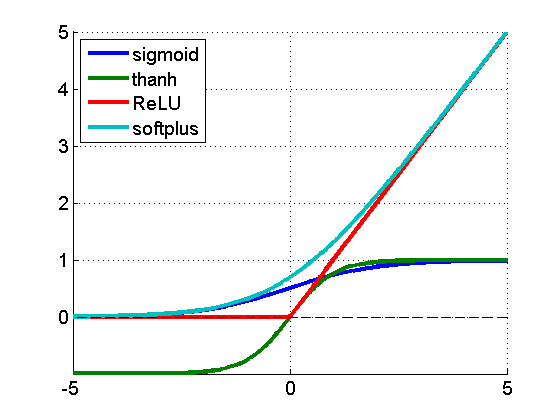
\includegraphics[scale=0.5]{images/activation_functions.png}
        % Add \par\vspace*{20pt} here and...
        \caption{Activation functions}\label{fig:2a}
      \end{subfigure}%
      \begin{subfigure}{.5\textwidth} 
        \centering
        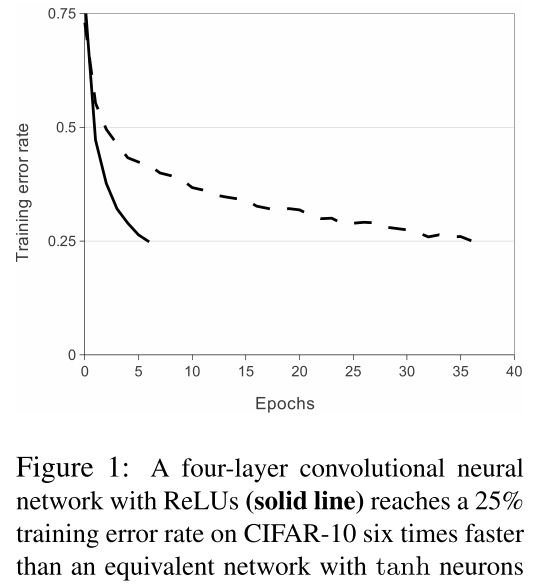
\includegraphics[scale=0.35]{images/ReLU_train_fast.png}
        % ...here to lower the subcaptions and...
        \caption{source: Krizhevsky et al 2012}\label{fig:2b}
      \end{subfigure} \par \vspace*{20pt} % ...remove them from here
    \end{minipage}%
\end{figure}

The importance attributed to non-linearity of activation functions is due to the function space that is spanned by composing such functions as deep neural networks do. If activation functions are linear, the overall network is linear too, and as seen in section 3.2.2, such networks are greatly limited in what they can learn. Therefore, one may wonder whether or how the function space is reduced by using an activation function such as the ReLU that is non-linear only in the neighbourhood of $0$.  \\

(Glorot, Bordes and Bengio 2013) \cite{rectifier} explain that "the only non-linearity in the network comes from the path selection associated with individual neurons being fired or not. [...] We can therefore see the model as an \textit{exponential number of linear models that share parameters}". Since for a certain range of inputs, a ReLU will not fire, one can view the network as selecting different subsets of itself based on the input. Each subset is a linear function, but two inputs which are very close (in the sense of euclidean distance) in the input space might (de)activate different neurons, and therefore be processed by different (linear) functions that output completely different results. In this sense, non-linearity is achieved. \\

\begin{figure}[h!]
	\centering
	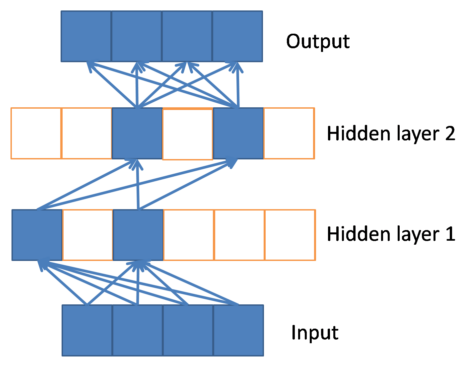
\includegraphics[scale=0.4]{images/ReLU_path_selection.png}
	\caption{ReLU path selection (source: Glorot et al 2013)}
\end{figure}

(Glorot, Bordes and Bengio 2013) also remark that "because of [the ReLU's] linearity, gradients flow well on the active paths of neurons (there is no gradient vanishing effect due to activation non-linearities of sigmoid or tanh units)", but no explanations of enhanced flow or vanishing gradient are given (instead, the paper focuses on the benefits of sparse representations and their greater resemblance to neuron activations in the brain). Another empirical finding of the paper is that "deep rectifier networks can reach their best performance without requiring any unsupervised pretraining". This section of the report is a simple mathematical analysis of backpropagation that conveniently provides an explanation for these points as well as (Krizhevsky et al 2012)'s observations. In the context of building pipe weld classifiers, the motivation for doing is to understand the mechanics of training for the CNNs to be subsequently used. \\

%This may come as a surprising result for several reasons:
%\begin{enumerate}
%\item unlike every other neuron model, they are not $antisymmetric$ ("when its response to the oppposite of a strongly excitatory input pattern is respectively a strongly inhibitory one" \cite{rectifier}), but rather $one sided$ (the response is zero). This drops a prior assumption on how information should be interpreted and transferred between layers.
%\item the angular point makes them non-differentiable at 0, since we have $\lim_{x \to 0^+} \frac{\partial max(0,x)}{\partial x} = 1 $ and $\lim_{x \to 0^-} \frac{\partial max(0,x)}{\partial x} = 0$). But gradient descent depends on differentiating activation functions, so an arbitrary choice needs to be made for $x = 0$. 
%\item 
%\item they are unbounded above, which could increase the difficulty in training the network by making exploding outputs easier to produce.
%\item they are not bijective: $tanh$ is a one-for-one mapping from $\mathbb{R}$ to $[-1,1]$ and $sigmoid$ is a one-for-one mapping from $\mathbb{R}$ to $[0,1]$, therefore information is preserved; ReLU maps all of $\mathbb{R}^-$ to $0$, which loses information.
%\end{enumerate}

%The literature currently does not provide a detailed mathematical explanation for the superiority of ReLU over sigmoid and tanh units in deep neural networks trained with backpropagation. 
%
%(Krizhevsky et al 2012) \cite{krizhevsky} are the first to notice the benefits of ReLU in the context of supervised deep learning (i.e.\ backpropagation). 
%
%
%The authors use evidence from neuroscience to justify the superior performance of the ReLU, namely that "studies on brain energy expense suggest that neurons encode information in a sparse and distributed way", and that the one-sided response of ReLUs introduces "real zeros of activations" which leads to sparse representations of the data in the network. A sparse representation is one in which the vector representation has many zero entries. Sparsity is advocated for four intuitive reasons:
%
%\begin{enumerate}
%\item \textbf{Information disentangling}: an underlying assumption of many high dimensional deep learning classification tasks is that the class is a low-dimensional manifold in a high dimensional space. For example, the face manifold has a number of dimensions equal to the degrees of freedom in which the face can move and change, which might be around 7, but if considered in the space of all 256x256 greyscale images, it lies in a 65,536 dimensional space. If so, then there must exist an information-preserving projection of this space into a 7-dimensional space, which is equivalent to an information-preserving transformation of this space such that any vector of the face manifold has only at most 7 non-zero entries. In this sense, the manifold is disentangled from the many dimensions. By mapping $\mathbb{R}^-$ to $0$, the ReLU encourages sparse representations. 
%\item \textbf{Efficient variable-size representation}: "varying the number of active neurons allows a model to control the effective dimensionality of the representation for a given input and the required precision".
%\item \textbf{Linear separability}: sparse representations are easy to linearly separate, for example by using as a separating condition whether or not the k-th entry is zero. 
%\item \textbf{Distributed but sparse}: this point reassures that sparsity does not come at the expense of a distributed representation, the benefits of which are detailed in section 3.2.2 of this report. Sadly, the paper does provides extensive justification of this point \footnote{a question was posted on the Google+ Deep Learning community on 01/09/2014 asking for clarification, and awaits response}.
%\end{enumerate} 
%
%Although the authors focus on sparsity, they also address points 2 and 5 raised in the motivations: antisymmetric activation can be obtained by combining two ReLUs that share parameters, and the upward unboundedness of the ReLU can be controlled with an $L_1$ regulariser.

\subsection{Mathematical Analysis}

Recall from section 3.3 that the model is trained with backpropagation: each of the weights $w$ are adjusted by $\tau \cdot \frac{\partial{E}}{\partial{w}}$. The choice of activation function modifies $\frac{\partial{E}}{\partial{w}}$; this section looks at how ReLU does so compared to sigmoid or tanh. \\

\subsubsection{How the Gradient Propagates}

It may be useful for intuition to think of $\frac{\partial{E}}{\partial{w}}$ in the context of the gradient travelling through the network. With the following notation:
\begin{itemize}
%\renewcommand\labelitemi{--}
\item $y_{j}$, the output of unit (a.k.a\ neuron) $j$, but also used to refer to the unit $j$ itself
\item $w_{ij}$, the weight of the edge connecting lower-layer neuron $y_{i}$ to upper-layer neuron $y_{j}$
\item $z_{j} := b+ \langle x,w \rangle = b + \sum\limits_{i=1}^k x_{i}\cdot w_{ij}$, the input vector for $y_{j}$
\item $\psi$, the activation function used -- therefore $y_{j} = \psi(z_{j})$ \\
\end{itemize}

The backpropagation algorithm can be formulated as a set of rules for propagating the gradient through the network:
\begin{itemize}
\renewcommand\labelitemi{--}
\item to \textbf{initialise}: $grad \leftarrow \mathcal{C}'(y_{L})$, where $y_{L}$ is the output unit
\item to \textbf{propagate through a unit} $y_{j}$: $grad \leftarrow grad \cdot \psi'(z_{j})$
\item to \textbf{propagate along an edge} $w_{ij}$: $grad \leftarrow grad \cdot w_{ij}$
\item to \textbf{stop at an edge} $w_{ij}$: $grad \leftarrow grad \cdot y_{i}$ \\
\end{itemize}


\subsubsection{An Example}

\begin{figure}[h!]
	\centering
	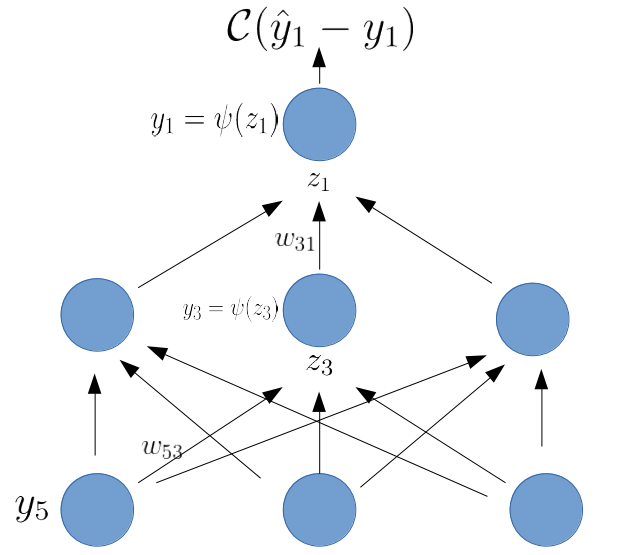
\includegraphics[scale=0.4]{images/gradient_propagates.png}
	\caption{$\mathbb{R}^3 \rightarrow \mathbb{R}$ MLP with 1 hidden layer}
\end{figure}

Given the figure above:
\begin{itemize}
\renewcommand\labelitemi{--}
\item for $\frac{\partial{E}}{\partial{w_{31}}}$: initialise, propagate through $y_1$, then stop at $w_{31}$:
 $ \mathcal{\mathcal{C}}'(y_1) \cdot \psi'(z_1) \cdot y_3$ 
\item for $\frac{\partial{E}}{\partial{w_{53}}}$: initialise, propagate through $y_1$, then along $w_{53}$, then stop at $w_{53}$: \\
 $\mathcal{C}'(y_{1}) \cdot \psi'(z_1) \cdot w_{31} \cdot \psi'(z_3) \cdot y_5$ \\
\end{itemize}

Intuitively, the partial derivative with respect to a weight can be roughly seen as the product of the partial derivative of every component along the path from the weight to the output unit \footnote{this only goes for this simple case where we have one hidden layer and one output node. That is because, if we consider all paths from an input node to an output node, every edge exists in exactly one path. However, if we had more output nodes or more hidden layers, there would exist edges belonging to several input-output paths. In this case, the partial derivative would be the sum across all paths from the weight to some output unit.}. \\


\subsubsection{Vanishing Gradient}

Notice that $\psi'(z_1)$ is a factor in both partial derivatives. Now, consider the derivatives of the tanh and sigmoid functions: 

\begin{equation}
tan'(x) = 1 - tan^2(x)  \\
\end{equation} \\
\begin{equation}
sigmoid'(x) = \frac{1}{1 + e^{-x}}
\end{equation} \\

The formulae do not lend themselves to intuition, but their graphical representation given below does \footnote{both are the same up to a scaling factor, therefore only one is given.}. Such functions are called "saturating" by (Krizhevsky et al 2012) because, when the input is high in absolute value, the derivative approaches zero. In the context of backpropagation, this means that a tanh or sigmoid unit that is "heavily activated" during the forward pass will strongly reduce the gradient as it propagates through it during the backward pass. Moreover, this will affect the partial derivative of every weight that lies behind the unit in some input-output path. As a result, during training it becomes slow to alter any such weight when the unit's weights are on average high in absolute value. This difficulty increases with the depth of the network, since in order to reach a weight that is low down in the network, the gradient must propagate through a higher number of units, so its probability of vanishing increases. This is consistent with empirical findings \cite{DL-book}. \\

\begin{figure}[h!]
	\centering
	\begin{subfigure}{.5\textwidth}
  		\centering
		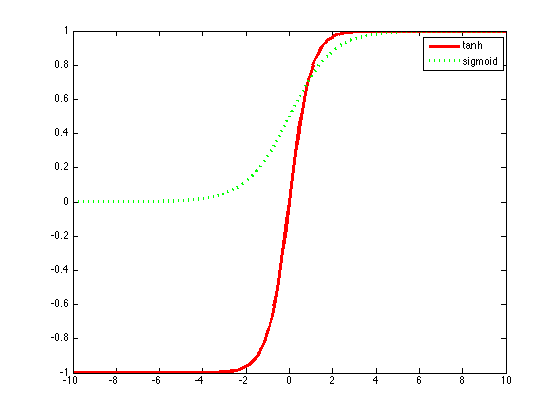
\includegraphics[scale=0.4]{images/tanh_sigmoid.png}
		\caption{tanh and sigmoid functions}
	\end{subfigure}%
	\begin{subfigure}{.5\textwidth}
  		\centering
		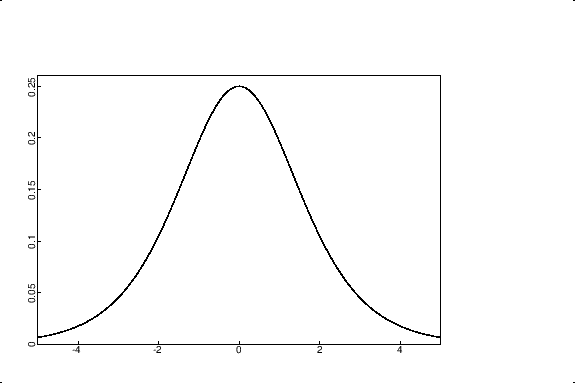
\includegraphics[scale=0.4]{images/logistic_derivative.png}
		\caption{derivative for the tanh and sigmoid}
	\end{subfigure}
\end{figure}

One may argue that a unit which has learned a feature that is useful for the task is one that is heavily activated for certain inputs. Therefore, it is a good thing that it becomes rigid to change. However, traditional training of deep neural networks occurs by first randomly initialising the weights. At first, it is therefore unlikely that a unit is heavily activated because it is a detector for a meaningful feature. If the network is built on saturating activations, such non-meaningful features will be harder to get rid of. \\


\subsubsection{Impact of the ReLU}

On the other hand, the derivative of the ReLU is given by:

\begin{equation}
ReLU'(x) = \begin{cases} 1 & \mbox{if } x > 0\\ 
				  0 & \mbox{otherwise} \end{cases}
\end{equation} 

Which means that for any positive input, the gradient will \textit{not be modified} when propagating through the unit. It is in this sense that "gradients flow well on the active paths of neurons". On the other hand, for any negative input, the gradient is brought to zero i.e.\ halted from propagating altogether. This could be cause for concern, because if the weights of a ReLU are initialised to values that, given the distribution of the input, always lead to a zero activation, then there is no way of modifying them, and the neuron is effectively a useless component of the network. When training, one should therefore take care to choose a sufficiently high positive value for the neuron's initial bias \footnote{This makes the bias $b$ in $z = b + \langle x, w \rangle$ a crucial element of a neural network, despite them being conventionally excluded from graphical representations}. On the other hand, halting the gradient in this regard has the intuitive benefit of reducing the areas of the network to which it propagates, and focusing it on the areas responsible for the error. If one goes back to the vision of a deep sparse rectifier network as an exponential number of linear models, gradient halting enables the training of a smaller network at every iteration. \\

Since vanishing gradient makes it slow to get rid of non-meaningful features that receive heavy activations, this provides an explanation for why "deep sparse rectifier networks can reach their best performance without requiring any unsupervised pre-training", which initialises the weights of the network to features capable of reconstructing the data. It also explains (Krizhevsky et al 2012)'s observations that ReLU networks train faster. By providing a clear mathematical explanation to the main empirical findings regarding deep sparse rectifier networks, this report would argue that the ability of ReLU to enable gradients to "flow well" is the key reason for their success. \\

A final remark concerning ReLUs is that they reduce the computation in both forward and backward passes by turning off a number of neurons and by not interfering with the gradient as it propagates through a unit. \\

\clearpage

\section{Analysis 2: Early Stopping}

Early stopping is a form of regularisation to prevent overfitting. It makes use of cross validation: separating the dataset into a training set, a validation set and a test set. The model's parameters are optimised with respect to the training set (i.e.\ backpropagation is run on the training set only), but are considered optimal at the point which minimises the model's error on the validation set. \\

But maybe be taken for granted but is in fact shocking is that when learning a DNN with backpropagation and first order gradient descent, the time series of the validation error always assumes a strictly convex curve (bar some noise). In other words, the validation error has a unique minimum, is strictly decreasing before it, and strictly increasing afterwards. It presents the simplest most convenient shape possible. This is what enables the straightforward strategy of early stopping: (write this as a little algorithm to make it look more classy) while validation error is decreasing, train. \\

One may wonder why the validation error time series is shaped so: why is it not more random? A theoretical and intuitive answer may lie in the optimisation algorithm that is used, first order gradient descent.

\paragraph{Gradient Descent}

Gradient descent consists in finding the weights of the model that locally minimise the model's error. Therefore, if we consider $E : \mathbb{R}^n -> \mathbb{R}$ to be the error function (also referred to as surface) which to a set of $n$ parameters associates the model's error, then the problem can be reformulated as finding the minimum of $E$. 

(erase this?) In the optimisation literature, $E$ is assumed to be strictly convex, because this is the necessary and sufficient condition for gradient descent to be a globally valid algorithm. 

For the sake of providing mathematical intuition as to why early stopping and validation error behave the way they do, assume that $E$ is of the form $E(x) = \frac{1}{2}x^T Ax - b^T x$, where $A$ is an $n \times n$ positive definite matrix and $b$ is a vector. (For 
$ w_k = ( \sum_{t=0}^{T} (I - A')^k)b'$ where 


Combine your intuition with the stuff from that conference, about gradient descent and extra polynomial order.

I've been thinking about it in terms of early stopping. early stopping seems really neat in that it first learns patterns that generalise and then eventually learns patterns that don't generalise, which is when we stop training. I was wondering why  it works so nicely, and thought this inverse approximation formulation of grad descent makes it look like you're adding ever higher order polynomials as you go along. so maybe what's happening is that you're not learning first the patterns that generalise per se, but rather the simplest patterns (that can be fitted with low order polynomial), and as you go along, increasingly complex ones. if you have a large enough dataset the patterns that don't generalise are going to be really complex and require really high order polynomials to fit them, hence why overfit only takes place later.

\clearpage

\section{Experiments 1: Simple Clamp Detection}

\subsection{Motivations}

Clamp detection was suggested by ControlPoint as a simple test run for training a CNN on their dataset. Since computer vision had never been attempted on ControlPoint's dataset, there was no benchmark from which to evaluate the difficulty of the task. The test run was seen as a way of estimating the difficulty, in case the task would turn out to be too ambitious for the scope of the MSc project. Clamp detection was advised on the intuitive basis that, since clamps are large objects, they would be easy to see. 

\subsection{Implementation: Cuda-Convnet}

Due to its success and frequent re-use \cite{rectifier} \cite{goodfellow_street_view} \cite{decaf} \cite{fergus_tutorial} \cite{colah} \cite{zeiler_fergus} \cite{transfer-learning} \cite{caffe-website}, the network architecture from (Krizhevsky et al 2012), often referred to as AlexNet, was chosen for this task (and throughout most of the project).

Cuda-Convnet is an open-source GPU implementation for training deep convolutional neural networks with stochastic gradient descent, written in CUDA C++ and python by Alex Krizhevsky. GPU implementations enable twenty-fold speedups\cite{soumith-benchmark} in training time. Knowledge of its use existed prior to this project since it had already been used for a group project. A shortcoming with the API is that it expects data in the form of batches consisting of numpy arrays of stacked jpg values in matrix format with RGB values split across, and a dictionary of labels and metadata. Python programs were written to achieve this and extract training data from the log files and plotting it. By re-using code written during the group project, the additional code needing to be written was limited to approx.\ 400 lines. The hardware used for training the network was an nVidia GeForce GTX 780 with 4GB RAM, which enables a twenty-fold increase in training speed compared to the CPU. 

\subsection{Experimentation}

Training occurred over the 113,865 image Redbox dataset only, to exclude domain change as a potential reason for weak performance if it were to occur. The task consists in learning three classes: `No Clamps Used', `Photo Does Not Show Enough Of Clamps', and `Clamp Detected' -- which in fact is the default class: an image belongs to it if none of the two mentioned flags have been raised. Time series for training and validation errors were extracted, but not the test error, since it serves no purpose in training the model. 

The error being computed and minimised by Cuda-Convnet is the negative of the log probability of the likelihood function:
\begin{equation}
-\frac{1}{n}\sum\limits_{i=1}^n log(f(W|x_i))
\end{equation}
Where f is the learned function, a.k.a\ the model i.e.\ the neural network. This is also known as Maximum Likelihood Estimation; therefore backpropagation converges to the parameter values that maximise the joint likelihood of the training data. It can be shown that this is equal to the cross entropy of the softmax layer's output \cite{DL-book}. This is discussed in greater length in the experimentation section of Task 3 on class imbalance. 


\subsubsection{Non-Converging Error Rates}

Training produced worrying results: none of the models trained showed signs of learning anything. The below plot of the training and validation errors covers 11 of the 44 epochs over which the model was trained, which amounts to two consecutive days of training. The errors display no trends, and this extends to all 44 epochs.

\begin{figure}[!h]
	\centering
	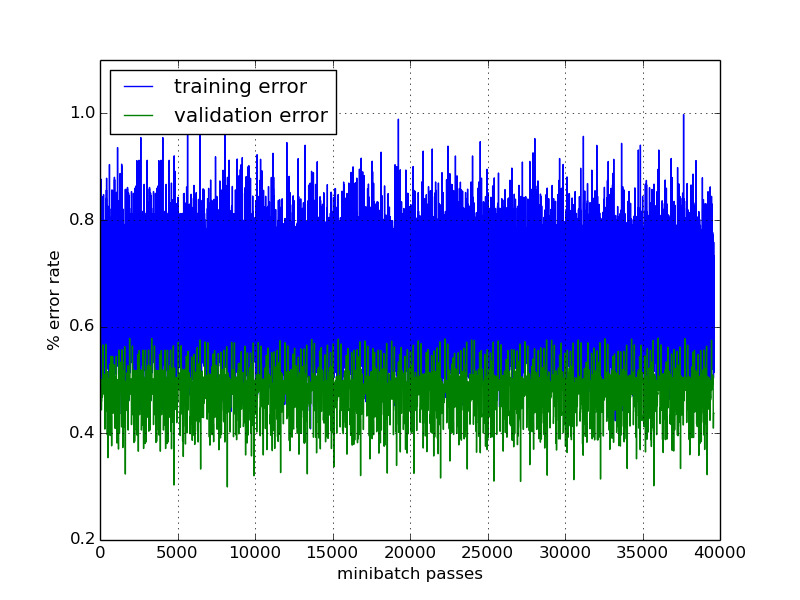
\includegraphics[scale=0.5]{images/test_run.png}
	\caption{Test Run Training Results}
\end{figure}

These results were confusing: the fact that the training error does not converge to zero means that the model is unable to perfectly fit the training set. This should be impossible, since the 60 million parameters of AlexNet make it a very powerful model\footnote{powerful as an approximator, i.e.\ as a `fitter to the data'.} for which (Krizhevsky et al 2012) report overfitting to be `a significant problem', even on the 1000 class, 1.3 million image dataset of the ILSVRC 2012 competition. It makes no sense that the same model would fail to fit a 3-class, 113,000 image dataset.

Moreover, with backpropagation, the network parameters are guaranteed to converge \cite{DL-book} since gradient descent will update weights by zero values once the error-weight partial derivatives are all zero. Such a point in the parameter space exists if there is a local minimum in the error surface at this point. If so, then gradient descent is guaranteed to reach a minimum: intuitively, if one is in a mountain range, then by walking downhill, one is bound to reach some morsel of flat ground at some point. Once the parameters have converged, the model is fixed, so its error is expected to be similar across random samples of the training and validation sets. In this case, the persistent high amplitude of the training and validation errors means that the error is heavily changing all the time.

A number of potential explanations for the high amplitude of the error rates were considered:
\begin{itemize}
\item The learning rates are too high: the minimum keeps getting 'overshot', the weights move endlessly around the rims of a bowl on the error surface\footnote{This interpretation was supported by the Google+ community when the plots were posted.}.
\item The dropout rate is too high: since neurons are randomly dropped at every iteration, a different model is tested every time. The errors correspond to partial derivatives of different models every time, so the amplitude is high. 
\item The number of parameters is too high: AlexNet contains 60 million parameters, far more than than the number of training cases, so collinearities between the parameters cannot even be broken, and most of them are rendered useless.
\item The error rates are not computed correctly.
\item Class imbalance: with 90\% of the data belonging to the same class, there is not enough information about the `No Clamps Used' and `Photo Does Not Show Enough of Clamps' classes to be able to learn features for them.
\item Mislabelled data: the images were not tagged correctly, too many members of one class appear in the other and vice versa, so nothing can be learned.
\end{itemize}

The learning and dropout rates were modified to no avail. (Jarrett et al 2009) report successful training of networks for which `the number of parameters greatly outstrips the number of samples'.

\subsubsection{Increase Validation Error Precision}

If the set of images that the validation error is computed against varies from one iteration to the next, then the variations in validation error are not solely explained by the changes in the model parameters; they may also be due to changes in the validation set. Secondly, precision increases with the size of the set. Therefore, by computing the validation error on a larger and unchanging sample of images, one obtains stable, more precise measures that truly reflect what the model is learning. 

\begin{figure}[h!]
	\centering
	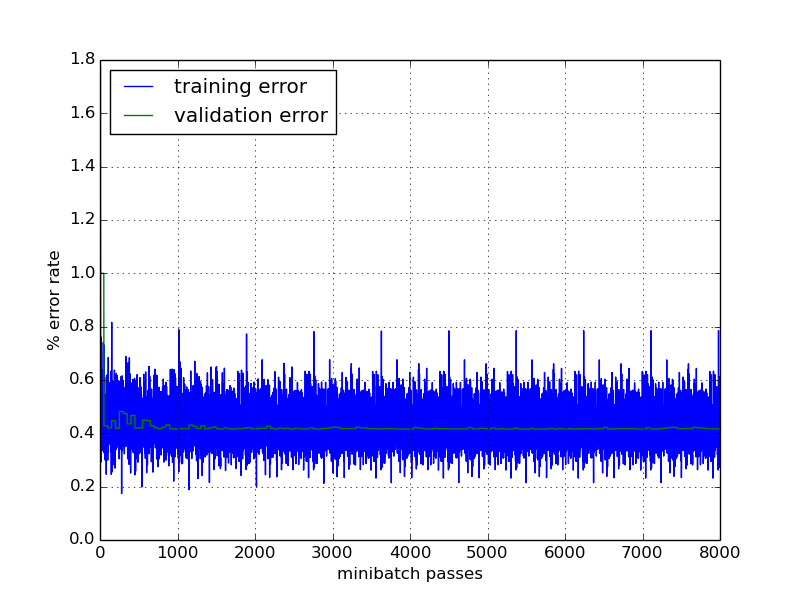
\includegraphics[scale=0.5]{images/increase_test_precision.png}
	\caption{Test Run with validation errors computed over an unchanging set}
\end{figure}

With better validation error measures, one notices that the validation error is flat throughout most of training, indicating that little is learned. There is some movement during the first thousand iterations, suggesting in fact that backpropagation converged within 1000 iterations, which is highly rapid compared to similar tasks \cite{decaf} \cite{fergus_tutorial} cite{transfer-learning} \cite{caffe-website}. One may be tempted to conclude that the model is able to learn only very little.


\subsubsection{Periodicity of the training error}

What remains striking and unexplained is the high amplitude of the training error, and its refusal to converge to zero. Another intriguing aspect is its periodicity: its period corresponds to the number of mini-batches in an epoch. Since the same error is obtained on a mini-batch from one period to the next, the network parameters are therefore not changing from an epoch to the next. Therefore, backpropagation does indeed converge: it does so within a mere 1000 mini-batch passes, at which it attains a local minimum. At this point, the training error has not reached zero; therefore, the model is stuck in a poor local minimum. This is unusual for deep convolutional neural nets, which unlike deep fully connected neural networks are known for being easy to train i.e.\ not getting stuck in poor local minima \cite{DL-book}\footnote{Members of the Google+ Deep Learning community who were interacting on the thread were reluctant to believe that AlexNet could be stuck in a poor local minimum}. 

%Plateau hypothesis: on the image I show only 10 epochs, but I trained it for 44 epochs and the periodicity extends all the way. When you were experiencing plateaus, did they stretch over more than 1 epoch? because to me, this periodicity suggests roughly the same gradients are repetitively being computed at the same locations on the error surface, so no good keeping on going. 
%
%Learning rate hypothesis: so you are suggesting that the minimum keeps getting overshot. But 0.0001 learning rate is already very small no?
%
%I guess another possibility is that I'm zigzagging in a very tight bowl, but seems unlikely it would go on for as long as 40 epochs?\\
%
%Francis Quintal Lauzon: I trained on much larger (though highly correlated) dataset so I never trained for 44 epochs.  I did use learning rate of the same magnitude you are using and still, reducing it after a plateau does help (in my experience).  If you are using momentum, you also might want to reset any momentum to zero after facing a plateau (this might helps as well).\\
%
%
%\paragraph{Alter Momentum}
%
%What is momentum for?
%
%the intuition (maybe wrong): if a smaller learning rate and zero momentum could help you deal with a plateau, it means that moving in very small steps is better. but if a plateau is a continuous flat surface, then surely a smaller step will take you longer to reach the other side? 
%on the other hand, if you're in a very tight and stretched bowl, or if there's a very narrow ditch surrounded by a plateau, then the smaller step will help?
%
%\subparagraph{Increase}
%
%Is that used to get past the local minimum? Or is it used to rush past a plateau?
%
%\begin{figure}[h!]
%	\centering
%	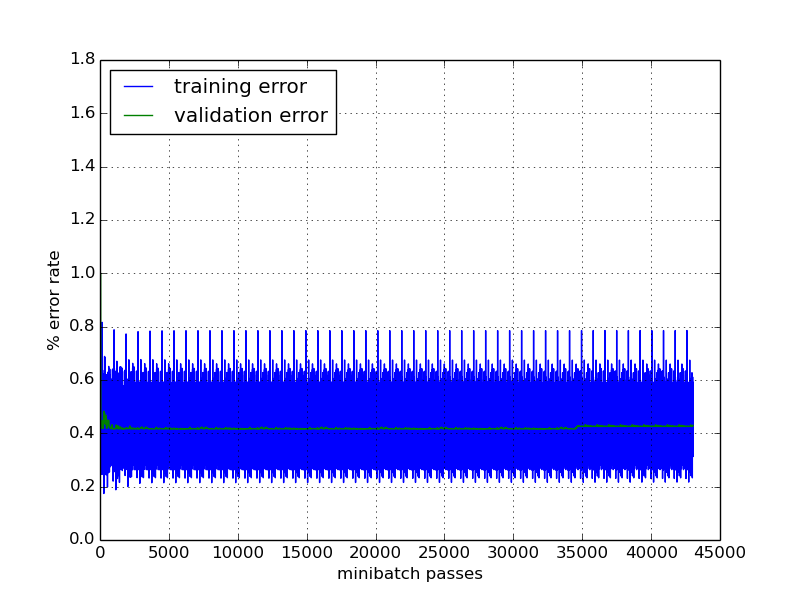
\includegraphics[scale=0.5]{images/raise_momentum.png}
%	\caption{test and validation error rates for clamp detection after raising momentum}
%\end{figure}
%
%Barely noticeable change in train error: still periodic, slightly different shape of period. Slight increase in test error though. Can interpret that weight updates are slightly less optimal since they don't follow the direction given by the gradients, since there's this extra momentum factor, which is bigger.
%
%\subparagraph{Decrease}
%
%Because Francis Quintal Lauzon says so. But does he mean to reduce it once you're done with the plateau?
%
%\begin{figure}[h!]
%	\centering
%	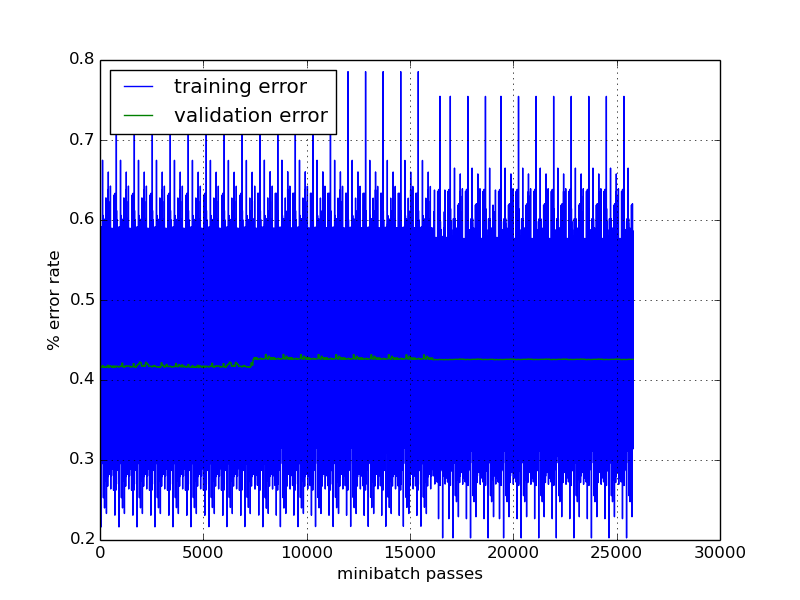
\includegraphics[scale=0.5]{images/change_momentum.png}
%	\caption{test and validation error rates for clamp detection after setting momentum to zero}
%\end{figure}
%
%The training error decreases a little on average (would be good to assert this statistically). Once again, because momentum is not 	distorting direction of descent.
%
%The test error stops to jitter completely. So the tiny pulses observed during convergence (i.e. between 5000 batches and 35000) were caused by momentum. I guess it's the result of going upslope a bit just in case there's a better minimum nearby. Could be interesting to put a stupidly high momentum like 1.5 to double check that jittering indeed gets even bigger. Who knows, this might settle the network in another minimum. 
%
%
%\paragraph{Reduce Learning Rate}
%
%$train_output.txt$ contains data to plot this. Good to put it in to show that you have checked everything meticulously, and to show that it's evidence for the hypothesis of stuck in corner solution.

%I played around with momentum and the learning rate, which typically help to deal with plateaus, tight bowls, and poor local minima. (you can see it on the graph, the test error jitters a bit more, and then becomes completely constant, and the amplitude of the training error varies a bit). It didn't help.


\subsubsection{Poor, Sampling-Induced Corner Minima}

An intriguing aspect is that the 0.419515 validation (logprob) error that the model converges to corresponds to a 10.791\%  error rate, which is the proportion $\frac{12,287}{113,865}$ of Redbox images that belong to the majority class `Clamp Detected'. Furthermore, the error rate on each batch was verified to correspond exactly the proportion of non majority class images within the batch. For example, batch 280 is the best performing batch of the entire set, obtaining 0.315\% error rate at every epoch after model convergence, which is the proportion of `No Clamp' or `Photo Does Not Show Enough Of Clamps' images within; batch 152 is the worst performing and obtains 0.23\% error rate, which is the proportion of non majority class images within. 

Therefore, the reason for why the network converges relatively fast to logprob 0.4 minimum, and stays there, without ever overfitting, is that class imbalance has introduced a `fake' minimum in a `corner' of the error-parameter space. This location in the parameter space corresponds to the model being a constant function that always outputs $(1, 0, 0)$, where the first entry is the probability score for the majority class `Clamp Detected'. This minimum is very hard to get out of because it is deep: it enables the model to score a 10\% error rate, which might be better than a number of other local minima. It is in  `corner' in the sense that it is far away from where the `real' minima are because the `real' minima are in a region of the parameter space that corresponds to the network having learned visually meaningful features rather than being a constant function. \\

The high amplitude of the training error despite parameter convergence is therefore explained by the variation in proportion of `Clamp Detected' images across batches. \\

It can also be interesting to notice that no meaningful features are learned: for example, the filters learned at the lowest convolutional layer in optimised networks usually resemble edge or contrast detectors: in this case, they are noisy, and bear no resemblance with the Gabor filters that are learned by a successfully trained CNN. 

\begin{figure}[h!]
	\centering
	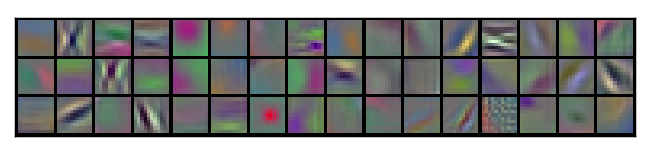
\includegraphics[scale=0.5]{images/good_filters.png} % need to crop to get side by side
	\caption{filters learned in a successfully optimised lowest convolutional layer} 
	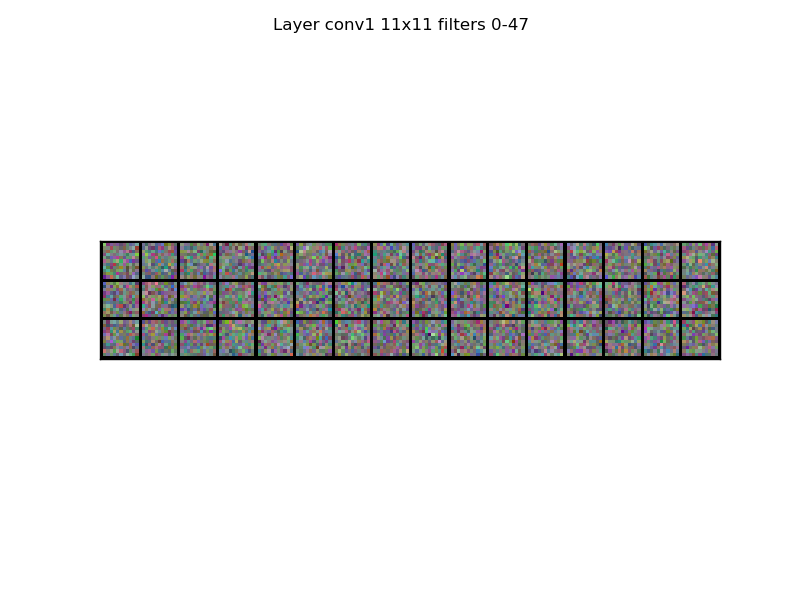
\includegraphics[scale=0.5]{images/bad_filters.png}  % need to crop to get side by side
	\caption{filters learned at lowest convolutional layer of this network}
\end{figure}

This local minimum is `fake' because, with perfect class balance, it would not exist. Or at least, it would correspond to a $\frac{1}{K}$ error rate (where $K$ is the number of classes). One may even call such a minimum `lazy': it would correspond to a human not wanting to make the effort of learning, using instead a strategy of calling out the same label every time without inspecting the image, and still scoring 90\% accuracy in this case. Note that accuracy refers to the percentage of correctly classified cases in the validation set. \\

With this experiment, it becomes clear that class imbalance is a danger not sufficiently when there exists a class that is far more present than another, but sufficiently when there exists a class that takes up a vast majority of the training set. Indeed, the value of the `fake' minimum in terms of error rate is $1 - p_K$, where $p_K$ is the proportion of majority class cases. 

The two situations are only equivalent in the 2-class case; otherwise, the latter is less likely to occur. This may shed light on why class imbalance is not a richly documented issue in the deep learning literature, since benchmark image classification datasets (such as CIFAR, MNIST and ImageNet) involve 10-1000 classes. 

This experiment provides a sufficient condition for class imbalance to be dangerous; necessary and sufficient conditions are discussed in the Experiments section dedicated to class imbalance.

\subsubsection{Mislabelling}

It came as a surprise that, when the same clamp detection task was trained on the tenfold smaller 13,790 Bluebox dataset for which the majority class represents 88\% of images, the model succeeded in learning, as the downward trend in training error and convex trend in validation error show. The achieved performance was 83.9\% validation accuracy.

\begin{figure}[h!]
	\centering
	\begin{subfigure}{.5\textwidth}
  		\centering
		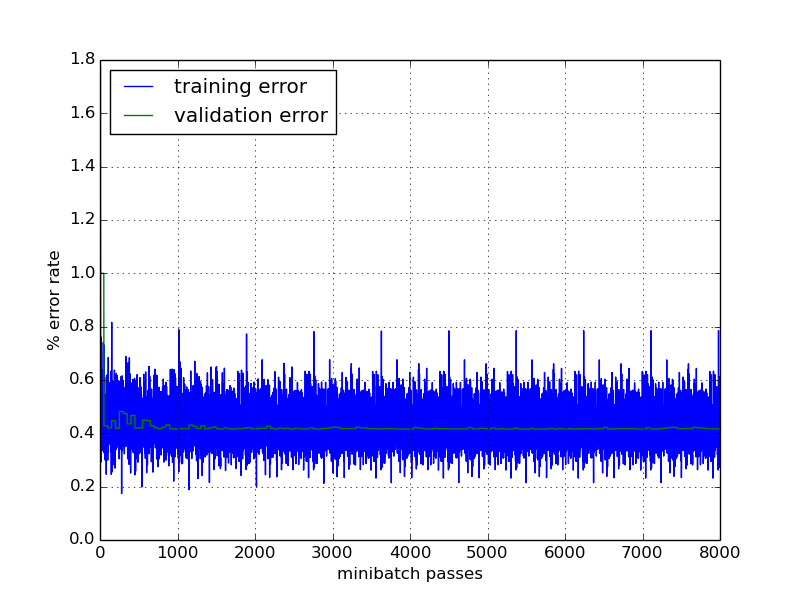
\includegraphics[scale=0.4]{images/increase_test_precision.png}
		\caption{Clamp Detection on Redbox}
	\end{subfigure}%
	\begin{subfigure}{.5\textwidth}
  		\centering
		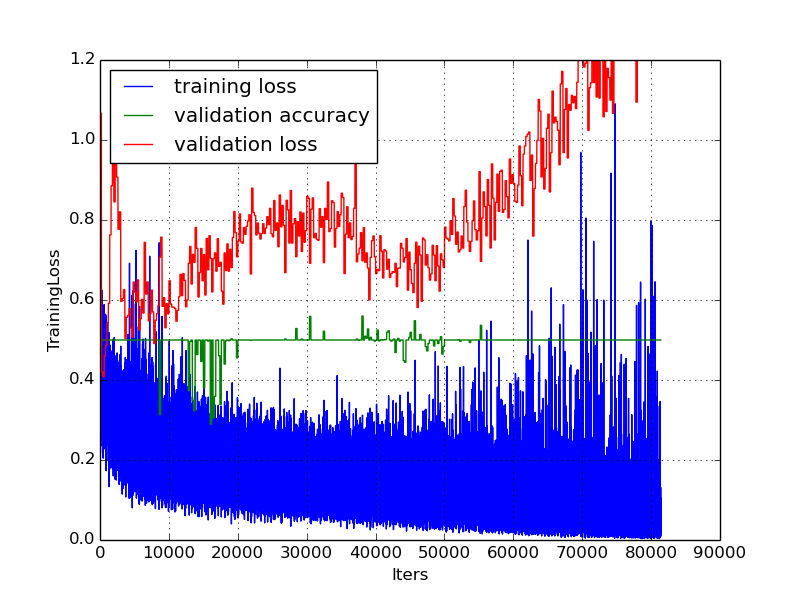
\includegraphics[scale=0.4]{images/plot_clampdet_tl_wout.png}
		\caption{Clamp Detection on Bluebox}
	\end{subfigure}
\end{figure}

A smaller training set is supposed to deliver weaker performance, because it provides the model with less information to learn from, and is more sensitive to overfit. However, after visually inspecting random samples from the Redbox training set, it was discovered that it suffered from heavy mislabelling. For example, out of 50 images randomly sampled from those Redbox images for which no flags were recorded - which are therefore supposed to be images of perfect weld installations - visual inspection performed with the help of a trained ControlPoint employee revealed that 22 of them should have received at least one flag. Three of them are given below.

\begin{figure}[h]       
    \fbox{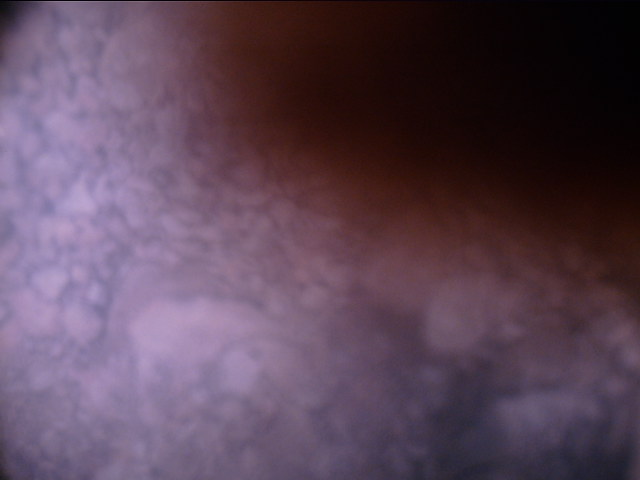
\includegraphics[scale=0.23]{images/66347.jpg}}   
    \hspace{5px}
    \fbox{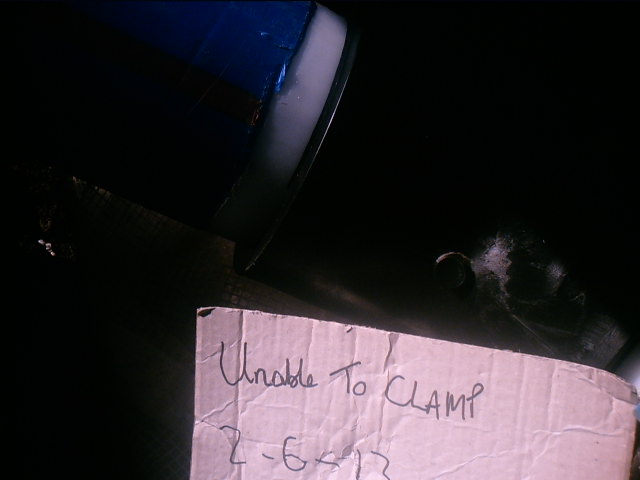
\includegraphics[scale=0.23]{images/104887.jpg}}
    \hspace{5px}
    \fbox{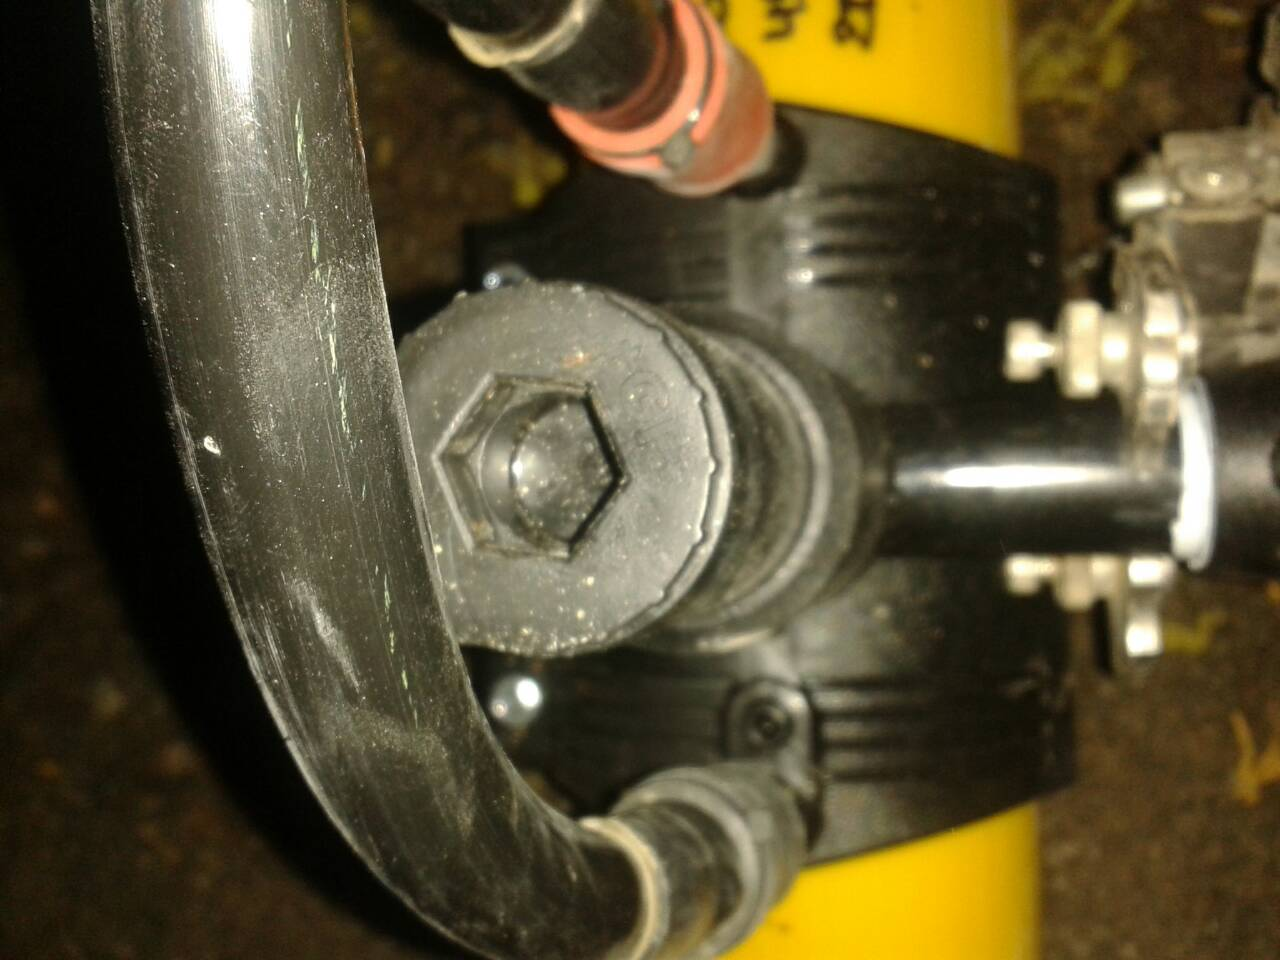
\includegraphics[scale=0.115]{images/100979.jpg}}
    \caption{Redbox images with no flags}
    \label{materialflowChart}
\end{figure}

As can be seen, the image to the left should have received the `Unsuitable Photo' flag (it would have been merged into the `Photo Does Not Show Enough of Clamps' class for training). However, since this one bears no flags, for the clamp detection task it is shown to the network as an example of a weld installation with clamps; for the scrape zone detection task, it is an example of a weld installation with visible scrape zones; etc. The middle case is almost comical: it too is shown to the network as an example of a weld installation with clamps, despite it being \textit{literally} obvious that clamps are not present. Finally, the image to the right is zoomed in too closely for clamps to be visible. 

Discussion elucidated that the beginnings of ControlPoint's pipe weld monitoring services were met with human and technical difficulties which may have resulted in data being misclassified. This would explain why learning is more successful on the Bluebox data: the Bluebox apparatus was shipped to clients later, at a stage when these difficulties had been overcome.

Deep neural networks have been reported to be robust to mislabelled data \cite{DL-book}, but if the proportion of correctly labelled examples is lower than the proportion of majority class examples, then bad minima are not just likely to occur, they are inevitable. Consider a hypothetical classifier with perfect understanding of the classes (e.g.\ a human expert from ControlPoint) which always assigns the true label to any image, and a `lazy' classifier which always assigns the majority class label to any image. Consider also a dataset with majority class proportion $k$ and random assignment of incorrect class labels to a proportion $r$ of that dataset. The perfect classifier will obtain a $1-r$ error rate, whereas the lazy classifier will obtain a $k$ error rate. If $r > 1-k$ then the lazy classifier will beat the perfect classifier. For clamp detection on the Redbox dataset, this is the case if more than $10.8\%$ of images are missing a `No Clamps Used' or a `Photo Does Not Show Enough Of Clamps' flag. 8/50 of the randomly sampled flagless images were failed images akin to the unsuitable image shown above, and 4/50 were of the type shown in the middle or on the right. Since flagless images make up 43\% of the training set, this estimate\footnote{One must concede that the estimate is imprecise due to the small size of the sample.} suggests that approximately $0.43\cdot\frac{8+4}{50} = 10.3\%$ of Redbox images are mislabelled with regards to clamp detection. This would also imply that none of six other, less frequent flags can be learned using the Redbox dataset.

In order to limit the impact of mislabelling, the rest of the project was conducted solely with the use of Bluebox data. This heavily reduced the amount of training data, motivating the use of transfer learning. It is worth noting that there is probably scope for making use of some of the Redbox data by exploring ways of filtering out some of mislabelled data; this is discussed in the conclusions of the report. This path was not chosen because making use of transfer learning seemed to offer more focus on deep learning techniques than on characteristics specific to the datasets.


\clearpage
\section{Experiments 2: Transfer Learning}

\subsection{Motivations}

 These results, combined with the data limitations of restricting ourselves to the Bluebos dataset, motivate the use of transfer learning in this project. This section consists in exploring and understanding the effects of transfer learning on the clamp detection task. Restricting work to the clamp detection task rather than all tasks enabled faster evaluation of alternative approaches to transfer learning, which was crucial given that a single model took 2-30 hours to train. 


\subsection{Implementation}

\subsubsection{Caffe}

Since the open-sourcing of Cuda-Convnet, other deep learning labs have made use of Krizhevsky's CUDA code to develop more modular APIs for GPU implementations and additional features \cite{caffe} \cite{theano} \cite{torch7}. One that is noted for its transfer learning feature is Caffe, an open source framework for convolutional neural network algorithms, developed by Yangqing Jia's team at the Berkeley Vision and Learning Center. It provides the Caffe Reference ImageNet Model, a slightly lesser performing imitation of AlexNet \cite{decaf} that is the 313,000th iteration of training an identical architecture on the 1.3 million image ILSVRC 2012 labelled data. This model achieves 19.6\% top-5 validation error, compared to 18.2\% for (Krizhevsky et al 2012). Caffe also provides an interface and underlying back end for choosing which layers to transfer. In terms of computational efficiency during backpropagation, Caffe is currently the best, requiring 1.787 seconds per mini-batch training iteration for a 128 image mini-batch size and 224x224 images \cite{soumith-benchmark}. Caffe is the only implementation for which backpropagation is written entirely in C++ and CUDA, so this may be why. 

An important note is that the Caffe Reference ImageNet model is licensed for academic research, and is for non-commercial use only. Therefore, if ControlPoint wishes to make commercial use of a network whose weights were initialised from it, it would have to pretrain its own net on a dataset on which there are no such licensing restrictions. \\

It took two weeks to install Caffe, write data batching scripts in Python, understand how to manipulate it and successfully start training. A small contribution to the Caffe open source project was made: symlinking data to the task directory instead of copying it. Previously, copies of the data were made for every task. One could use the same directory for several tasks, but in the context of tackling class imbalance, it is desirable to keep control of class proportions in the training set; flexibility is therefore required to be able to take several different subsets of the training set. As a result, one usually ends up requiring multiple different data directories, hence the benefits of symlinking the data. 


\subsubsection{Per Class Accuracy Layer}

A new per class accuracy layer was written in C++ to replace the accuracy layer used to compute validation error and validation accuracy. It had to be inscribed within the object-oriented framework that Caffe is written in, as well as all of the proto buffers, space restrictions, custom memory and arithmetic operations that were specifically designed and written by the Caffe developers for optimal training of models on a GPU. This required becoming familiar with the design of the entire project. Moving from making modifications to a large scale machine learning framework written fully in C++ was challenging -- particularly after having got used to Cuda-Convnet's Python interface -- and took several weeks. Once written, tested and debugged, the per class accuracy layer was also contributed to the Caffe open source project. 

The layer computes the same softmax cross entropy for the error, but instead of computing the percentage accuracy over the validation set, it computes the average per class accuracy over the validation set. This metric is arguably the real metric of interest for this task: ControlPoint have explicitly stated that there would be no value in using a classifier that is a constant function in the case of detecting a flag that, for example, occurs only 1\% of the time. Such a classifier would score 99\% accuracy but only 50\% average per class accuracy.

Another useful aspect of the average per class accuracy layer is that it serves as a symptom checker for class imbalanced-induced bad minima: indeed, if the model is stuck in such a bad minimum, then it is a constant function; therefore, in the case of a binary classifier, its per class accuracy can only be 50\%, regardless of the class imbalance. However, a limitation of such a layer is that 0.5 per class accuracy could in principle be caused by other factors than a bad minimum - it is in this sense that it can serve as a symptom checker rather than a true detector. This aspect was overlooked at first and lead to misleading conclusions during research which have since been revised. 


\subsection{Experimentation}

Transfer learning for clamp detection consists in taking the Caffe Reference Imagenet model, removing the 1000-output softmax layer (since the model was trained on the 1000 class ILSVRC 2012 challenge), and replacing it with a 2-output softmax layer the with randomly initialised weights. Since the features are encoded by the weights, copying the weights amounts to transferring the learned features.

Note that following visual inspection of the `No Clamps Used' and 'Photo Does Not Show Enough of Clamps` classes, the boundary between the two appeared to be very fuzzy; this was confirmed by the fact that ControlPoint employees themselves tended to disagree on which of the two flags was more suitable for certain images. As a result, the two classes were combined into a `No Clamps' class for the rest of the project. \\

Experimentation consisted in exploring three hyperparameters related to transfer learning: whether to freeze backpropagation on any layers in order to maintain the features of the transferred model, whether to randomly initialise rather than copy the weights of certain layers in order to give these layers `greater freedom' to learn \cite{transfer-learning}, and finally, whether to learn weights by minimising a logistic, therefore parametric loss function, or a hinge loss function, which is non-parametric and amounts to training a Support Vector Machine. 


\subsubsection{Test Run}

As a test run, transfer learning was implemented on a network with the same architecture as was previously used, AlexNet. The training data, as is the case for all subsequent experiments, consists in the Bluebox dataset. Below are the training results alongside those for a model trained identically in all respects apart from weight intialisation, which was fully random. 

\begin{figure}[h!]
	\centering
	\begin{subfigure}{.5\textwidth}
  		\centering
		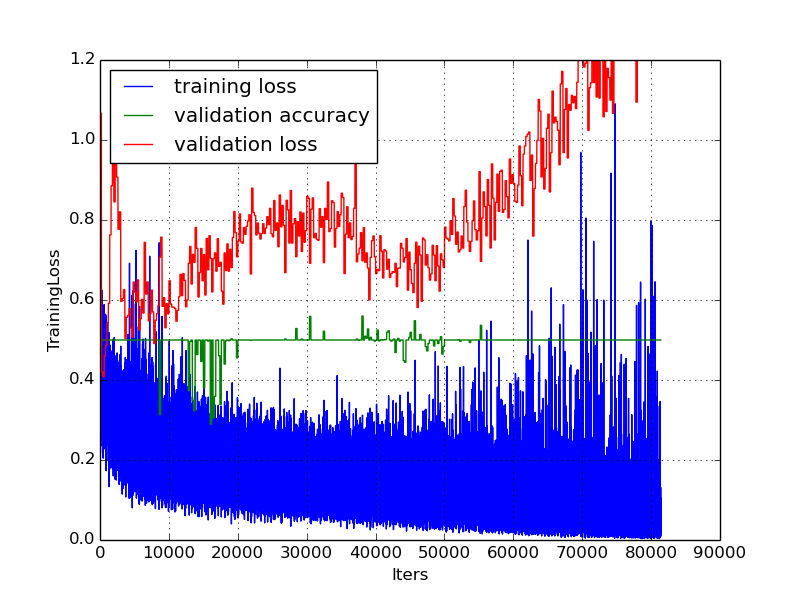
\includegraphics[scale=0.4]{images/plot_clampdet_tl_wout.png}
		\caption{Clamp Detection on Redbox}
	\end{subfigure}%
	\begin{subfigure}{.5\textwidth}
  		\centering
		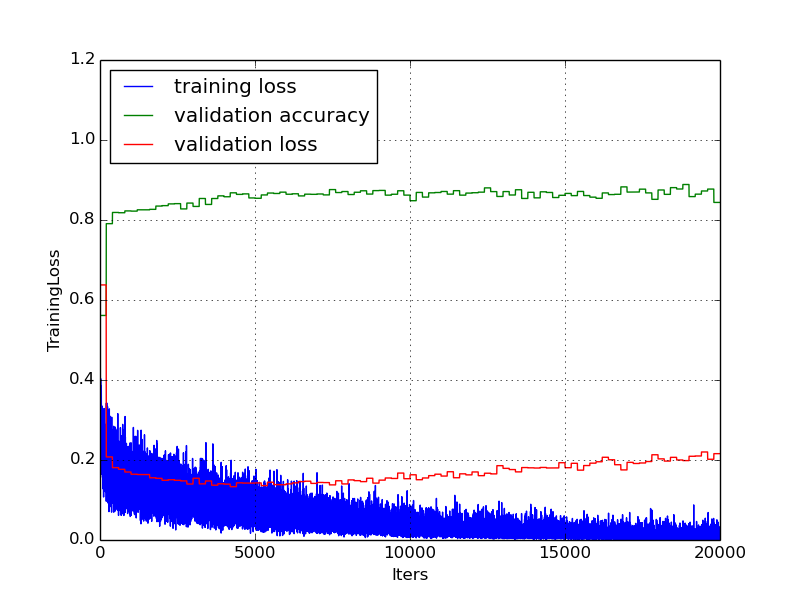
\includegraphics[scale=0.4]{images/plot_clampdet_none.png}
		\caption{Clamp Detection on Bluebox}
	\end{subfigure}
\end{figure}

As can be seen, the model with transfer learning reaches its minimum validation error ten times faster than the model without, and this error is logprob 0.4 lower, which corresponds to pushing average per class validation accuracy up from 83.9\% to 88\%. The gain in convergence comes a significant advantage for coping with the time constraints of the research project. 

\paragraph{Error-accuracy mismatch}

A surprising observation is that the per class accuracy continues to rise long after the validation error reaches its minimum. Maximum accuracy is reached at a point where the model is well into overfit. One wonders what happens to the model throughout this period. One possibility is that the model increases its precision on the minority class at the slight expense of precision on the majority class: this results in a higher per class accuracy, but since the validation error is weighed more heavily by the majority class, it rises. This hypothetical explanation is based on the mismatch between averaging the performance metric across the dataset and averaging across classes. \\

Another possibility is that the model continues to learn features of the data which enable it to correctly classify a slightly higher number of cases, and somehow also lead it to output significantly sparser probabilities (i.e.\ to be highly confident about its predictions) in cases where classification is incorrect. As a result, the number of mistakes decreases, but the euclidean distance between prediction and target within the leftover mistakes increases a lot more. The latter consequence penalises validation error but not percentage accuracy, hence the growth in both. This hypothetical explanation is based on the fact that cross entropy takes a continuous measure of error per case, whereas accuracy takes a binary measure of error per case. \\

Experiments in the next section, on class imbalance, with the softmax Bayesian cross entropy, provided evidence to support the first explanation. The case is then discussed at greater length.

\paragraph{Zig-zag}

Two other noticeable aspects in training without transfer learning are the higher training error amplitude, and the increasing frequency of outlying training error values as training progresses. Both are likely due to the fact that the learning rate is too high; as a result, the network parameters zig zag towards the minimum with greater strides, and the zig zag is accentuated. A graphical illustration of zig-zag where the error surface is simplified to a quadratic bowl is given below. 

\begin{figure}[h!]
	\centering
	\begin{subfigure}{.5\textwidth}
  		\centering
		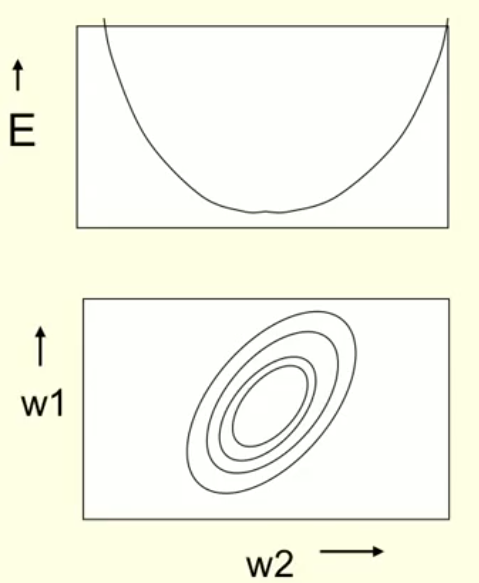
\includegraphics[scale=0.3]{images/gradient_descent_ellipses.png}
		\caption{Vertical and horizontal slices of error surface}
	\end{subfigure}%
	\begin{subfigure}{.5\textwidth}
  		\centering
		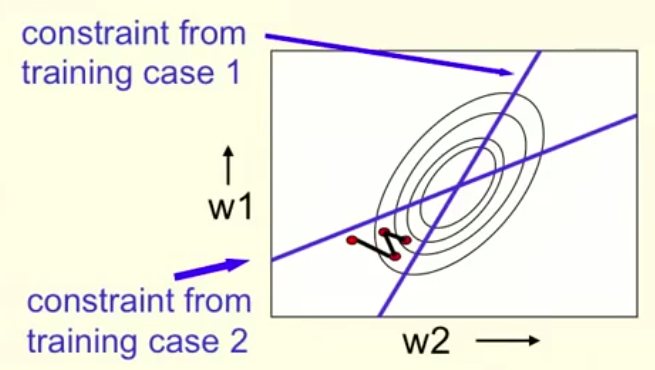
\includegraphics[scale=0.3]{images/gradient_descent_zigzag.png}
		\caption{Steepest descent causes zig zags}
	\end{subfigure}
	\caption{source: Coursera, Neural Networks for Machine Learning}
\end{figure}

If greater zig-zag occurs on the net without transfer learning, one may wonder why. This may come across as contradictory: it can be seen on the graphical illustration that as the parameters come closer to the minimum, smaller steps (i.e.\ learning rate) are required. SGD tricks lecture 6 provides an answer: the bias is optimal with transfer learning, so bowls are rounder.

In light of this explanation, faster convergence for the no transfer learning task could have been obtained by using a smaller learning rate, but the objective of the test run was to train two networks, identical across all aspects save for transfer learning. One conclusion is that transfer learning enables the use of a higher learning rate, which partly explains why convergence is faster. \\

The essential takeaway from the test run is that initialisation of the parameters is very important, even in convolutional neural networks, at least when the dataset is not large as is the case with the Bluebox dataset. This is consistent with previously mentioned findings by (Glorot et al 2013) \cite{rectifier}. \\


\subsubsection{Freezing Backprop on various layers}

An aspect of transfer learning that can be explored is whether to freeze backpropagation on part of the network during training. Since the error-weight partial derivatives are computed using the chain rule, the feed-forward architecture of a network implies that computing them for one layer requires computing those in the layers above. However, one may wish to propagate the gradient back to only a certain layer in the network, in order to hold fixed the features that have been learned in the lower layers. In the case of CNNs, a potential motivation would be to maintain the convolutional filters of the lower layers, which tend to generalise best to any computer vision task \cite{transfer-learning}, and constrain the network to optimise over the training set only with the use of fully connected layers. The intuition here would be that, by enabling full backpropagation, weights would be updated in directions that are optimal for fitting the training data, but that may not generalise well to unseen data. \\

Experiments were run by training 8 models identically in all respects save for the number of layers on which to freeze backpropagation. Training results are not all illustrated below because incremental differences are indistinguishable; instead, the two sides of the spectrum are given: backpropagation enabled on all layers (i.e.\ the test run transfer learning model) and backpropagation enabled only on the randomly initialised softmax output layer. 

\begin{figure}
    \centering
    \begin{minipage}[b]{\textwidth}
      \begin{subfigure}{.5\textwidth} 
        \centering
        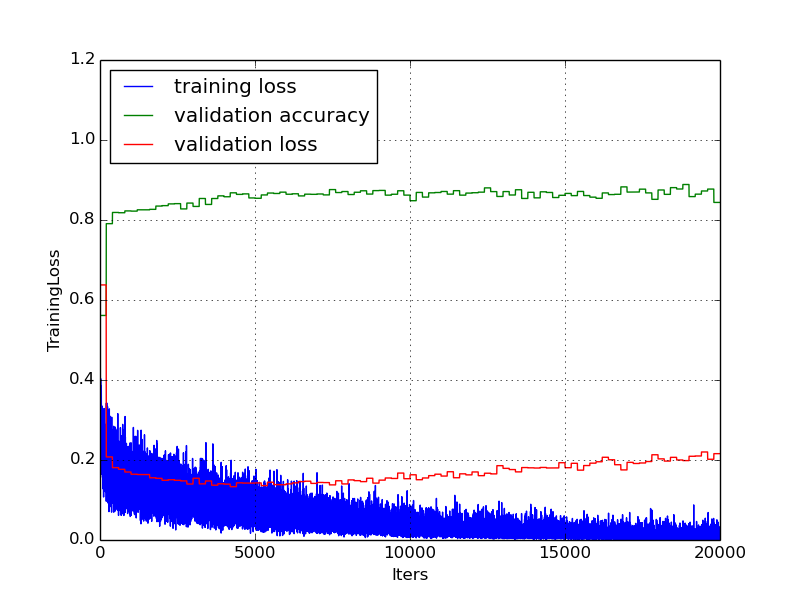
\includegraphics[scale=0.4]{images/plot_clampdet_none.png}
        % Add \par\vspace*{20pt} here and...
        \caption{backprop on all layers}\label{fig:2a}
      \end{subfigure}%
      \begin{subfigure}{.5\textwidth} 
        \centering
        \includegraphics[scale=0.4]{images/plot_clampdet_fc7.png}
        % ...here to lower the subcaptions and...
        \caption{backprop on top layer only}\label{fig:2b}
      \end{subfigure} \par \vspace*{20pt} % ...remove them from here
    \end{minipage}%
\end{figure}

The main difference is in the training error: when backpropagation is restricted to a single layer, the model is unable to perfectly fit the data. This is simply a result of having constrained the expressiveness of the model, much like trying to fit a curve with a lower-order polynomial. However, the advantage is that the model does not overfit. Between the two extreme cases, full backpropagation achieves 88\% average per class validation accuracy at best, whereas minimal backpropagation achieves 85.1\%. 

However, there is an optimal middle ground: freezing backpropagation on four of the five convolutional layers achieves a maximal average per class validation accuracy of 89.2\%. A potential explanation for this is the one given above, namely that freezing backpropagation on lower layers conserves optimal features, forces the model to make more effort to fit the data with the limited use of the upper layers, and generalises better. \\


\subsubsection{Initialising Free Layers}

Another hyperparameter is whether to re-initialise the layers in which backpropagation has been enabled to the transferred network's weights, or to randomly initialise them. A way to think about this intuitively is to wonder: do we want to keep the features learned at the given layer or not? 

The features on convolutional layers are easy to visualise, and the success of transfer learning in computer vision rests on the fact that pixel features good for one computer vision task are also good for others. This makes intuitive sense for low level shapes: our visual world is made up of combinations of edges, corners, textures and shapes. But what about the features in the fully connected layers? There currently exists no way of visualising the semantic content in fully connected layers, so it is not obvious whether or not the features in the fully connected layers are of any use for transfer tasks. This motivates experimentation with weight re-initialisation. 

A further motivation is existing empirical research \cite{transfer-learning} \cite{decaf} on transfer learning which finds that re-initialising weights gives the layers `more freedom' to learn. In light of Yann LeCun's recent comments regarding the training of CNNs\cite{labex-bezout}, one could visualise this as initialising the weights inside or outside the `narrow band' where the minima are `clustered'. It would be harder to navigate inside a region that were densely filled with extrema that are optimal for the source task but not the target task.  \\

\begin{figure}
    \centering
    \begin{minipage}[b]{\textwidth}
      \begin{subfigure}{.5\textwidth} 
        \centering
        \includegraphics[scale=0.4]{images/plot_clampdet_none_reinit.png}
        % Add \par\vspace*{20pt} here and...
        \caption{Random initialisation of fully connected layers}\label{fig:2a}
      \end{subfigure}%
      \begin{subfigure}{.5\textwidth} 
        \centering
        \includegraphics[scale=0.4]{images/plot_clampdet_none-10k.png}
        % ...here to lower the subcaptions and...
        \caption{Full transfer of weights}\label{fig:2b}
      \end{subfigure} \par \vspace*{20pt} % ...remove them from here
    \end{minipage}%
\end{figure}

One observes that with randomly re-initialisation of weights, the training error starts higher. This is understandable and could be explained by the fact that the network starts in an area of the parameter space which is further away from the `minima cluster band'. Secondly, the training error is more volatile: this is a result of the network having `more space to move'. As a result, overfit occurs sooner too. 

Re-initialising the weights barely increases performance when measured by average per class accuracy: 86.4\%, versus 86.1\%. does not increase performance overall:  average per class accuracy is obtained, versus since is not in line with other experimental results \cite{transfer-learning}. Perhaps, if data had been more plentiful, re-initialisation would have proven superior. However, given that the backpropagation is fully enabled in such a network that is very large relative to the dataset (remember this network size was trained on ImageNet), overfit occurs quickly.


\subsubsection{Softmax vs linear SVM}

`CNN features off the shelf' by Razavian et al, 2014, \cite{off-the-shelf} established state-of-the-art results by training linear SVMs on the features from the 7th, fully connected layer of OverFeat. One may wonder why Razavian et al train a linear SVM rather than a conventional softmax layer, and whether the difference in performance is substantial. A second motivation for this comparison is to reproducing the technique of (Razavian et al 2014)\footnote{with the exception that the transfer model used here is not OverFeat, but the slightly lesser performing Caffe Reference ImageNet model.} to provide a benchmark for the optimisations and results produced by this research project\footnote{The benchmark would have been better carried out by using OverFeat, but the model is only available for Torch7, an alternative framework to Caffe.}.

\paragraph{Analytical Comparison}
The difference between the two can be fully expressed as a difference between cost functions\cite{ML-book}: hinge loss and cross entropy loss. What follows is a numerical comparison of the two \footnote{Heavily drawn from (Bishop 2010)}. 

(Razavian et al 2014) implement transfer learning by freezing backpropagation on all transferred layers, replacing the softmax output layer with an inner product layer containing as many output units, and training by minimising a hinge loss. Indeed, the SVM optimisation problem exposed in the literature review can be reformulated as the minimisation of the $L_2$ regularised hinge loss cost function \cite{ML-book}, given by:

\begin{equation}
\mathcal{C}_{hinge}(\textbf{w}, b) = \frac{1}{n}\sum \limits_{i=1}^{n} max(0, 1 - t_i(\textbf{w}^T \phi(\textbf{x}) + b))
\end{equation}

Note that the cost function is denoted as a function of the weights and bias, since these are the parameters that are allowed to vary in order to minimise the expression. The formula can understood by bearing in mind that with binary SVMs, target label values are \{1, -1\}. Therefore, when the prediction is perfect, $t_i(\textbf{w}^T \phi(\textbf{x}) + b) = 1$.\\

On the other hand, a softmax output layer with two output units performs a logistic regression \cite{ML-book}:

\begin{equation}
\psi(\textbf{x}) = \frac{1}{1+\exp(\textbf{w}^T \phi(\textbf{x}) + b)}
\end{equation}

Since logistic regression has range [0, 1] but linear SVM has range [-1, 1], we need to rescale logistic regression output values for the ranges to match, in order to define the hinge and softmax cost functions over the same domain. This can be done by taking $\psi_{rescaled}(\textbf{x}) = t_i \psi(\textbf{x}_i)$. The maximum likelihood estimates of the parameters with logistic regression are obtained by minimising the negative of the log-likelihood function over the training set; this is colloquially referred to as the logprob and can be proved to be the cross entropy. When reformulated with SVM target labels it is given by: 

\begin{equation}
\mathcal{C}_{CE}(\textbf{w}, b) = \frac{1}{n} \sum\limits_{i=1}^{n}\log(1 + \exp(-t_i(\textbf{w}^T \phi(\textbf{x}) + b)))
\end{equation}

In order to compare the two cost functions, we first needed the definition domains to match. Since a cost function takes a model's output as input, this meant ensuring that the output domains of a softmax layer and a linear SVM match; hence the rescaling of the logistic regression output values. However, we also need to rescale the \textit{output} values of one of the cost functions so as to make both cost functions have the same output for a specific input value, and then see how the two compare for the rest of the definition domain. The reason for this is that a model's parameters are trained by minimising a cost function, so the value of this minimum is irrelevant. Just because one cost function's minimum value is 0 and another's is 10 does not mean that the latter model performs worse than the former. In order to see whether cost function A punishes a certain type i of error more heavily than function B does, one must see whether punishment for type i error compared to punishment for type ii error is different with cost function A than with cost function B. Numerically, this can be done by rescaling the output of a cost function for it to equal the output of the other cost function at a specific point, and then see how the outputs for the two cost functions differ along the rest of the definition domain.

In this case, by rescaling the softmax error by $\frac{1}{\log(2)}$, we get equal output for input value 0. A graphical representation can be seen below. \\

\begin{figure}[h!]
	\centering
	\includegraphics[scale=0.3]{images/hinge_vs_ce.png}
	\caption{Hinge (blue), cross entropy (red), mean squared error (green). source: (Bishop 2010)}
\end{figure}

With target labels \{-1, 1\}, 0 corresponds to total classification uncertainty (i.e.\ input is considered as likely to belong to one class as the other). For $z \in (0,1]$ (i.e.\ correct classification), the softmax loss is above the hinge loss, and for $z \in [-1,0)$ (i.e.\ incorrect classification), the softmax loss is under the hinge loss. In intuitive (and slightly abusive) terms, this means that the hinge loss continues to penalise even when the classification is in the correct region, but is more lenient when the classification is in the incorrect region. In colloquial terms, this is like saying `make highly confident predictions, even if that means sometimes making mistakes'. The bottom line is that this encourages sparser output probabilities.

\paragraph{Empirical Results}

The linear SVM was implemented in Caffe by designing an 8-layer model, with the 7 bottom layers transferred from the Caffe Reference Imagenet model, the top layer an inner product layer with element-wise product activation functions: in other words, no non-linear activation, just the linear operation $\textbf{w}^T \textbf{x} + b = 0$, where \textbf{x} is the output of the 7th layer. Finally, the model is equipped with a hinge-loss layer. Note that it was not equipped with a hinge loss (validation) accuracy layer, but was rather given the standard per class accuracy layer, which outputs the softmax cross entropy as validation error. \\

\begin{figure}
    \centering
    \begin{minipage}[b]{\textwidth}
      \begin{subfigure}{.5\textwidth} 
        \centering
        \includegraphics[scale=0.4]{images/plot_clampdet_none.png}
        % Add \par\vspace*{20pt} here and...
        \caption{log prob cross entropy loss}\label{fig:2a}
      \end{subfigure}%
      \begin{subfigure}{.5\textwidth} 
        \centering
        \includegraphics[scale=0.4]{images/plot_clampdet_linSVM.png}
        % ...here to lower the subcaptions and...
        \caption{hinge loss}\label{fig:2b}
      \end{subfigure} \par \vspace*{20pt} % ...remove them from here
      \caption{hinge loss}\label{fig:2}
    \end{minipage}%
\end{figure}

We observe that the training error does not converge to zero with the hinge loss, which means that the training data projected on fc7 space is not linearly separable. This does not come as a surprise and confirms the complexity of the clamp detection task. As discussed in the numerical analysis, the errors between these two models are not comparable since they are of different nature. Just because the hinge loss is higher in absolute terms than the cross entropy does not mean that test run performance is lower. 

The way to compare performance in the two models is to look at average per class validation accuracy: 85.4\% for linear SVM versus 85.1\% for softmax. The difference is only very slight, but is consistent with the choice of Razavian et al to train a linear SVM, as well as other recent empirical results \cite{svm-nn}. This also casts in good light the optimisation achieved by freezing backpropagation on the first four convolutional layers, since by achieveing 89.2\% it beats the technique adopted by (Razavian et al 2014) by nearly 4 percentage points.


\clearpage
\section{Experiments 3: Class Imbalance}

\subsection{Definition}

Before detailing the motivations for the experiments that took place, we properly return to the definition of class imbalance mentioned in the literature review and during the discussion of results on simple clamp detection. An extension to this definition is proposed to encompass \textit{dangerous} class imbalance. Having such a definition provides a framework for reasoning about the problem.

Class imbalance has been defined as the situation where the sample distribution of classes is significantly non-uniform. For example, (Pastor-Pellicer et al 2013) \cite{f-measure} define it as when `the number of patterns of one class is significantly lower than other classes'. However, consider a 12-class training set where 11 classes each take up 9\% of the dataset and the 12-th takes up 1\%. Outputting the same class all the time cannot provide more than 9\% accuracy, which is only slightly better than `completely random guessing', which would achieve 8.3\% accuracy\footnote{To the best of our knowledge, in this case there is no classification strategy that would score higher than 9\% without making use of information contained in the input. It would be preferable to prove it, but due to time constraints, this has been left for further research.}. \\

Class imbalance is defined in this report by the situation where \textbf{a classifier that constantly outputs the class priors performs significantly better than randomly outputting each class with the same probability}. To better understand this definition, one can take note of the property that outputting the prior classifies all input into the majority class. What follows are examples that justify this non-trivial definition.

\begin{enumerate}
\item Given a 2-class dataset with distribution of classes (0.9,0.1), a classifier which outputs (0.9,0.1) all the time will classify all cases into the majority class, and obtain 90\% accuracy. On the other hand, randomly outputting them uniformly obtains only 50\%. 
\item It is not necessary for a class to occupy the vast majority of the training set: consider a 1000-class training set where one class takes up 20\%. A classifier which outputs the prior all the time will obtain 20\% top-1 accuracy, compared to 0.1\% for random uniform. 
\item It is not necessary for a class to occupy far more space than any other. Consider a 1000-class training set where 5 classes each take up 17\%. Outputting the prior all the time obtains 85\% top-5 accuracy, which for example is higher than the score of (Krizhevsky et al 2012) at ILSVRC 2012 \cite{krizhevsky}.
\end{enumerate} 

It would be tempting to make the conjecture that outputting class priors is the best performing constant function classifier not just with respect to percentage accuracy, but also Maximum Likelihood Estimation (i.e.\ cross entropy when using a softmax layer) and Mean Square Error. However, due to time constraints there was insufficient time to attempt to prove this; it is left for further research. \\

With a clear definition in mind, we now return to motivations for the class imbalance related experiments that were carried out. \\

\subsection{Motivations}

The first challenge posed by the Bluebox dataset was its small size, the second was class imbalance. Although transfer learning by itself delivered strong results for clamp detection and other tasks, models failed to learn (in the sense that average per class accuracy remained at 0.5) for 9 tasks on which class imbalance was more pronounced. \\

Therefore, additional approaches for dealing with class imbalance were sought out. However, instead of trying them out on the unsatisfactory tasks, they were tried on a subset of the clamp detection dataset where class imbalance was increased (simply by throwing out training cases without clamps). This way, one knows that the only thing preventing performance on the task is class imbalance, and the impact of an approach on classification performance is a good measure of the impact of the approach on class imbalance. \\

Were this tactic not adopted, it would not be possible to ascertain whether an approach failing to deliver a performance increase were due to its inability to tackle class imbalance, or to the fact that the task is difficult  for other reasons. For example, water contamination risk is defined by the presence of droplets on the pipe fitting. However, when images are downsized to 256x256 pixels for AlexNet, droplets become invisible to the naked eye. This task could therefore be impossible to learn with networks the size of AlexNet, for a reason not related to the strong class imbalance that the task also presents (92.5\%). \\




\subsection{Implementation}

Several class imbalance-tackling techniques that were experimented with required development. A Python program was written to under-sample or over-sample from a class. Two new Caffe layers were written in C++: a `Bayesian softmax loss layer' for training a CNN on a novel cost function and a `Bayesian per class accuracy' layer for computing validation error with the same cost function. Specific motivations and formulae for each are detailed in the experimentation subsection of this section. Following their success in this project's experiments, they were contributed to the Caffe open source project.

%increase class imbalance:
%$target = (max_num) / (total_num - delete_min)
%target*total_num - target*delete_min = max_num
%target*delete_min = target*total_num - max_num
%delete_min = total_num - (max_num/target)$

%\subsubsection{Class Imbalance Solver}
%
%Note that class imbalance ratio i.e.\ size of largest class relative to smallest class is not the right metric to consider. The right metric to consider is the proportion of the largest class, since this is what provides a bad/fake local minimum. This may not seem to be significant but it can be. Consider the 3 class case where we have 10, 100, 500 images for each respective class. Class imbalance ratio is 0.05, and proportion of largest class is approximately 0.82. If we wanted to attain a class imbalance ratio of 0.2, no class would be permitted to have more than 5*10=50 images, and we would be left with a training set of size 110. On the other hand, if we wanted to attain a proportion of largest class of 0.8, we would merely have to remove 12 images from the largest class, and we would be left with a training set of size 598. Interestingly, in the two class case, optimising with respect to either of the two metrics is equivalent. \\
%
%Ok, but do we care about this for this project? Are we ever going to be training multi-class classifiers? Yes, if we think that it may help training to distinguish multiple cases. Intuitively, if two classes contain similar semantic content (e.g. inadequate clamp fitting and no clamp detected both involve clamps), then it could be better to train a single classifier on a 3-class task rather than 2 binary classifiers, because in the latter case, we lose potentially useful information that the images contain about clamps. In other words, to detect whether clamps are fitted properly, it helps to know what a clamp looks like, i.e.\ it helps to know which images do and don't have clamps. \\
%
%t: target bad min
%N: total number of current images
%n: number of majority class images
%k: number of majority class images to kill
%
%when n-k is optimal, we have t = (n-k)/(N-k)
%<=> t*N - t*k = n - k
%<=> (1-t)*k = n - t*N
%<=> k = (n-t*N)/(1-t) \\
%
%so solution is to randomly delete $n - n^{*}$ images from the majority class. \\

\subsection{Experimentation}

This section begins with a test run, intended to serve as a benchmark against which to subsequently evaluate six different approaches to tackling class imbalance. The first approach discussed below is transfer learning, so as to form a transition from the previous set of experiments. The second is the simplest, because it merely consists in tuning model hyperparameters. The three that follow are those explored by (Zhou and Liu 2005) \cite{zhou} to specifically tackle class imbalance. The sixth is a novel cost function. A final subsection branches off from an observation concerning training results for this cost function, providing a credible explanation to the error-accuracy mismatch mentioned in the test run of the previous set of experiments. \\

The amount of additional class imbalance to impose on the clamp detection task was chosen in order to trap the model in a bad, sampling-induced local minimum on the Bluebox dataset. This brought the imbalance ratio from 88\% to 98\%, and corresponds to going from 1,323 minority class training cases to 193. \\

\subsubsection{Test Run}

To evaluate the difficulty of the clamp detection task with increased class imbalance, a model was trained from scratch without transfer learning, to be benchmarked with when it was trained on the entire dataset. 

\begin{figure}
    \centering
    \begin{minipage}[b]{\textwidth}
      \begin{subfigure}{.5\textwidth} 
        \centering
        \includegraphics[scale=0.4]{images/plot_clampdet_tl_wout.png}
        % Add \par\vspace*{20pt} here and...
        \caption{88\% class imbalance}\label{fig:2a}
      \end{subfigure}%
      \begin{subfigure}{.5\textwidth} 
        \centering
        \includegraphics[scale=0.4]{images/plot_clampdetCI98_tl_wout.png}
        % ...here to lower the subcaptions and...
        \caption{98\% class imbalance}\label{fig:2b}
      \end{subfigure} \par \vspace*{20pt} % ...remove them from here
      \caption{no transfer learning}\label{fig:2}
    \end{minipage}%
\end{figure}

Whereas with 88\% imbalance it is possible to learn without transfer learning, with 98\% imbalance it is not. The model converges within one iteration to a constant function\footnote{Note that the reason for why the validation error seems to take 200 iterations to suddenly drop is because the validation frequency was set to a large interval of 200 training mini-batch passes, in order to speed up training.} and remains there. \\

Note that for lower levels of class imbalance, the model is able to escape the sample-induced bad minimum. The plot below shows that with 90\% class imbalance for example, the model becomes a constant function at first, and eventually is able to `creep out' of the sample-induced minimum. \\

\begin{figure}[h!]
	\centering
	\includegraphics[scale=0.5]{images/plot_clampdetCI_none.png}
	\caption{Clamp Detection, Full Backpropagation}
\end{figure}

This provides clues about the shape of the error surface in the neighbourhood of this bad minimum, and how varying the level of class imbalance affects it. It suggests that the bad minimum could in fact be a saddle point: a number of weights are at local optimality i.e.\ error-weight partial derivatives are zero, but not all; there is still room for improvement for some of them i.e.\ the error surface remains locally monotonous along some dimensions. This slowly but eventually moves the network away from the saddle point. Training deep neural networks along saddle points is known to exhibit this type of behaviour: training is slowed down but not stopped\cite{DL-book}.

One would be tempted to conjecture that the steepness of the error surface along these dimensions decreases with the extent of class imbalance, and approaches 0 as class imbalance approaches 100\%. This would explain why at some point class imbalance is too high for the model to escape. 

Further analysis and experimentation, especially by seeing whether individual weights in the softmax layer do indeed cease to update, would perhaps make for interesting further work. In the meantime, in order to maintain generality, these points on the error surface will now be referred to as sampling-induced critical points, or simply bad critical points. \\

A final observation to explain is that although the validation error improves smoothly, the validation per class accuracy improves in sudden increments, i.e.\ discontinuously. This is likely a direct consequence of class imbalance in the validation set. Indeed, a weight adjustment that brings the predicted probability of a single minority class case in the validation set from below 0.5 to above 0.5 will decrease the validation error by $\frac{1}{n}$ and increase the validation per class accuracy by $\frac{1}{2n_{min}}$, where $n$ is the validation set size and $n_{min}$ is the number of minority class cases in the validation set. For sufficiently large $n$ and sufficiently high class imbalance, the error change will be infinitesimal but the accuracy change will be discrete.


\subsubsection{Transfer Learning}

\begin{figure}
    \centering
    \begin{minipage}[b]{\textwidth}
      \begin{subfigure}{.5\textwidth} 
        \centering
        \includegraphics[scale=0.4]{images/plot_clampdetCI98_tl_wout.png}
        % Add \par\vspace*{20pt} here and...
        \caption{no transfer}\label{fig:2a}
      \end{subfigure}%
      \begin{subfigure}{.5\textwidth} 
        \centering
        \includegraphics[scale=0.4]{images/plot_clampdetCI98_none_reinit_bs128_lr4.png}
        % ...here to lower the subcaptions and...
        \caption{convolutional layer transfer}\label{fig:2b}
      \end{subfigure} \par \vspace*{3pt} % ...remove them from here
      \begin{subfigure}{.5\textwidth} 
        \centering
        \includegraphics[scale=0.4]{images/plot_clampdetCI98_none_bs128_lr4.png}
        % ...here to lower the subcaptions and...
        \caption{full net transfer}\label{fig:2b}
      \end{subfigure} \par \vspace*{3pt} % ...remove them from here
      \caption{98\% imbalance, varying levels of transfer learning}\label{fig:2}
    \end{minipage}%
\end{figure}

Transfer learning keeps the net's parameters from bad critical points, so the model is not a constant function. Notice this enables it to perfectly fit the training set. However, little is learned that generalises: maximum validation accuracy is 60.1\%. Transferring the fully connected layer weights helps bring this up to 65.4\%. \\

Note that validation error is very low because it is not a per class average: the transfer learning models quickly obtain high precision on the majority class, but struggle to learn the minority one. 

What is arguably a crucial question is whether the difficulty in learning the minority class is the inevitable consequence of having few training examples to learn from, or whether the imbalance ratio is preventing generalising features of the minority class from being learned. If the former, there is no use in searching for ways to tackle class imbalance without throwing away majority class data.  \\

Following the evaluation of transfer learning, a fixed architecture and training strategy were kept throughout the experiments below: backpropagation on all layers, all weights transferred. Although freezing backpropagation on the first four convolutional layers was found to perform best during experiments of the previous section, full backpropagation was adopted in this section for the sake of clarity. The objective of this section is not to achieve the highest absolute accuracy, but rather to compare relative successes of different approaches to tackling class imbalance.


\subsubsection{Hyperparameter Optimisation}

%Notice what happens when validation batch size too small:
%
%\begin{figure}[h!]
%	\centering
%	\includegraphics[scale=0.5]{images/plot_clampdetCI_none_testrun.png}
%	\caption{Clamp Detection, Full Backpropagation}
%\end{figure}
%
%(training files for above now in clampdetCI/BULLSHIT)
%
%Class imbalance is so high that it is sometimes not present in the subset of the validation set that is being tested. In that case, if the model is in bad min, its per class accuracy will be equal to its accuracy on the majority class. We obtain the confusing output above. (Still got to do some maths to prove that assigning majrity class randomly with probability p (not 0.5) will lead to per class accuracy being 0.5 or p depending on whether minority class present). Hence this confusing output, which could wrongly be interpreted as the network steadily learning but sometimes getting stuck in bad min (and getting back out thanks to momentum). \\


%\begin{figure}[h!]
%	\centering
%	\includegraphics[width=0.8	extwidth,natwidth=610,natheight=642]{images/plot_clampdetCI_testrun_higherbatchsize.png}
%	\caption{Clamp Detection, Full Backpropagation}
%\end{figure}

\paragraph{Mini-batch Size}

Since class imbalance reduces the number of minority class cases, it could arguable make information relating to minority class misclassification contained in the gradient more noisy. If so, increasing the mini-batch size should improve performance.

\begin{figure}
    \centering
    \begin{minipage}[b]{\textwidth}
      \begin{subfigure}{.5\textwidth} 
        \centering
        \includegraphics[scale=0.4]{images/plot_clampdetCI98_none_bs128_lr4.png}
        % Add \par\vspace*{20pt} here and...
        \caption{mini-batch size 128}\label{fig:2a}
      \end{subfigure}%
      \begin{subfigure}{.5\textwidth} 
        \centering
        \includegraphics[scale=0.4]{images/plot_clampdetCI98_none_bs256_lr4.png}
        % ...here to lower the subcaptions and...
        \caption{mini-batch size 256}\label{fig:2b}
      \end{subfigure} \par \vspace*{20pt} % ...remove them from here
      \caption{98\% imbalance, different mini-batch sizes}\label{fig:2}
    \end{minipage}%
\end{figure}

These results are surprising: they seem to suggest that increasing mini-batch size decreases performance. Since increasing mini-batch size only reduces noise in the gradient, this would attribute performance increase to greater noise in the gradient. 

However, one notices that from the 1000th iteration onwards, in the 128 mini-batch size network, the time series of the per class validation accuracy (and if one looks closely, of the validation error too) is not convex. In fact, it appears to be random. The fact that per class validation accuracy will increase discontinuously for a single additional correct minority class classification in the validation set supports this claim. Indeed, random weight changes are bound to lead to small increases and decreases in the number of correct minority class classifications. The plot shows indeed as many increases as decreases. These seem substantial but this is only the result of per class accuracy being heavily weighted by minority class cases. If improvements are indeed random, they will not generalise to the test set. \\

A foolproof verification of this explanation would be to run both models on a test set, and see whether there is indeed no significant difference in true performance between the two models. \\	


\paragraph{Learning Rate}

Decreasing the learning rate helps if it prevents a good minimum from being overshot. 

\begin{figure}[h!]
    \centering
    \begin{minipage}[b]{\textwidth}
      \begin{subfigure}{.5\textwidth} 
        \centering
        \includegraphics[scale=0.4]{images/plot_clampdetCI98_none_bs256_lr4.png}
        % Add \par\vspace*{20pt} here and...
        \caption{learning rate 0.0001}\label{fig:2a}
      \end{subfigure}%
      \begin{subfigure}{.5\textwidth} 
        \centering
        \includegraphics[scale=0.4]{images/plot_clampdetCI98_none_bs256_lr5.png}
        % ...here to lower the subcaptions and...
        \caption{learning rate 0.00001}\label{fig:2b}
      \end{subfigure} \par \vspace*{20pt} % ...remove them from here
      \caption{98\% imbalance, different learning rates}\label{fig:2}
    \end{minipage}%
\end{figure}

With a lower learning rate, the validation accuracy seems to increase at a far slower pace. This suggests that there was no overshooting when using the original learning rate value, and that 0.0001 is a good learning rate for this task. \\


\subsubsection{Over-Sampling}

Over-sampling \cite{zhou} \cite{maloof} rebalances the training set to desired levels of imbalance by increasing the occurrence of minority class examples. This was implemented by creating duplicates in the training set -- but not in the validation or test sets, as this would have slowed down the algorithms and biased any performance metric not averaged across classes. Moreover, in order to compare the performance of models trained with different techniques, the same validation set needs to be the same for all models.

\begin{figure}[!]
    \centering
    \begin{minipage}[b]{\textwidth}
      \begin{subfigure}{.5\textwidth} 
        \centering
        \includegraphics[scale=0.4]{images/plot_clampdetCI98_none_bs128_lr4.png}
        % Add \par\vspace*{20pt} here and...
        \caption{98\% imbalance, full backprop, full transfer}\label{fig:2a}
      \end{subfigure}%
      \begin{subfigure}{.5\textwidth} 
        \centering
        %\includegraphics[scale=0.4]{images/plot_clampdetCI98_os_none_bs128_lr4.png}
        % ...here to lower the subcaptions and...
        \caption{Same with over-sampling to 88\% imbalance}\label{fig:2b}
      \end{subfigure} \par \vspace*{20pt} % ...remove them from here
    \end{minipage}%
\end{figure}


Oversampling completely fails. \\

Observations:
- very weak performance
- per class accuracy goes below 0.5
- entire error time series are shifted up by a constant
- overfit occurs sooner


Interpretations:
How can per class accuracy be below 0.5? that's worse than random! It may be due to the fact that copies are made in the training set, but not in the test and validation sets. 
When comparing these networks, should we not be using the same validation set for all? No, we should be using the same test set (and testing will come in the next section). We should choose the validation set that we deem best for early stopping. In the case of over-sampling, makes no sense to include duplicates. 


\subsubsection{Under-Sampling}

Under-sampling rebalances the training set to desired levels of imbalance by removing majority class examples. The brute force approach, implemented in (Maloof 2003) \cite{maloof}, consists in randomly removing these cases and train on the remaining set. However, (Zhou and Liu 2005) \cite{zhou} describe an algorithm for removing selectively. It was not implemented during this project mainly due to its time complexity, which is analysed below. 

\paragraph{Under-Sampling algorithm}
\begin{enumerate}
\item Choose desired imbalance ratios for each non-minority class.
\item Reach desired imbalance levels in training set by randomly setting aside non-minority class examples.
\item Train a net.
\item While there remains examples set aside:
	\begin{enumerate}
	\item Increase training set by bringing in 50\% additional non minority class examples.
	\item Don't train yet, but classify all new arrivals. Remove those correctly classified.
	\item If training set remains unbalanced, remove non minority class examples whose nearest neighbour in feature space is of a different class.
	\item If training set remains unbalanced, randomly remove non minority class examples.
	\item Train the net on the training set.
	\end{enumerate}
\end{enumerate} 

Notice that the removal of majority class examples is selective based first on a `redundant' criterion, then on a `potentially noisy' criterion. The underlying assumption for the first criterion is that examples which are already classified will not contribute to learning. However, if `redundant' is taken formally as stating that back-propagating the gradient from these examples will not modify the weights, then it assumes that the error on them is zero, i.e.\ that the output probabilities for these examples are binary vectors. This is highly unlikely to be the case in practice, so the classification test for rejection does not identify truly redundant examples. 

The second criterion assumes that if an example's nearest neighbour is of a different class, then it is better for learning to discard this `boundary example' because it is likely to be highly noisy. The impact of this selection criterion on learning is based on euclidean distance, it is therefore non-parametric and is difficult to intuit in the context of deep neural networks with softmax output, which are parametric models. On the other hand, the criterion can be intuited in the context of SVM learning. If we were training a Support Vector Machine, i.e.\ finding the decision boundary that leaves most gap between support vectors of different classes, then discarding non-minority class `boundary examples' would have two effects: extend the minority class `territory' into the `territory' of non minority classes, and reduce the error on fitting linear boundaries to the training data. The implicit assumption of linear separability and the use of a non-parametric criterion in a parametric model may be considered difficult to justify.

To the best of our understanding, it is unclear from the paper whether training in 3(e) uses randomly initialised weights, or whether they are transferred from the previous model. From our experiments on transfer learning, the former would train significantly faster. However, it would also mean that examples which made it by luck early into the training set will be over-represented throughout overall training, which will increase overfit. Given that the authors reproach this over-representation in the case of over-sampling but not under-sampling, and that no mention of transfer learning is ever made \cite{zhou}, the latter is assumed.

%We also make the empirically verified \cite{soumith-benchmark} assumption that $T_{forward_pass} = O(T_{backward_pass})$. Therefore, 
Training a net has time complexity $T_{backprop} = \Theta(m (T_{forward\_pass}+T_{backward\_pass})) = O(m \cdot T_{backward\_pass})$, where $m$ is the number of mini-batch iterations. We make the trivial assumption that 3a occurs in constant time. Classifying k examples is a single forward pass with mini-batch size k. Thanks to the empirically verified \cite{soumith-benchmark} assumption that $T_{forward\_pass} = O(T_{backward\_pass})$ holds none-tightly, we can comfortably say that 3b has asymptotic time complexity $O(T_{backprop})$. Computing the distance between two inputs in feature space amounts to two forward passes until the penultimate layer -- because the coordinates of an input in feature space is the output of the penultimate layer) -- followed by a constant number of vector operations between the two outputs to compute euclidean distance, which we assume to be computable in constant time. Therefore, 3c has time complexity $\Theta(T_{backward\_pass}) = O(T_{backprop})$. We trivially assume that 3d occurs in constant time. 3e is backpropagation, so its time complexity is $T_{backprop}$.

We now have that the body of the while loop has time complexity $T_{backprop}$. The body of the while loop will execute $log_{1.5}(\frac{n_1}{n_0})$ times, where $n_1$ is the size of the most heavily reduced class and $n_0$ its size after reduction. The 1.5 is because the number of new examples to examine increases by 50\% at every iteration, so $log_{1.5}(\frac{n_1}{n_0})$ is the number of iterations required to get from the reduced set back to the original set with a 50\% growth rate.

This algorithm therefore has time complexity $T_{backprop}\cdot log_{1.5}(\frac{n_1}{n_0})$. So in the case of clamp detection with 98\% class imbalance, training with under-sampling at 88\% target imbalance -- which was the imbalance ratio at which clamp detection was successfully learned in previous sections -- would have taken 5 times longer than training with simple brute force under-sampling. Considering on top of this the time that would have been spent in implementation, it was deemed impractical, especially since the authors report better performance with threshold. \\

Instead, brute force under-sampling was implemented as in (Maloof 2003) \cite{maloof}. Note that in order to do so, minority class examples from the clamp detection dataset were first deleted in order to achieve 98\% imbalance, followed by deletion of majority class examples in the training set to bring the dataset back to 88\% imbalance. Results are shown below.

\begin{figure}
    \centering
    \begin{minipage}[b]{\textwidth}
      \begin{subfigure}{.5\textwidth} 
        \centering
        \includegraphics[scale=0.4]{images/plot_clampdetCI98_none_bs128_lr4.png}
        % Add \par\vspace*{20pt} here and...
        \caption{98\% imbalance, full backprop, full transfer}\label{fig:2a}
      \end{subfigure}%
      \begin{subfigure}{.5\textwidth} 
        \centering
        %\includegraphics[scale=0.4]{images/plot_clampdetCI98_us_none_bs128_lr4.png}
        % ...here to lower the subcaptions and...
        \caption{Same with under-sampling to 88\% imbalance}\label{fig:2b}
      \end{subfigure} \par \vspace*{20pt} % ...remove them from here
    \end{minipage}%
\end{figure}

Observations:



%\paragraph{Overfitting consequences of under-sampling}
%
%Here we evaluate impact of under-sampling on clampdet. There is no need to under-sample on clampdet because class imbalance is tackled by transfer learning. But that is the reason for why clampdet is used to illustrate impact on overfitting: apply under-sampling in a case where learning occurs regardless, to see what impact it has on the health. We can't be certain about this impact on fitting proximity, since it just doesn't learn anyway. \\
%
%Comparison 1: without weight re-initialization
%
%\begin{figure}[h!]
%	\centering
%	\includegraphics[scale=0.5]{images/plot_clampdet_none.png}
%	\caption{Clamp Detection, Full Backpropagation}
%\end{figure}
%
%\begin{figure}[h!]
%	\centering
%	\includegraphics[scale=0.5]{images/plot_clampdet_us_none.png}
%	\caption{Clamp Detection, Full Backpropagation}
%\end{figure}
%
%Notice how under-sampling makes overfit take place so much sooner. As a result, the model cannot pick up any of the higher order generalising patterns, and the performance is not as high (go down from 94\% to 85\% or something right?). This begs for other class imbalance tackling tricks to be combined with under-sampling, in order to limit the extent to which we under-sample, in order to fragilise robustness as little as possibe, so that we can use more expressive models, i.e.\ enable backprop on more layers. \\


\subsubsection{Threshold-Moving}

(Maloof 2003) and (Zhou and Liu 2005) both find threshold-moving to be the best technique for tackling class imbalance. It allows one to set different costs to mis-classifications on different classes; in the 2-class case, this means that we can assign different costs to false positives than to false negatives. As with detecting the presence of a pathogen in a patient in the medical industry \cite{imbalance}, one could argue that a false negative is more expensive to ControlPoint: it is worse to classify a bad joint as good than to classify a good joint as bad, since in the latter case, no potential damage is done to the installation. When the idea of assigning different costs was suggested to ControlPoint, the reply was positive. \\

\paragraph{Motivations}
Threshold-moving is a technique that operates on the model only at test time. It is implemented by taking the predictions of the model at test time, dividing them by the prior probabilities of the classes i.e.\ their proportions in the training set, and renormalising. This may remind one of Bayes' theorem; indeed, threshold-moving has an elegant probabilistic interpretation. Consider a model trained on a 2-class task with assignment of equal cost to both mis-classifications, and its output on an example $\mathcal{c}$ from the test set. We would want the model to predict the label $arg\max\limits_{l \in \{l_1,l_2\}} \{p(\mathcal{c} | l)\}$. However, the model will output the probabilities $(p(l_1 | \mathcal{c}), p(l_2 | \mathcal{c})) = (p(\mathcal{c} | l_1) p(l_1), p(\mathcal{c} | l_2) p(l_2)$.
The model will output exactly what we want when classes are distributed uniformly in the training set, since the $p(l_i)$ will all be the same. This fails if the priors are different, and can be corrected simply by exploiting Bayes' theorem: dividing the output by the prior and renormalising. The reason for why this is called threshold-moving can be explained as follows: assume the prior probability for class $c_1$ is $p(c_1)=0.1$. The threshold for classifying in input as $c_1$ given its predicted probability for belonging to $c_1$ moves from 0.5 to 0.1. \\

Note that the mismatch between desired and outputted probabilities, exposed by this Bayesian conceptual framework, occurs as soon as classes are not uniformly distributed, which corresponds to the literature's definition of class imbalance rather than the definition of `dangerous' class imbalance proposed by this report. Therefore, it may be that this probability mismatch and the introduction of bad critical points in the error surface are two different problems. This can be verified by seeing whether threshold-moving solves the bad critical point problem, i.e. if it stops the model from outputting the same classification for all inputs at test time.

\paragraph{Implementation}
Threshold-moving can be relatively easily implemented by writing a python script that runs a trained model on a test set, obtains the predicted probabilities, and classifies according to the modified threshold, given by the prior probabilities of the classes. Also, if we choose to make the threshold flexible rather than determined by the prior probabilities, then we have a way to increase the relative cost of a false negative at will. This can be used to build classifiers for ControlPoint that are very good at flagging potential defects in pipe weld installations for a human expert to examine, even if it means producing many false positives. The result would be automation of a portion of the work without any increased risk of letting false positives slip through. \\

\subsubsection{Bayesian Cross Entropy Cost Function}

One possible solution would be to use a different cost function: the F-measure \cite{f-measure}, which is known to deal with these circumstances. Although the F-measure has been adapted to into a fully differentiable cost function (which is mandatory for gradient descent), there currently exists no generalisation of it for the case of $n \ge 2$
classes. Moreover, one would need to ensure that the range of the error is as large as possible for a softmax activation unit, whose own output range is merely $[0;1]$. \\ 

If hypothesis supported, maybe rebalancing costs with a different cost function can allow us to under-sample less severely? \\


\paragraph{Motivations}

I also wonder whether it should be used in conjunction with a modified cost function. the threshold renormalisation won't change the fact that most of the error will come from $c_2$ examples, so the net would still be encouraged to learn $c_2$ more than $c_1$. [Provide a simple mathematical example of this]. If we want the stochastic gradient to reflect as much of the $c_1$ errors as the $c_2$ errors on average, then we need to renormalise the errors based on priors as well. This is done with bayesian cross entropy: [formula here] \\

When viewed as MLE estimation, the Bayesian cross entropy can be interpreted as follows: instead of trying to maximise the joint probability of the data under the assumption that each observed event has the same probability, we are assigning higher probability to minority class events. \\

Recall that the error being shown is the negative of the log probability of the likelihood function:
\begin{equation}
-\frac{1}{n}\sum\limits_{i=1}^n ln(f(W|x_i))
\end{equation}
Where f is the learned function. This is the cross entropy, but it also elegantly evaluates to MLE. In other words, we are choosing the parameters of the model to maximise the likelihood of the data (to make the observed events i.e.\ the training set as highly probable as possible). Do the proof with joint probability of independent events etc. \\

Blow us away with some nice maths here! Also need the background maths for cross entropy that is the same as MLE. \\


\paragraph{Implementation}

Implement a softmax bayesian loss layer, and a per class bayesian accuracy layer, in C++. \\

A difficulty implementing this was small batches with a missing class, the loss would be infinite and weight updates would screw up the net. \\

For testing and debugging, the cost function was used on one of the simpler tasks with little imbalance: ground sheet detection. 

When gradient not correctly propagated, backpropagation does not converge. \\

\begin{figure}
    \centering
    \begin{minipage}[b]{\textwidth}
      \begin{subfigure}{.5\textwidth} 
        \centering
        \includegraphics[scale=0.4]{images/plot_ground_sheet_sbl_pcba.png}
        % Add \par\vspace*{20pt} here and...
        \caption{Incorrect gradient propagation}\label{fig:2a}
      \end{subfigure}%
      \begin{subfigure}{.5\textwidth} 
        \centering
        \includegraphics[scale=0.4]{images/plot_ground_sheet_sbl_pcba_all_backprop.png}
        % ...here to lower the subcaptions and...
        \caption{Correct gradient propagation}\label{fig:2b}
      \end{subfigure} \par \vspace*{20pt} % ...remove them from here
      \caption{Ground Sheet detection, different backpropagation formulae}\label{fig:2}
    \end{minipage}%
\end{figure}

Makes gradient a noiser because class imbalance from one minibatch to another varies. This could be improved by making sure same class proportion in every batch. Note that validation error is noisy here because 1 validation batch is tested at a time (for faster evaluation of implementation). \\

I had thought that the `bayesian softmax loss' had failed
because the models trained on it were not hitting as low a validation error minimum as were the models trained on normal softmax loss
HOWEVER 
scarcity of minority class cases makes the class harder to learn, no matter what tricks you use to get the net to `focus on it more'
since softmax bayesian loss is a kind of per class average softmax loss, it will always be higher than sotmax loss when there is class imbalance
even if it achieves in getting the net to learn the minority class better!

I'm going to run the models on the test set
look at the accuracy on positives and negatives
and if I get better accuracy on the positives, it's great. 

no free lunch: if you're making minority class cases stand out disproportionately, you're telling the net `screw overall performance, try to get the minority class good'
`at the expense of performance on the majority class'
which, when you're taking an unweighted measure of performance such as softmax loss, lowers performance.

\paragraph{Results}

Full transfer learning, backpropagation on all layers, batch size 256. \\

\begin{figure}
    \centering
    \begin{minipage}[b]{\textwidth}
      \begin{subfigure}{.5\textwidth} 
        \centering
        \includegraphics[scale=0.4]{images/plot_clampdetCI98_none_bs256_lr4.png}
        % Add \par\vspace*{20pt} here and...
        \caption{softmax cross entropy, 0.0001 learning rate}\label{fig:2a}
      \end{subfigure}%
      \begin{subfigure}{.5\textwidth} 
        \centering
        \includegraphics[scale=0.4]{images/plot_clampdetCI98_none_bs256_lr5_sbl.png}
        % ...here to lower the subcaptions and...
        \caption{softmax bayesian cross entropy, 0.00001 learning rate}\label{fig:2b}
      \end{subfigure} \par \vspace*{20pt} % ...remove them from here
      \caption{98\% imbalance, different cost functions}\label{fig:2}
    \end{minipage}%
\end{figure}


With softmax bayesian cross entropy, the training is far less clean, but the highest per class classification accuracy reached is nearly 10 percentage points higher. \\

The training is less clean because the modulus of the gradient is strongly influenced by imbalance within the mini-batch, and this value can greatly vary from a mini batch to the next, since a mini batch with 3/256 minority class cases has minority class proportion 3 times that of a mini batch with 1/256 minority class cases, and both are likely to occur in sampling. \\

Need to mathematically derive how imbalance affects the modulus of the gradient, and how the standard deviation of the modulus with SBL is much greater than with SL. \\

Compare the two nets with run classifier script, to see whether they have same sig values. If they do, then SBL is just doing thresholding, nothing more. Otherwise, it's doing something better. \\

Performance improvement could be obtained by enforcing the same class proportions at every iteration. \\

Why does SBL perform better than threshold-moving? A potential explanation would be that, by acting only at test time, threshold-moving does not interfere with the mechanics of learning. This is good if one believes these mechanics to be set up optimally. However, we would argue from the experiments carried out in this project that when there is dangerous class imbalance, standard mechanics of learning are suboptimal because bad critical points are introduced on the error surface, and need to be removed. SBL is designed for this; the superior performance results support the claim that it achieves this. \\ 

These results are encouraging and further experiments with benchmark multi-class datasets such as MNIST, CIFAR and ImageNet would allow to situate the performance gains from using SBL in a wider academic context, particularly since (Zhou and Liu 2005) find that `almost all the techniques are effective on two-class tasks, while most are ineffective on multi-class tasks'.


\subsubsection{Error-accuracy mismatch revisited}

A surprising observation made on all previous training results was that per class accuracy tends to continue improving long after the validation error begins to deteriorate. A proposed explanation was that, during this period, the model increases its precision on the minority class at the slight expense of precision on the majority class. It was based on the mismatch between averaging the performance metric across the dataset and averaging across classes. In the training results for Bayesian cross entropy, the validation error is also averaged per class, and indeed, error and accuracy appear strongly negatively correlated. This is substantial evidence in favour of this explanation. \\

However, what remains a curiosity are the implications that this explanation has for the dynamics of learning: it would imply that when using cross entropy error, learning `focuses' on the majority class first, and afterwards focuses on learning the minority class. This makes `strategic' sense, since there are more gains from improving on the majority class when using an error that is averaged across the min-batch. 


\paragraph{SGD mechanics}

One may wonder how this could translate from the mechanics of Stochastic Gradient Descent. In the two class case, for each softmax neuron, the gradient propagating through it in a class A instance is always of opposite sign to that from a class B instance. Therefore, when backpropagating a gradient that has been averaged over a mini-batch with class imbalance, assuming that the average per-case error on the majority class is sufficiently not smaller than on the minority class, then this averaged gradient will be of the same sign as a majority class gradient. Therefore, the weight corrections for the softmax layer will be in the direction that favours learning the majority class over the minority class. Assuming that class imbalance is present in all mini-batches, this will occur until the per-case error on the majority class is sufficiently reduced as to change the sign of the averaged `stochastic' gradient, and invert the directions of learning in the softmax layer in favour of the minority class\footnote{All these affirmations can be shown analytically, but due to time constraints were not written up in this report.}. \\

All of the above holds only for the softmax output layer and not for lower layers, since as shown in the section on the ReLU, the sign of a gradient propagating from one neuron to another will change if the edge it is propagating through has negative weight. Therefore, the above cannot explain how the entire model learns. Nevertheless, it provides some analytical grounding for what is being observed. Observing and analysing these mechanisms further and with greater rigour would perhaps make for interesting further research.

%Since gradient descent works byne way that this could occur would be for the representation of the data to project class A cases to some dimensions and class B cases to other dimensions. 
%
%This would occur in the layer of a \textit{sparse rectifier} network if there exists a feature that is present in class A but not class B, whose representation is distributed between a group of neurons in that layer, and there exists a neuron above, whose edges connecting it with the group of neurons below contain all of its nonzero weights. collective set of edges leading to at least one neuron above have the only nonzero weights for that upper neuron. Consider ones to be nonzero. weights are the collectively detect a feature that is present in class A but not class B, which is activated by a ReLU, and which has edges leading to neurons above with zero weight. Indeed, the neuron for that feature does not fire when the input is of class B, so the data is not projected. by virtue of a deep architecture
%
%rephrase that mathematically!




\section{Experiments 4: Conserving Spatial Information}

\subsection{Motivations}

Some tasks depend on picking out visual characteristics in specific areas of the pipe installation:
- soil contamination risk
- water contamination risk
- scraping or peeling
- (scrape zone detection?)

Whereas pooling in convolutional layers condenses the visual information and achieves translation equivariance, it also loses spatial information (where the feature was seen). This can be severely detrimental to the tasks above. For example, there is risk os soil contamination when traces of soil can be seen on the pipe fitting, but not if they are anywhere else. Therefore, in this case, it does not suffice to ascertain that traces of soil can be seen on the image. \\

\subsection{Implementation}

The architecture of the network was easily modified thanks to the prototxt interface featured in caffe. 

Note that above batch size 96 saturates gpu memory. The reason for why this model cann take up more space is because without pool, the partial derivatives between conv5 and fc6 are twice as large, and that already constitutes the largest Jacobian in the model: we go from a (bSize*256*6*6) x (bSize*4096) Jacobian to a (bSize*256*13*13) x (bSize*4096), i.e.\ four times as large. However, the reason for why the GPU is unable to support is probably due to CUDA implementation details, and how many cores have been allocated to that specific Jacobian. After all, the Titan Black has 6GB of memory, which should be ample space. In the interest of time, the issue was not explored further. 

\subsection{Experimentation}

good to make standard deviation of the weights proportional to the square root of the fan in. 
since the weights are random it scales with the square root of the of the weights, so good to make size fo the weights proportional to the square root of the fan-in. 

\paragraph{Test Run}
%     soil_contam/tl_wout
%     soil_contam/none_lr5_sbl


     
     
\paragraph{Remove pooling and an fc layer}
%     soil_contam/nopool_sl                    TRAINING

\paragraph{Softmax Bayesian Cross Entropy}
%     soil_contam/nopool                       TRAINING



\section{Final Results}

This presents best results (accuracy overall, on pos, on neg, sig level) for each binary classifier and discusses further improvements. All successfull tricks were accumulated to produce these results. \\

To sum up, the two greatest challenges with the Bluebox dataset is small size and class imbalance. Small size can be dealt with by transferring knowledge from another task by initialising weights. Class imbalance can be cruelly dealt with using under-sampling, but this decreases the size of the dataset even more, making robustness ie generalisation the second challenge. Therefore, we use [..] and [..] to help with dealing with class imbalance and mitigate the extent of under-sampling. \\

This is where you mention the multi-query issue, the mis-labelling issue. Also mention the things you could not experiment with: the entire list in your .md file. \\

\subsection{Merging Classes}

CNNs were trained on all of the "No Clamps" or "Clamps Not Sufficiently Visible" images, and a random sample containing 15\% of the "Clamps Detected" images, in order to obtain an acceptably balanced dataset. This fix was easiest to implement and served as a benchmark for the more sophisticated subsequent approaches. Naturally, one would also expect this approach to be least effective: 85\% of the training data was lost, data which could intuitively serve not to teach the network to distinguish classes, but to learn features that are good encoders of pipe weld images, from which an effective discriminative setup of the parameters could ensue. \\

Note that the two minority classes were merged: because it is suspected that there is barely any semantic difference between them (will have to draw random samples to verify this), and because this reduces the number of majority class instances to remove, since it makes it easier to reach a good balance ratio. \\


\subsection{Independent Binary Classifiers}

Instead of doing multi image multi instance tagging, independent binary classifiers were chosen. This implies not making use of correlations between the labels to increase precision. This was intentional, in order to keep each binary classifier `impartial and unprejudiced'. For example, if images with missing clamps are more frequently associated with contamination risk, making use of this correlation would imply raising the probability of contamination risk regardless of the visual features that specifically define contamination risk in the image. ControlPoint reports that employees adopt similar behaviour in the case of gas vs water piping: gas pipes tend to be much cleaner to install than water pipes since they are less frequently buried in the ground; as a result, employees become less vigilant in raising flags for them, and overly prone to do so in the case of water pipes. When training classifiers, exploiting between-flag correlations can be avoided by training independent binary classifiers.

\subsection{Learning Rate}

\paragraph{Step}

Caffe code:
 Return the current learning rate. The currently implemented learning rate
 policies are as follows:
    - step: return base $lr * gamma ^ (floor(iter / step))$
    
%from src/caffe/solver.cpp:
%if (lr_policy == "step") {
%    int current_step = this->iter_ / this->param_.stepsize();
%from src/caffe/proto/caffe.proto:
%  optional int32 stepsize = 13; // the stepsize for learning rate policy "step"

These are all heuristics. No 2nd order methods involved. The intuition is that... Theory suggests that... . \\

Improvement: 94.5\% validation error. The test error is: ??.\\

\paragraph{Exp}

[...] \\

\subsection{Soil Risk Contamination Task}

Imbalance ratio: 96.1\%.

Instead of transferring AlexNet, optimal clampdet model is transferred. The underlying assumption is that the way in which clampdet model finetunes is also useful for soil contamination. 

\begin{figure}[h!]
	\centering
	\includegraphics[scale=0.5]{images/plot_soil_contam_noneC.png}
	\caption{Clamp Detection, Full Backpropagation}
\end{figure}

Sadly, hardly learning anything. Notice the training error takes a lot of time (does it even reach it?) to reach 0,  suggesting it is very difficult to even fit the training data. We can be even more precise than that thanks to ours insight into gradient descent and Chebyshev polynomials: we know that we require an order `train-iters-to-fuly-fit` polyomial to create regions that cover and discriminate the training set properly, which means that the features learned are inadequate for separating the data. Qualitatively, we know that soil contamination depends on a very specific part of the image, and pooling loses this information. A speck of brown in a specific area means soil contamination, but the same speck elsewhere does not. Therefore, we can say a convnet is not suited for this task. (Unless we use segmentation to crop out the area of the image - the fitting - which we wish to examine for contamination). \\

\paragraph{Test Run}

Class imbalance is very sharp, with only 3.9\% of soil contamination in the Bluebox images. So even with good initialisations from transfer learning, quite likely that network will not learn anything.

One should keep in mind that there could be a lot fake minima corresponding to "output majority class every time". The parameter space and the function space associated with every single parameterisation of a given deep neural network is not isomorphic; i.e.\ for a function, there exists many different parameterisations that can represent it. (Need to find a paper that goes into more depth on this.) \\

So even if backprop is frozen on all the lower layers to ensure that they are good feature detectors, it is still possible with just the use of the higher layers to generate a classifier that is nonsense from the point of view of learning representations of the classes at hand. As a result, fake minima can exist in the sweet spot region (sweet spot region as described by Yann LeCun's research). Since class imbalance is so sharp in this case, these fake minima are even deeper (they correspond to 96.1\% success rate), so they are likely to be deeper - and therefore accessible via gradient descent - than the true minima close to the point on the surface at which the network 'lands' with transfer learning. \\

\subparagraph{Training Results}

Validation error 0, at initialised weights:
Classification \% success: 0.125977
Cost function score: 1.35429

Validation error 1, after 50 mini-batch passes:
Classification \% success: 0.964844
Cost function score: 0.179662

Training error 0, at initialised weights:
Cost function score: 1.35429

Training error 1, after 1 mini-batch passes:
Cost function score: 0.179662

Training error 1, after 1 mini-batch passes:
Cost function score: 0.179662

(just have a plot of this! first 200 mini-batch passes). \\
Note no classification \% success because for efficiency reasons it is not computed by caffe for training batches.

\subparagraph{Observations}

Converges extremely quickly to 96\%. To confirm this, would have to run validation after every single minibatch pass. If that is indeed the case, then it tells us about how class imbalance litters the error surface with fake minima (one could emit the conjecture that the fake minima are as dense as the injectivity between parameter space and function space).

Stays in the 96\% region for the remaining mini-batch passes (have plot of all of those iterations). However the validation error is not always exactly the same - but if the validation is always using the exact same data and the net is indeed stuck at a fake minimum, shouldn't it always be the same value, i.e. the one corresponding to the exact proportion of majority class instances in the validation data? Check this!\\


\paragraph{Get more evidence}

Looking for evidence that in a given pot, there is a high number of fake minima all mapping to the same function that spits out majority class every time. If so, then the injectivity of parameter space into function space is not uniform: some functions can be represented by a lot more different parameterisations than others, and sadly for us, the bad function is one of the densely represented ones. Would be fantastic to come up with a toy example of this with a very simple network, but mathematically prove just how much more numerously certain functions can be represented than others. \\

One could empirically verify this by looking at what the network converges to with and without transfer learning. Also take very different initialisations for non transfer learning. If converged error rate same for all, and indeed sending in a batch of random images to each network spits out same or similar outputs every time, then we've got a few large scale examples as well. \\


\subsection{Hatch Markings}

72.5\% class imbalance. 

%plot_hatch_markings_noneC:


\begin{figure}[h!]
	\centering
	\includegraphics[scale=0.5]{images/plot_hatch_markings_noneC.png}
	\caption{Clamp Detection, Full Backpropagation}
\end{figure}

Probably gains to be made from keeping information here. 



\clearpage
\section{Conclusions and Future Work}

The realisation that weird sampling can heavily dent the approximation of the error surface has raised questions:

How does the training set provide an approximation of the true error surface? Since it can introduce dangerous minima, does that mean that, formally, it does not always provide an extrema-conserving approximation of the true error surface? Theoretically, what are the conditions for obtaining an extrema-conserving approximation (i.e. that doesn't introduce fake minima)? Practically, can we perform transformations on the cost function, or do stuff to our data (sampling), to limit the introduction of fake minima?  \\

Could we answer these questions if, instead of facing the usual problem of having a training set sampled from an unknown distribution, we ran a completely artificial experiment where we start with a known distribution? That way, we know the true error surface, and as we draw samples from the distribution, we can look at how each one approximates the true error surface, how it introduces bad minima? \\

How does mis-labelling alter the error surface? Intuitively, it would seem that it lifts up the true minima only, making the false minima even more attractive (e.g.\ "labelling is so bad it's too confusing, there's just nothing to distinguish them, so I might as well go for the blind strategy of outputting clamp detected all the time"). \\

because exists injection of parameter space into function space, and because of what Yann says, can view the error surface as a replication of side-by-side identical pots with jagged bottom. However, seeing as we run into imbalance-induced fake minima with transfer learning as well, despite
Conjecture that imbalance-induced fake minima are littered across the entire error surface, also present in the sweet spot zone. Conjecture further that they are as dense as the relative size between parameter space and function space. Could be interesting to think about how the choice of a network architecture affects this injectivity.

Unsupervised Learning to correct mis-labelling, with encouragements to create clusters initialised by those resulting from supervised learning (maybe could only work well with many false negatives, few false positives, as is the case here?). \\ 

It is likely that recent Redbox images also have good labelling. By ranking them chronologically, it may have been possible to determine the optimal cut-off date by using a network trained on Bluebox and testing it on Redbox data, with the cutoff date going steadily back. One would expect test error to rise as the cutoff date is brought earlier ie as the proportion of mislabelled images in the test set rises. \\

transfer learning doesn't work as well with caffe:
https://github.com/BVLC/caffe/issues/642
works better with overfeat: http://cilvr.nyu.edu/doku.php?id=software:overfeat:start

Copy paste from your emacs sheet everything! Talk about domain change as well because it's a challenge mentioned at the top but never addressed throughout research.

What we learned:
- class imbalance + mislabelling lethal combo
- more precise class imbalance definition, specifically tailored to training classifiers with stochastic gradient descent: \textbf{a classifier that constantly outputs the class priors performs significantly better than randomly outputting each class with the same probability}
- error accuracy mismatch implications for dynamics of learning.
- conjecture that the steepness of the error surface along these dimensions decreases with the extent of class imbalance, and approaches 0 as a limit as class imbalance approaches 100\%.
- error accuracy mismatch, class imbalance impact on mechanics of backpropagation at the softmax layer.

Bayesian interpretation of what the model learns and what it should learn: we would want the model to predict the label $arg\max\limits_{l \in \{l_1,l_2\}} \{p(\mathcal{c} | l)\}$. However, the model will output the probabilities $(p(l_1 | \mathcal{c}), p(l_2 | \mathcal{c})) = (p(\mathcal{c} | l_1) p(l_1), p(\mathcal{c} | l_2) p(l_2)$.

SBL is better than Zhou under-sampling because much better time complexity and uses parametric criterion for a parametric model.


\begin{thebibliography}{1}
% Example: \bibitem{One}
% a better way of doing it: a .bib file or something. bit.ly/1kqg2Qe

\bibitem{krizhevsky}
 Krizhevsky, Alex; Sutskever, Ilya; Hinton, Geoffrey E.;
 \emph{ImageNet Classification with Deep Convolutional Neural Networks}\\
 2012

\bibitem{rectifier}
 Glorot, Xavier; Bordes, Antoine; Bengio, Yoshua;
 \emph{Deep Sparse Rectifier Neural Networks}\\
 2013
 
\bibitem{SIFT}
 Lowe, David
 \emph{Object Recognition From Local Scale-Invariant Features}\\
 The Proceedings of the Seventh IEEE International Conference on Computer Vision
 1999 
 
\bibitem{goodfellow_street_view}
 Ian J. Goodfellow, Yaroslav Bulatov, Julian Ibarz, Sacha Arnoud, Vinay Shet
  \emph{Multi-digit Number Recognition from Street View Imagery using Deep Convolutional Neural Networks}\\
  ILSVRC 2013

\bibitem{svm-nn}
 Tang, Yichuan;
 \emph{Deep Learning using linear Support Vector Machines}\\
 arXiv 2014

\bibitem{ReLU_RBM}
 Nair, Vinod; Hinton, Geoffrey;
  \emph{Rectified Linear Units Improve Restricted Boltzmann Machines}\\
  ICML 2010

\bibitem{dropout}
 G. E. Hinton, N. Srivastava, A. Krizhevsky, I. Sutskever and R. R. Salakhutdinov;
 \emph{Improving Neural Networks By Preventing Co-Adaptation of Feature Detectors}\\
 arXiv 2012

\bibitem{data-aug}
 Dan C. Cire¸san, Ueli Meier, Jonathan Masci, Luca M. Gambardella, Juergen Schmidhuber;
 \emph{High-Performance Neural Networks for Visual Object Classification}\\
 arXiv 2011

\bibitem{decaf}
 Donahue, Jeff; Jia, Yangqing; Vinyals, Oriol; Hoffman, Judy; Zhang, Ning; Tzeng, Eric; Darrell, Trevor;
  \emph{DeCAF: A Deep Convolutional Activation Feature for Generic Visual Recognition}\\
  arXiv preprint arXiv:1310.1531, 2013
  
\bibitem{fergus_tutorial}
 Fergus, Robert;
 \emph{Tutorials Session A - Deep Learning for Computer Vision}\\
 NIPS 2013  
  
\bibitem{off-the-shelf}
 Ali Sharif Razavian, Hossein Azizpour, Josephine Sullivan, Stefan Carlsson;
 \emph{CNN Features off-the-shelf: an Astounding Baseline for Recognition}\\
 arXiv 2014
 
\bibitem{colah}
 Olah, Christopher;
 \emph{Understanding Convolutions}\\
 URL: \url{http://colah.github.io/posts/2014-07-Understanding-Convolutions/}, last accessed 1st September 2014.

\bibitem{MIML}
 Zhou, Zhi-Hua; Zhang, Min-Ling;
  \emph{Multi-Instance Multi-Label Learning with Application to Scene Classification}\\
  Advances in Neural Information Processing Systems 19, 
  Proceedings of the Twentieth Annual Conference on Neural Information Processing Systems, 
  Vancouver, British Columbia, Canada, 
  December 4-7, 2006

\bibitem{control-point}
 Fusion Group - ControlPoint LLP,
 \emph{Company Description}\\
 URL: \url{http://www.fusionprovida.com/companies/control-point}\\ last accessed 5th June 2014. 
  
\bibitem{labex-bezout}
 LeCun, Yann;
 \emph{The Unreasonable Effectiveness of Deep Learning}\\
 Journee du Labez Bexout
 12 June 2014  
 URL: \url{https://www.youtube.com/watch?v=zPVHH7ZJi9Q&list=PLYTk9IwHBb2ANKHc2feIso7tL1slpuVPY&index=1}\\ last accessed 4th September 2014/
  
\bibitem{univ-approx}
 Barron, Andrew R.,
 \emph{Universal Approximation Bounds for Superpositions of a Sigmoidal Function}\\
 IEEE Transactions on Information Theory, 
 Vol. 39, No. 3
 May 1993

\bibitem{DL-book}
 Bengio, Yoshua;
 \emph{Learning Deep Architectures for AI}\\
 Foundations and Trends in Machine Learning 
 Vol. 2, No. 1 (2009) 1-127
 2009

\bibitem{ML-book}
 Bishop, Christopher;
 \emph{Pattern Recognition and Machine Learning}\\
 Springer 2010

\bibitem{zeiler_fergus}
 Zeiler, Matthew; Fergus, Robert;
 Visualizing and Understanding Convolutional Networks\\
 arXiv 2013


\bibitem{Russel & Norvig}
 Russell, Stuart J; Norvig, Peter;
 \emph{Artificial Intelligence: A Modern Approach}\\
 2003

\bibitem{MLP-univ-approx}
 Hornik, Kur; Stinchcombe, Maxwell; White, Halber;
 \emph{Multilayer Feed-Forward Networks are Universal Approximators}\\
 1989

\bibitem{office}
 Saenko, K., Kulis, B., Fritz, M., and Darrell, T.;
 \emph{Adapting visual category models to new domains}\\
 ECCV, 2010

\bibitem{Bengio_G+}
 Bengio, Yoshua;
 \emph{Google+ Deep Learning community post}\\
 URL: \url{https://plus.google.com/+YoshuaBengio/posts/GJY53aahqS8}, last accessed 1st September 2014.
 
\bibitem{surf}
 Bay, H., Tuytelaars, T., and Gool, L. Van;
 \emph{SURF: Speeded up robust features}\\
 ECCV, 2006

\bibitem{transfer-learning}
 Sermanet, Pierre; Eigen, David; Zhang, Xiang; Mathieu, Michael; Fergus, Rob; LeCun, Yann;
 \emph{OverFeat: Integrated Recognition, Localization and Detection using Convolutional Networks}\\
 arXiv:1312.6229
   
\bibitem{cuda-convnet} 
 Krizhevsky, Alex; 
 \emph{Cuda-ConvNet: High-performance C++/CUDA implementation of convolutional neural networks}\\
 URL: \url{https://code.google.com/p/cuda-convnet/}, last accessed 6th June 2014.
 
\bibitem{microsoft-book}
 Deng, Li; Yu, Dong;
 \emph{Deep Learning Methods and Applications}\\
 Foundations and Trends in Signal Processing
 7:3-4 2014

\bibitem{caffe-website} 
 Jia, Yangqing;
 \emph{Caffe: a deep learning framework} 
 URL: \url{http://caffe.berkeleyvision.org/getting_pretrained_models.html}\\ last accessed 6th June 2014.

\bibitem{nips-tut}  
 Fergus, Robert;
 \emph{NIPS 2013 Tutorial - Deep Learning for Computer Vision},
 URL: \url{http://research.microsoft.com/apps/video/default.aspx?id=206976&l=i}\\ last accessed 6th August 2014.

\bibitem{soumith-benchmark}
 URL: \url{https://github.com/soumith/convnet-benchmarks}\\ last accessed 2nd September 2014.

\bibitem{maloof}
 Maloof, Marcus A;
 \emph{Learning when data sets are imbalanced and when costs are unequal and unknown}\\
 Workshop on Learning from Imbalanced Data Sets II,
 ICML 2003
 
\bibitem{zhou}
 Zhi-Hua, Zhou; Xu-Ying, Liu;
 \emph{Training Cost-Sensitive Neural Networks with Methods Addressing the Class Imbalance Problem}\\
 IEEE Transactions on Knowledge and Data Engineering,
 2005 
 
\bibitem{f-measure}
 Joan Pastor-Pellicer, Francisco Zamora-Martínez, Salvador España-Boquera, María José Castro-Bleda;
 \emph{F-Measure as the Error Function to Train Neural Networks}\\
 Advances in Computational Intelligence
 Volume 7902, 2013, pp 376-384
 
\bibitem{imbalance}
 He, Haibo;
 \emph{Learning from imbalanced data}\\
 IEEE Transactions on Knowledge and Data Engineering
 Volume 21, no 9, 2009
 
\bibitem{coursera}
 Hinton, Geoffrey;
 \emph{Neural Networks for Machine Learning}\\
 Coursera,
 URL: \url{http://coursera.org/course/neuralnets}
 
\bibitem{theano}
 Theano,
 URL: \url{http://deeplearning.net/software/theano/}
 
 \bibitem{torch7}
 Torch7,
 URL: \url{http://torch.ch/} 

\end{thebibliography}

\end{document}
